% FORGE, ICLR 2027 conference manuscript.
% Quantitative inputs are byte-identical snapshots of the recorded source artifacts.
% See iclr_provenance.json before refreshing generated tables, figures, or bibliography files.

\documentclass{article}
\usepackage{iclr2027_conference,times}
% Anonymous review mode; enable \iclrfinalcopy only for an accepted camera-ready version.

\usepackage[utf8]{inputenc}
\usepackage[T1]{fontenc}
\usepackage{nicefrac}
\usepackage{microtype}
\usepackage{amsmath,amssymb,amsthm,mathrsfs}
\usepackage{algorithm}
\usepackage{algpseudocode}
\usepackage{graphicx}
\usepackage{pgfplots}
\usepackage{pgfplotstable}
\pgfplotsset{compat=1.18}
\usepackage{tikz}
\usetikzlibrary{arrows.meta,calc,positioning,patterns,shapes.arrows,fit,backgrounds}
\usepackage{array}
\usepackage{booktabs}
\usepackage{colortbl}
\usepackage{longtable}
\usepackage[most]{tcolorbox}
\usepackage{float}
\usepackage{placeins}
\usepackage{chemfig}
\usepackage{xcolor}
\usepackage{url}
\usepackage[hidelinks]{hyperref}

% Figures and generated rows are local, hash-recorded copies of the source manuscript inputs.
\graphicspath{{./}}

\newtheorem{theorem}{Theorem}[section]
\newtheorem{proposition}[theorem]{Proposition}
\newtheorem{lemma}[theorem]{Lemma}
\newtheorem{corollary}[theorem]{Corollary}
\theoremstyle{definition}
\newtheorem{definition}[theorem]{Definition}
\newtheorem{assumption}[theorem]{Assumption}
\newtheorem{invariant}[theorem]{Implementation invariant}

% Formal statements use a quiet lavender field to separate assumptions and guarantees from the
% surrounding argument. The box may break across pages; proofs intentionally remain unboxed.
\definecolor{forgeformalbg}{HTML}{F0EFFF}
\definecolor{forgerow}{HTML}{E9E7FB}
\tcbset{
  forge formal block/.style={
    enhanced jigsaw,
    breakable,
    colback=forgeformalbg,
    colframe=forgeformalbg,
    boxrule=0pt,
    arc=0pt,
    outer arc=0pt,
    boxsep=0pt,
    left=8pt,
    right=8pt,
    top=7pt,
    bottom=7pt,
    before skip=8pt,
    after skip=8pt
  }
}
\tcolorboxenvironment{definition}{forge formal block}
\tcolorboxenvironment{assumption}{forge formal block}
\tcolorboxenvironment{proposition}{forge formal block}
\tcolorboxenvironment{theorem}{forge formal block}
\tcolorboxenvironment{lemma}{forge formal block}
\tcolorboxenvironment{corollary}{forge formal block}
\tcolorboxenvironment{invariant}{forge formal block}

% Unresolved experimental results remain visually explicit until a verified artifact supplies
% the value. Never replace one of these placeholders from an unverified log or planning document.
\newcommand{\RESULTPENDING}[1]{\textbf{\textcolor{red}{[PENDING: #1]}}}
% Generated from the hash-pinned completed-evidence contract. Do not edit numerical values here.
\newcommand{\ForgeCommonRouteEvidenceCompleteComponents}{29}
\newcommand{\ForgeCommonRouteForgeAbstentionPerThousand}{$786.8\pm100.8$}
\newcommand{\ForgeCommonRouteForgeCompletePerThousand}{$0.0\pm0.0$}
\newcommand{\ForgeCommonRouteForgeExactPerThousand}{$786.8\pm100.8$}
\newcommand{\ForgeCommonRouteSelectorCompletePerThousand}{$0.7\pm0.3$}
\newcommand{\ForgeCommonRouteUnionComponents}{11{,}313}
\newcommand{\ForgeCyclicBLCIHighPP}{77.02}
\newcommand{\ForgeCyclicBLCILowPP}{71.13}
\newcommand{\ForgeCyclicBLDifferencePP}{73.67}
\newcommand{\ForgeCyclicBLRangeHighPP}{77.02}
\newcommand{\ForgeCyclicBLRangeLowPP}{71.13}
\newcommand{\ForgeCyclicBLSeedDifferencesPP}{72.85, 77.02, 71.13}
\newcommand{\ForgeCyclicLXCIHighPP}{22.01}
\newcommand{\ForgeCyclicLXCILowPP}{-3.91}
\newcommand{\ForgeCyclicLXDifferencePP}{13.15}
\newcommand{\ForgeCyclicLXRangeHighPP}{22.01}
\newcommand{\ForgeCyclicLXRangeLowPP}{-3.91}
\newcommand{\ForgeCyclicLXSeedDifferencesPP}{21.35, -3.91, 22.01}
\newcommand{\ForgeCyclicUgiCIHighPP}{49.41}
\newcommand{\ForgeCyclicUgiCILowPP}{32.00}
\newcommand{\ForgeCyclicUgiDifferencePP}{38.43}
\newcommand{\ForgeCyclicUgiRangeHighPP}{49.41}
\newcommand{\ForgeCyclicUgiRangeLowPP}{32.00}
\newcommand{\ForgeCyclicUgiSeedDifferencesPP}{32.00, 49.41, 33.89}
\newcommand{\ForgeHeldComponentAttempts}{9{,}216}
\newcommand{\ForgeHeldComponentPerThousand}{0.11}
\newcommand{\ForgeHeldComponentTotal}{1}
\newcommand{\ForgeNovelAgainstFullCount}{21{,}960}
\newcommand{\ForgeNovelAgainstFullDenominator}{26{,}235}
\newcommand{\ForgeNovelAgainstFullPercent}{83.7}
\newcommand{\ForgeNullBLCIHighPP}{78.45}
\newcommand{\ForgeNullBLCILowPP}{69.69}
\newcommand{\ForgeNullBLDifferencePP}{73.49}
\newcommand{\ForgeNullBLRangeHighPP}{78.45}
\newcommand{\ForgeNullBLRangeLowPP}{69.69}
\newcommand{\ForgeNullBLSeedDifferencesPP}{72.33, 78.45, 69.69}
\newcommand{\ForgeNullLXCIHighPP}{26.04}
\newcommand{\ForgeNullLXCILowPP}{2.51}
\newcommand{\ForgeNullLXDifferencePP}{18.10}
\newcommand{\ForgeNullLXRangeHighPP}{26.04}
\newcommand{\ForgeNullLXRangeLowPP}{2.51}
\newcommand{\ForgeNullLXSeedDifferencesPP}{26.04, 2.51, 25.75}
\newcommand{\ForgeNullUgiCIHighPP}{79.95}
\newcommand{\ForgeNullUgiCILowPP}{60.84}
\newcommand{\ForgeNullUgiDifferencePP}{67.24}
\newcommand{\ForgeNullUgiRangeHighPP}{79.95}
\newcommand{\ForgeNullUgiRangeLowPP}{60.84}
\newcommand{\ForgeNullUgiSeedDifferencesPP}{60.84, 79.95, 60.94}
\newcommand{\ForgeOffRegistryCount}{19{,}520}
\newcommand{\ForgeOffRegistryDenominator}{26{,}235}
\newcommand{\ForgeOffRegistryPercent}{74.4}
\newcommand{\ForgePotencyAUC}{0.623}
\newcommand{\ForgePotencyAUCCIHigh}{0.679}
\newcommand{\ForgePotencyAUCCILow}{0.565}
\newcommand{\ForgePotencyAttemptsPerArm}{3{,}072}
\newcommand{\ForgePotencyDifferenceCIHighPerThousand}{0.98}
\newcommand{\ForgePotencyDifferenceCILowPerThousand}{-2.28}
\newcommand{\ForgePotencyDifferencePerThousand}{-1.30}
\newcommand{\ForgePotencyNestedEligible}{82}
\newcommand{\ForgePotencyNestedExactLone}{2962}
\newcommand{\ForgePotencyNestedHigh}{23}
\newcommand{\ForgePotencyOracleBudget}{38}
\newcommand{\ForgePotencySupportEligible}{90}
\newcommand{\ForgePotencySupportExactLone}{2955}
\newcommand{\ForgePotencySupportHigh}{27}
\newcommand{\ForgePotencyTopQuartileGain}{1.177}
\newcommand{\ForgeRouteAdmitted}{255}
\newcommand{\ForgeRouteCandidates}{256}
\newcommand{\ForgeRouteCensoredComponents}{2}
\newcommand{\ForgeRouteCensoredProducts}{1}
\newcommand{\ForgeRouteCompleteComponents}{36}
\newcommand{\ForgeRouteCompleteProducts}{19}
\newcommand{\ForgeRouteComponents}{158}
\newcommand{\ForgeRouteExactLone}{256}
\newcommand{\ForgeRouteUnresolvedComponents}{120}
\newcommand{\ForgeRouteUnresolvedProducts}{236}
\newcommand{\ForgeSemanticBLTokenCIHighPP}{5.60}
\newcommand{\ForgeSemanticBLTokenCILowPP}{-2.18}
\newcommand{\ForgeSemanticBLTokenDifferencePP}{2.00}
\newcommand{\ForgeSemanticBLTokenPercent}{37.70}
\newcommand{\ForgeSemanticBLTokenRangeHighPP}{5.60}
\newcommand{\ForgeSemanticBLTokenRangeLowPP}{-2.18}
\newcommand{\ForgeSemanticBLTokenSeedDifferencesPP}{-2.18, 5.60, 2.57}
\newcommand{\ForgeSemanticFactualPercent}{39.69}
\newcommand{\ForgeSemanticForwardRoleCIHighPP}{1.69}
\newcommand{\ForgeSemanticForwardRoleCILowPP}{0.29}
\newcommand{\ForgeSemanticForwardRoleDifferencePP}{0.82}
\newcommand{\ForgeSemanticForwardRolePercent}{38.87}
\newcommand{\ForgeSemanticForwardRoleRangeHighPP}{1.69}
\newcommand{\ForgeSemanticForwardRoleRangeLowPP}{0.29}
\newcommand{\ForgeSemanticForwardRoleSeedDifferencesPP}{0.29, 1.69, 0.49}
\newcommand{\ForgeSemanticLXTokenCIHighPP}{27.47}
\newcommand{\ForgeSemanticLXTokenCILowPP}{14.06}
\newcommand{\ForgeSemanticLXTokenDifferencePP}{22.60}
\newcommand{\ForgeSemanticLXTokenPercent}{17.09}
\newcommand{\ForgeSemanticLXTokenRangeHighPP}{27.47}
\newcommand{\ForgeSemanticLXTokenRangeLowPP}{14.06}
\newcommand{\ForgeSemanticLXTokenSeedDifferencesPP}{14.06, 26.27, 27.47}
\newcommand{\ForgeSemanticNullCoordinatesCIHighPP}{37.24}
\newcommand{\ForgeSemanticNullCoordinatesCILowPP}{34.28}
\newcommand{\ForgeSemanticNullCoordinatesDifferencePP}{36.07}
\newcommand{\ForgeSemanticNullCoordinatesPercent}{3.62}
\newcommand{\ForgeSemanticNullCoordinatesRangeHighPP}{37.24}
\newcommand{\ForgeSemanticNullCoordinatesRangeLowPP}{34.28}
\newcommand{\ForgeSemanticNullCoordinatesSeedDifferencesPP}{37.24, 34.28, 36.69}
\newcommand{\ForgeSemanticReverseRoleCIHighPP}{8.27}
\newcommand{\ForgeSemanticReverseRoleCILowPP}{1.37}
\newcommand{\ForgeSemanticReverseRoleDifferencePP}{4.49}
\newcommand{\ForgeSemanticReverseRolePercent}{35.20}
\newcommand{\ForgeSemanticReverseRoleRangeHighPP}{8.27}
\newcommand{\ForgeSemanticReverseRoleRangeLowPP}{1.37}
\newcommand{\ForgeSemanticReverseRoleSeedDifferencesPP}{8.27, 1.37, 3.84}
\newcommand{\ForgeSynthesisCanonicalRepresentatives}{56}
\newcommand{\ForgeSynthesisChangedIdentities}{8}
\newcommand{\ForgeSynthesisGuidanceStrength}{0.25}
\newcommand{\ForgeSynthesisGuidedReady}{2}
\newcommand{\ForgeSynthesisPosthocReady}{3}
\newcommand{\ForgeSynthesisTerminalParticles}{64}
\newcommand{\ForgeUgiRetentionCIHighPP}{61.82}
\newcommand{\ForgeUgiRetentionCILowPP}{41.24}
\newcommand{\ForgeUgiRetentionDifferencePP}{53.26}
\newcommand{\ForgeUgiRetentionRangeHighPP}{61.82}
\newcommand{\ForgeUgiRetentionRangeLowPP}{41.24}
\newcommand{\ForgeUgiRetentionSeedDifferencesPP}{41.24, 56.71, 61.82}

% Superseding Table 1 values from the matched final conditioned, null and cyclic evaluations.
\newcommand{\ForgeTableOneBLAmbiguityPercent}{61.0}
\newcommand{\ForgeTableOneConditionedBLYield}{$72.2\pm1.6$}
\newcommand{\ForgeTableOneConditionedLXYield}{$52.3\pm3.4$}
\newcommand{\ForgeTableOneConditionedUgiYield}{$96.4\pm2.1$}
\newcommand{\ForgeTableOneCyclicBLDifferencePP}{0.6}
\newcommand{\ForgeTableOneCyclicBLRangeHighPP}{3.8}
\newcommand{\ForgeTableOneCyclicBLRangeLowPP}{-2.4}
\newcommand{\ForgeTableOneCyclicBLYield}{$71.5\pm2.2$}
\newcommand{\ForgeTableOneCyclicLXDifferencePP}{1.6}
\newcommand{\ForgeTableOneCyclicLXRangeHighPP}{2.5}
\newcommand{\ForgeTableOneCyclicLXRangeLowPP}{-0.1}
\newcommand{\ForgeTableOneCyclicLXYield}{$50.7\pm4.9$}
\newcommand{\ForgeTableOneCyclicUgiDifferencePP}{2.6}
\newcommand{\ForgeTableOneCyclicUgiRangeHighPP}{5.5}
\newcommand{\ForgeTableOneCyclicUgiRangeLowPP}{0.7}
\newcommand{\ForgeTableOneCyclicUgiYield}{$93.8\pm4.2$}
\newcommand{\ForgeTableOneLXAmbiguityPercent}{74.7}
\newcommand{\ForgeTableOneNullBLDifferencePP}{53.0}
\newcommand{\ForgeTableOneNullBLRangeHighPP}{56.4}
\newcommand{\ForgeTableOneNullBLRangeLowPP}{50.2}
\newcommand{\ForgeTableOneNullBLYield}{$19.2\pm4.1$}
\newcommand{\ForgeTableOneNullLXDifferencePP}{15.4}
\newcommand{\ForgeTableOneNullLXRangeHighPP}{16.7}
\newcommand{\ForgeTableOneNullLXRangeLowPP}{14.5}
\newcommand{\ForgeTableOneNullLXYield}{$37.0\pm2.2$}
\newcommand{\ForgeTableOneNullUgiDifferencePP}{61.6}
\newcommand{\ForgeTableOneNullUgiRangeHighPP}{67.7}
\newcommand{\ForgeTableOneNullUgiRangeLowPP}{57.4}
\newcommand{\ForgeTableOneNullUgiYield}{$34.8\pm7.1$}
\newcommand{\ForgeTableOneUgiAmbiguityPercent}{0.0}

% Superseding Table 3 values from the final graph Transformer population and frozen route index.
\newcommand{\ForgeRouteEligiblePool}{7696}
\renewcommand{\ForgeRouteCandidates}{256}
\renewcommand{\ForgeRouteExactLone}{256}
\renewcommand{\ForgeRouteAdmitted}{256}
\renewcommand{\ForgeRouteCompleteProducts}{0}
\renewcommand{\ForgeRouteUnresolvedProducts}{256}
\renewcommand{\ForgeRouteCensoredProducts}{0}
\renewcommand{\ForgeRouteComponents}{379}
\renewcommand{\ForgeRouteCompleteComponents}{4}
\renewcommand{\ForgeRouteUnresolvedComponents}{375}
\renewcommand{\ForgeRouteCensoredComponents}{0}

% Superseding Table 10 values from the final method-blind common-Ugi route-evidence adjudication.
\renewcommand{\ForgeCommonRouteUnionComponents}{11{,}021}
\renewcommand{\ForgeCommonRouteEvidenceCompleteComponents}{30}
\renewcommand{\ForgeCommonRouteForgeExactPerThousand}{$963.9\pm21.4$}
\renewcommand{\ForgeCommonRouteForgeCompletePerThousand}{$0.0\pm0.0$}
\renewcommand{\ForgeCommonRouteForgeAbstentionPerThousand}{$963.9\pm21.4$}
\renewcommand{\ForgeCommonRouteSelectorCompletePerThousand}{$0.7\pm0.3$}

% Every computed value cited in prose is regenerated from the same final evidence as its table.
\newcommand{\ForgeProseAttemptsPerProgram}{3{,}072}
\newcommand{\ForgeProseCatalogueBLTupleCeiling}{774}
\newcommand{\ForgeProseCatalogueCatalogueBLEffectiveComponentCount}{23.4}
\newcommand{\ForgeProseCatalogueCatalogueBLExactPerThousand}{723.2}
\newcommand{\ForgeProseCatalogueCatalogueBLValidPerThousand}{723.2}
\newcommand{\ForgeProseCatalogueCatalogueLXEffectiveComponentCount}{16.9}
\newcommand{\ForgeProseCatalogueCatalogueLXExactPerThousand}{1000.0}
\newcommand{\ForgeProseCatalogueCatalogueLXValidPerThousand}{1000.0}
\newcommand{\ForgeProseCatalogueCatalogueUgiEffectiveComponentCount}{86.4}
\newcommand{\ForgeProseCatalogueCatalogueUgiExactPerThousand}{1000.0}
\newcommand{\ForgeProseCatalogueCatalogueUgiValidPerThousand}{1000.0}
\newcommand{\ForgeProseCatalogueForgeBLComponentNovelPerThousand}{159.3}
\newcommand{\ForgeProseCatalogueForgeBLEffectiveComponentCount}{118.0}
\newcommand{\ForgeProseCatalogueForgeBLExactPerThousand}{721.9}
\newcommand{\ForgeProseCatalogueForgeBLValidPerThousand}{722.2}
\newcommand{\ForgeProseCatalogueForgeLXComponentNovelPerThousand}{58.7}
\newcommand{\ForgeProseCatalogueForgeLXEffectiveComponentCount}{173.0}
\newcommand{\ForgeProseCatalogueForgeLXExactPerThousand}{523.3}
\newcommand{\ForgeProseCatalogueForgeLXValidPerThousand}{604.3}
\newcommand{\ForgeProseCatalogueForgeUgiComponentNovelPerThousand}{839.2}
\newcommand{\ForgeProseCatalogueForgeUgiEffectiveComponentCount}{419.9}
\newcommand{\ForgeProseCatalogueForgeUgiExactPerThousand}{963.9}
\newcommand{\ForgeProseCatalogueForgeUgiValidPerThousand}{965.0}
\newcommand{\ForgeProseCatalogueHeldCoveragePercent}{0}
\newcommand{\ForgeProseCatalogueLXTupleCeiling}{140}
\newcommand{\ForgeProseCatalogueTrainCoveragePercent}{100}
\newcommand{\ForgeProseCatalogueUgiAldehydeCount}{75}
\newcommand{\ForgeProseCatalogueUgiAmineCount}{185}
\newcommand{\ForgeProseCatalogueUgiIsocyanideCount}{35}
\newcommand{\ForgeProseCatalogueUgiTupleCeiling}{485{,}625}
\newcommand{\ForgeProseCommonDefogExactPerThousand}{$280.6\pm26.6$}
\newcommand{\ForgeProseCommonDefogHeldPerThousand}{$15.5\pm2.4$}
\newcommand{\ForgeProseCommonForgeDistinctPerThousand}{$862.6\pm19.2$}
\newcommand{\ForgeProseCommonForgeExactPerThousand}{$963.9\pm21.4$}
\newcommand{\ForgeProseCommonForgeHeldPerThousand}{$1.4\pm1.7$}
\newcommand{\ForgeProseCommonGenmolValidPerThousand}{$627.5\pm6.2$}
\newcommand{\ForgeProseCommonHeldAttempts}{9{,}216}
\newcommand{\ForgeProseCommonHeldTotal}{13}
\newcommand{\ForgeProseCommonSelectorExactPerThousand}{$1000.0\pm0.0$}
\newcommand{\ForgeProseConditionedTotalAttempts}{27{,}648}
\newcommand{\ForgeProseFullReferenceSize}{112{,}386}
\newcommand{\ForgeProseGuidanceMixedGroups}{5}
\newcommand{\ForgeProseGuidanceTotalGroups}{48}
\newcommand{\ForgeProseMechanismFactGenerousBL}{685.7}
\newcommand{\ForgeProseMechanismFactGenerousLX}{558.1}
\newcommand{\ForgeProseMechanismFactGenerousUgi}{455.0}
\newcommand{\ForgeProseMechanismFactMatchedBL}{396.4}
\newcommand{\ForgeProseMechanismFactMatchedLX}{520.3}
\newcommand{\ForgeProseMechanismFactMatchedUgi}{56.9}
\newcommand{\ForgeProseMechanismFullBL}{767.7}
\newcommand{\ForgeProseMechanismFullLX}{318.8}
\newcommand{\ForgeProseMechanismFullUgi}{856.9}
\newcommand{\ForgeProseMechanismGenerousParameterMillions}{29.40}
\newcommand{\ForgeProseMechanismSharedParameterMillions}{5.33}
\newcommand{\ForgeProseNoCrossAttentionBLIncrease}{8.8}
\newcommand{\ForgeProseNoCrossAttentionLXReduction}{50.7}
\newcommand{\ForgeProseNoCrossAttentionUgiReduction}{61.6}
\newcommand{\ForgeProseRealismCtwoSTMax}{0.974}
\newcommand{\ForgeProseRealismCtwoSTMin}{0.961}
\newcommand{\ForgeProseRealismForgeDescriptorPrecision}{$29.5\pm2.6$}
\newcommand{\ForgeProseRealismForgeEffective}{$2489.2\pm66.8$}
\newcommand{\ForgeProseRealismGenmolEffective}{$3.2\pm0.1$}


% Appendix generated-structure atlas. The hash-pinned row file carries structures and SMILES only
% and defers every length, rule and type style to the definitions below, so the appendix can be
% retuned without reissuing a provenance artifact.
\definecolor{atlasrule}{gray}{0.74}
\definecolor{atlasink}{gray}{0.42}
\newlength{\atlasgraphwidth}
\newlength{\atlasprecursorwidth}
\newlength{\atlasgraphheight}
\newlength{\atlasprecursorheight}
\newlength{\atlasrowheight}
\newlength{\atlasrankwidth}
\newlength{\atlassmilesskip}
% Every column is pinned to a stated width, so the alignment cannot be widened past \textwidth by a
% heading or an index label. These must sum with the three gutters and the divider in the column
% specification: 5mm + 1.8mm + 0.4549 + 2.8mm + 0.5pt + 2.8mm + 0.4549 = \textwidth.
\setlength{\atlasrankwidth}{5mm}
\setlength{\atlasgraphwidth}{0.4549\textwidth}
\setlength{\atlasprecursorwidth}{0.4549\textwidth}
\setlength{\atlasgraphheight}{2.45cm}
\setlength{\atlasprecursorheight}{3.80cm}
% Rows are struck to a common height that exceeds both panels: the surplus is the air between
% structures, and holding it inside the row keeps the column divider unbroken and keeps the
% multipage break in the same place for every row rather than following a wrapped SMILES string.
\setlength{\atlasrowheight}{4.00cm}
\setlength{\atlassmilesskip}{2.4mm}
\newcommand{\atlassmilesstyle}{\scriptsize\ttfamily\color{atlasink}}
\newcommand{\atlasrank}[1]{%
  \makebox[\atlasrankwidth]{\raisebox{-0.5\height}{\footnotesize\color{atlasink}#1}}}
\newcommand{\atlashead}[2]{\makebox[#1]{\footnotesize\scshape #2}}

\title{FORGE: Reaction-Guided Generative Design of Ionizable Lipids}

\author{Anonymous authors\\Paper under double-blind review}

\begin{document}

\maketitle

\begin{abstract}
Ionizable lipids are central components of lipid nanoparticles for RNA delivery. Their discovery
often relies on synthesizing and screening libraries assembled from predefined reactants, which
restricts the precursor structures available for design. Whole-molecule generation can extend
this search, but verifying assembly requires precursor assignments and reaction information.
We introduce FORGE (\textbf{F}low-matched, \textbf{O}pen-ended,
\textbf{R}oute-resolved \textbf{G}eneration and \textbf{E}xploration), which uses known reaction chemistry to design ionizable lipids without restricting
generation to a fixed reactant catalogue. Each reaction program specifies precursor roles,
reaction-core positions, transformation order and coarse molecular architecture. FORGE generates
the complete molecule at atom-and-bond resolution without component identifiers, stored precursor
graphs or fragment tokens. Reverse decomposition and exact forward replay verify the implied
assembly. We evaluated one shared model on an AGILE-type
amine--aldehyde--isocyanide Ugi 3-CR, repeated aza-Michael addition and repeated reductive amination.
Across three independent seeds, verified exact level-one (exact-L1) yields were
\ForgeTableOneConditionedUgiYield\%, \ForgeTableOneConditionedBLYield\% and
\ForgeTableOneConditionedLXYield\%, versus \ForgeTableOneNullUgiYield\%,
\ForgeTableOneNullBLYield\% and \ForgeTableOneNullLXYield\% for matched whole-molecule generation
followed by post-hoc verification. FORGE also generated exact-L1 products with precursor identities absent from the
corresponding training component catalogues across all three reactions. These results establish
reaction-program conditioning as a means of generating complete lipid graphs with verified assembly
and recovered precursors beyond the training inventory. An exploratory mouse experiment with three
synthesized FORGE lipids recorded FLuc-associated bioluminescence at the 4-hour time point.
\end{abstract}

\section{Introduction}

Lipid nanoparticles (LNPs) deliver nucleic-acid therapeutics including small interfering RNA, mRNA
vaccines, and \emph{in vivo} genome-editing reagents
\citep{adams2018patisiran,polack2020safety,baden2021efficacy,gillmore2021crispr}. Within each LNP,
the ionizable lipid supports nucleic-acid complexation, particle assembly, and endosomal escape,
making its chemical structure a major determinant of delivery
\citep{cullis2017lipid,hou2021lipid}. Lipid structure and stereochemistry can alter delivery
\citep{han2021ionizable,hatit2023nanoparticle}, and formulation composition can change tissue
targeting \citep{cheng2020selective}. Combinatorial discovery therefore combines modular precursor
libraries with synthesis and experimental screening of the resulting LNPs
\citep{akinc2008combinatorial,love2010lipidlike,li2024accelerating,xu2024agile}. This strategy
supports systematic synthesis and testing within defined chemical families. The precursor inventory
sets the molecular structures available to that search.

\emph{De novo} molecular generation can expand the design space beyond a screened library.
Synthesis-aware methods including SynNet, RGFN and SynFlowNet construct molecules by selecting
reactants and applying predefined transformations
\citep{gao2022amortized,koziarski2024rgfn,cretu2025synflownet}. These methods
retain an explicit assembly route and restrict precursor selection to a supplied inventory.
SynCoGen jointly generates building-block graphs, reaction assignments and atomic coordinates
\citep{rekesh2025syncogen}. Lipid-specific synthesis-DAG and tree-search methods also generate
products from available building blocks \citep{ou2024deep,zhao2024generative}. Whole-molecule
models such as DeFoG and GenMol generate structures without a prescribed precursor inventory
\citep{qin2025defog,lee2025genmol}; their molecular outputs require a separate assessment of assembly
and synthesizability \citep{gao2020synthesizability}. The capability we seek is complete molecular
generation under specified assembly chemistry with precursor identities left open.

Here, we introduce FORGE (\textbf{F}low-matched, \textbf{O}pen-ended,
\textbf{R}oute-resolved \textbf{G}eneration and \textbf{E}xploration), a generative model that uses known reaction chemistry to design ionizable lipids beyond
a fixed reactant catalogue. Each reaction program contains the assembly chemistry, precursor roles,
reaction-core positions, transformation order, and coarse molecular architecture while leaving
precursor identities unspecified. FORGE generates complete molecular graphs at atom-and-bond
resolution without component identifiers, stored precursor graphs, or fragment tokens. We then
decompose each completed graph into its implied precursors and require exact forward replay of the
specified assembly reaction to reconstruct the generated molecule. For unavailable precursors, a
bounded recursive search returns either a computational synthesis dossier supported by reaction and
supplier evidence or an explicit unresolved or search-censored outcome.

We evaluated one shared FORGE model across an AGILE-type amine--aldehyde--isocyanide Ugi 3-CR,
repeated aza-Michael addition, and repeated reductive amination
\citep{xu2024agile,li2023combinatorial,xue2024barcoding}. Across three independent seeds, FORGE
achieved verified exact-L1 yields of \ForgeTableOneConditionedUgiYield\%,
\ForgeTableOneConditionedBLYield\%, and \ForgeTableOneConditionedLXYield\%, respectively, exceeding
matched whole-molecule generation followed by post-hoc verification in every program. FORGE also
produced verified exact assemblies with recovered precursor constitutions absent from the
corresponding training catalogues. These experiments tested generation across three specified
reaction programs; zero-shot generation under unseen assembly chemistry remains untested. We also
synthesized three lipids from this model and evaluated FLuc mRNA formulations in an exploratory
mouse experiment. We report its imaging measurements descriptively, separately from the matched
computational comparisons.

The paper makes three contributions:
\begin{itemize}
\setlength{\itemsep}{0pt}
\setlength{\parsep}{0pt}
\setlength{\topsep}{2pt}
    \item FORGE generates complete molecular graphs using known reaction chemistry while leaving
    precursor identities open and does not select from stored reactants or fragment vocabularies.
    \item Matched controls across three assembly programs showed that reaction-program conditioning
    substantially increased exact transform-consistent generation relative to whole-molecule
    generation followed by post-hoc verification.
    \item Across all three programs, FORGE generated verified exact assemblies with recovered
    precursor constitutions absent from the corresponding training component catalogues. This
    establishes component-level expansion beyond the fixed training inventories; strong product-level
    catalogue escape remains unclaimed.
\end{itemize}

\section{Preliminaries and problem formulation}
\label{sec:preliminaries}

\subsection{Ionizable lipids and molecular architecture}
\label{sec:lipid-background}
Ionizable lipids (ILs) are amphiphilic molecules that combine protonatable groups with hydrophobic
regions. Their architecture comprises an amine-containing headgroup, connecting
linkers and one or more hydrophobic tails \citep{semple2010rational,jayaraman2012maximizing}.
The headgroup's charge depends on pH. Protonation under acidic formulation conditions supports
association with anionic nucleic acids, and protonation in endosomes can contribute to membrane
interactions involved in cargo release \citep{xu2024agile}. The tails contribute hydrophobic
association and packing. Linkers connect these ionizable and hydrophobic regions within the
complete molecule.

An IL is one constituent of an LNP formulation, commonly combined with helper lipids, cholesterol
and PEGylated lipids \citep{xu2024agile,xue2024barcoding}. Molecular structure and formulated-particle performance
are therefore different levels of description. The computational evaluation concerns generated lipid constitutions and
their assembly chemistry. A separate exploratory mouse experiment measures reporter-associated
bioluminescence after administration of formulations containing three synthesized designs. Molecular
structure and exact reaction replay alone do not establish delivery activity.

\subsection{Reaction families and modular lipid assembly}
\label{sec:reaction-background}
Combinatorial lipid synthesis varies precursor structures within a shared assembly chemistry,
allowing a library to explore different headgroups, linkers and tails while retaining a common
reaction pattern \citep{akinc2008combinatorial,love2010lipidlike,li2024accelerating,xu2024agile}.
A reaction family describes this bond-changing pattern. The three families used here differ both
in the reactive groups they connect and in how precursor contributions are combined
(Table~\ref{tab:reaction-family-background}; assembly schemes in Appendix~\ref{app:chemistry}).

\begin{table}[htbp]
\caption{\textbf{Assembly chemistry underlying the three reaction programs.}
The named roles specify reactive functionality without selecting a precursor identity. Repeated
programs encode the successive additions admitted by the corresponding registered transform.}
\label{tab:reaction-family-background}
\centering
\small
\begin{tabular}{@{}>{\raggedright\arraybackslash}p{0.18\textwidth}>{\raggedright\arraybackslash}p{0.30\textwidth}>{\raggedright\arraybackslash}p{0.46\textwidth}@{}}
\toprule
Reaction family & Role-assigned precursors & Assembly pattern \\
\midrule
AGILE-type Ugi 3-CR & Amine, aldehyde and isocyanide &
Forms an $\alpha$-amino amide combining three precursor contributions \citep{xu2024agile}. \\
\addlinespace
Repeated aza-Michael addition & Amine head and acrylate-bearing hydrophobic components &
Amine addition to acrylate groups forms C--N bonds; successive additions attach hydrophobic
components at available amine sites \citep{li2023combinatorial}. \\
\addlinespace
Repeated reductive amination & Amine head and aldehyde-bearing hydrophobic components &
Condensation followed by reduction forms C--N linkages, attaching hydrophobic components through
successive transformations \citep{xue2024barcoding}. \\
\bottomrule
\end{tabular}
\end{table}

The Ugi variant is specifically the AGILE-type three-component reaction, with no carboxylic-acid
reactant component; the reported procedure uses an acidic phosphorus catalyst. In the qualified
AGILE chemistry, an ester-bearing aldehyde supplies the ester functionality, so preparing that
precursor is a separate synthesis problem from carrying out the final assembly \citep{xu2024agile}.
Repeated aza-Michael addition and reductive amination require the program to record the
successive transformations and participating amine sites. A family name alone does not specify
this complete assembly sequence.

Different precursor graphs can occupy the same reactive role because the assembly constraints
specify reactive groups and their product connectivity. Functional regions such as headgroup,
linker and tail need not coincide with precursor-origin boundaries: one precursor may contribute
to several regions. An assembly description must therefore distinguish precursor origin, reactive
role and transformation order from the molecular identity assigned to each role.

\subsection{Molecular graphs and reaction programs}
\label{sec:mathematical-objects}
A lipid constitution is a nonempty, connected, simple molecular graph
$G=(V,E,\ell_V,\ell_E)$, with atom labels $\ell_V:V\to\Sigma_{\rm atom}$ and bond labels
$\ell_E:E\to\Sigma_{\rm bond}$ in finite vocabularies. Bond order is an edge label.
We compare graphs up to label-preserving isomorphism after removing atom-map and stereochemical
labels, retaining formal charges and bond orders. We write $G$ for a graph or its constitutional
isomorphism class when the distinction is immaterial. The bounded graph space
$\mathfrak G_{N,K_{\rm cl}}$ contains these classes with $1\leq|V|\leq N$ and cycle rank
$\beta(G)=|E|-|V|+1\leq K_{\rm cl}$. This is a structural support definition; molecular validity
additionally requires valence and sanitization checks. Here $N=N_{\max}=194$ and $K_{\rm cl}=3$.

A reaction program specifies the assembly constraints,
\begin{equation}
    P=(c,d,\mathbf r,\mathbf k,M).
    \label{eq:reaction-program}
\end{equation}
Here $c$ identifies a registered assembly chemistry with its admitted transformation sequences,
$d$ is the requested depth, $\mathbf r$ assigns precursor roles to
atom positions, and $\mathbf k$ marks reaction-core positions. The four morphology fields in $M$
record each role's exterior atom count, junction budget, closure count and core-attachment count.
These quantities constrain coarse architecture without specifying precursor identities. Precursor
origin and core membership are separate: an atom can belong to a precursor and participate in the
core; a template-introduced atom belongs to the core without belonging to a precursor.
Appendix~\ref{app:program-encoding} defines the morphology counts.

\subsection{Exact assembly, novelty and route evidence}
Exact assembly is checked under the registered chemistry $c$ in $P$. A precursor input
$\mathbf C\in\mathfrak C_c$ is an ordered tuple whose entries specify a constitution $C_j$, role
$r_j$ and transformation step. Let $\mathcal F_c(\mathbf C)\subseteq\mathfrak G_{N,K_{\rm cl}}$
be its registered forward products within the declared support. Reverse search returns a finite
candidate set $\mathcal D_c(G)$ of pairs $(\mathbf C,\tau)$, where $\tau$ records the recovered precursor assignments and
reaction sequence admitted by $c$. Atom-origin annotations used for training are defined separately
in Appendix~\ref{app:graph-encoding}.
The verified set is
\begin{equation}
    \widehat{\mathcal E}_c(G)=
    \left\{(\mathbf C,\tau)\in\mathcal D_c(G):G\in\mathcal F_c(\mathbf C)\right\}.
    \label{eq:main-exact-traces}
\end{equation}
Product membership uses constitutional identity. A valid graph passes verified exact level-one
assembly (L1) when $\widehat{\mathcal E}_c(G)\neq\varnothing$. This establishes existence of an
exact assembly under the registered transform; bounded reverse search can miss other assemblies.
The reported L1 check does not require the recovered trace to match every sampled depth, role-position
or morphology field in $P$. Those conditioning fields and assembly existence are distinct constraints.
Candidate coverage and replay precision therefore measure different properties
(Appendix~\ref{app:verification}).

A recovered precursor is component-novel when its constitution is absent from the catalogue for its
role. A product strongly escapes the catalogue only when \emph{every} exact precursor input uses at
least one component outside that catalogue. A novel recovered input alone cannot establish this
universal claim. We report verifier-recovered component novelty; the experiments do not establish
strong product-level catalogue escape (Appendix~\ref{app:catalogue-reachability}).

A complete computational synthesis dossier requires L1 assembly, evidence-qualified precursor
preparation (L2) and terminal-material availability (L3). Incomplete assessments remain unresolved
or search-censored. These checks do not establish experimental synthesis success or delivery activity.

\section{FORGE}
\label{sec:method}

\subsection{Overview}
\label{sec:forge-overview}

FORGE generates a complete ionizable-lipid graph $G$ conditioned on a reaction program $P$.
The program specifies assembly chemistry, precursor roles, reaction-core positions, transformation
order and coarse morphology. The conditional distribution $p_\theta(G\mid P)$ is learned without
precursor identifiers, stored component graphs or fragment tokens. Generation and synthesis
assessment proceed through four stages (Figure~\ref{fig:forge-overview}):
\begin{enumerate}
    \item \textbf{Reaction-program specification.}
    $P$ defines the assembly chemistry, precursor roles, reaction-core positions, transformation
    order, and coarse per-role morphology, leaving precursor identities unspecified.

    \item \textbf{Whole-graph generation.}
    A conditional discrete flow generates the complete atom, bond, and topology state of $G$ under
    $P$, preserving the program-fixed coordinates.

    \item \textbf{Exact assembly verification.}
    A reverse transform decomposes $G$ into role-assigned precursors, and the corresponding forward
    transform must reconstruct $G$ exactly.

    \item \textbf{Recursive synthesis-program construction.}
    FORGE searches for preparation routes to generated precursors that are not already supported as
    available starting materials and abstains when a route cannot be completed.
\end{enumerate}

\begin{figure*}[htbp]
\centering
\resizebox{\textwidth}{!}{% FORGE algorithm figure. Vector, no external assets, no numbers: this states the method, so nothing
% in it is a result and nothing needs a hash pin.
%
% Composition: everything is centred on one vertical axis at x=7 and laid out in four even bands,
% so the figure reads as a stack rather than a scatter.
%
% Deliberately plain: no gradient ground, no glow, no dot lattice, no drop shadows, minimal corner
% rounding. Those effects are the tells of a generated-looking figure and none of them carried
% information here. Flat fills, hairlines and typography do the work instead.
%
% The four precursor-role colours are untouched: they are the key shared with the atlas and the
% generated-sample figure, so they are not a styling choice. What is compensated below is how
% heavily each one renders, not which colour it is.
%
% Claim discipline: exact replay and route closure are computational checks. The figure asserts
% neither experimental synthesis success nor biological activity.
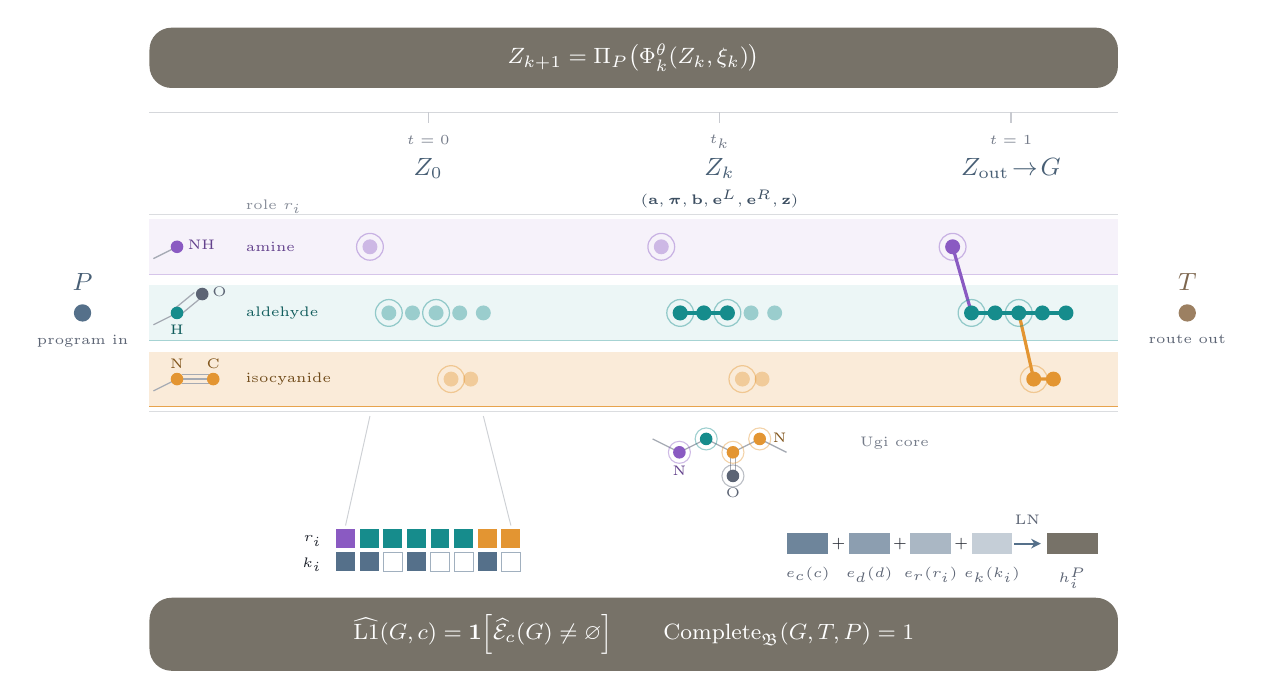
\begin{tikzpicture}[
  font=\scriptsize,
  plate/.style={rounded corners=8pt, fill=navybar, fill opacity=0.79, text opacity=1, text=white, inner xsep=10pt, inner ysep=6pt,
    minimum width=12.30cm, align=center, font=\footnotesize},
  statelab/.style={text=peri!85!black, font=\small},
  lead/.style={-{Stealth[length=3pt,width=3pt]}, draw=peri!75, line width=0.6pt},
]
\definecolor{roleamine}{HTML}{8A5AC2}
\definecolor{roleald}{HTML}{168C8C}
\definecolor{roleiso}{HTML}{E39532}
\definecolor{ground}{HTML}{F4F1E9}
\definecolor{groundcore}{HTML}{D9C9A6}
\colorlet{navybar}{groundcore!38!black}
\definecolor{peri}{HTML}{55708A}
\definecolor{cyanacc}{HTML}{9C8062}
\definecolor{ink}{HTML}{22262F}
\definecolor{inkmuted}{HTML}{5C6474}

\def\sxa{4.54}     % the three state columns, 3.70 apart
\def\cx{8.24}
\def\sxc{11.94}
% Include precursor motifs and role labels in the left margin of each band. The equation
% plates and the complete role/state field share a centre; natural bounds preserve the
% program and route endpoints without adding an asymmetric outer margin.
\def\bandl{1.00}
\def\bandr{13.30}
\def\platecx{7.15}
\def\labx{2.10}    % label column. Set by the tightest pair in the block: "aldehyde" against
                   % the leftmost X_1 atom halo, and "amine" against its own, both ~0.32cm.
\def\inx{0.15}     % P, far enough left that "program in" clears the panel edge
\def\outx{14.18}   % T, mirrored. Not \px/\tx: those are loop variables further down.
\def\ya{0.05}      % trajectory band
\def\yaxis{2.60}   % sampling-time axis, above the molecules
\def\ypanel{-3.15} % coordinate panel
\def\bandh{0.35}   % band half-height. Holds the two-line stratum label; an atom halo is 0.17 of
                   % that, so both clear the band edge. At the original 0.155 the halos
                   % overflowed their own stratum and bled into the neighbouring ones.

%% ================================================================ ground
% A vignette rather than a panel: warm at the centre, fading to the page at the edges, so the
% figure sits on a field with no border to read as an arbitrary rectangle. The large corner
% radius plus the fade gives a lozenge rather than a box.
% Deliberately not an hourglass. In the transition-path figures this shape comes from, the waist
% is the transition state between two basins and the shape is the claim. Here the vertical axis
% is the role coordinate, so a waist would assert that roles merge as sampling proceeds, which
% is false: \Pi_P pins them at every step. The shape stays neutral and the strata carry meaning.
% A two-stop radial is palest exactly where the plates sit, which is what made them read as
% slabs dropped onto white. This is a three-stop field instead: the warm core holds flat out to
% about three quarters of the radius, so it carries past both plates, and only the outer quarter
% fades. The shape is drawn well outside the content so the fade runs off past everything rather
% than stopping at it.
% A vignette, sized a little larger than the drawing so the fade carries past both plates
% instead of stopping level with them.
%% ================================================================ role strata
% The vertical direction is the role coordinate: one stratum per precursor role, and every atom is
% drawn inside its own stratum. This is what makes the background a coordinate system rather than a
% backdrop, and it is only legible because the sites are laid out by role instead of by chemical
% geometry.
% Three strata, not four. This axis is the role coordinate r_i, and r_i ranges over exactly the
% three Ugi-3CR precursor roles: ROLE_NAMES in forge/potency/annotations.py has three entries, and
% forge/model/ugi_joint_sparse_flow.py sizes role_embedding to len(ROLE_NAMES) -- the +1 slot is
% NULL_ROLE_INDEX for the flat ablation arm, not a fourth role. The slate band that used to sit
% here was assembly_introduced from the atlas origin palette, which is an atom origin recovered by
% atom-mapped forward replay after generation, not a coordinate P assigns before sampling. On this
% axis it asserted a fourth precursor role in a three-component reaction.
% Equal-weight bands. The role colours differ widely in intrinsic luminance -- the orange is far
% lighter than the others -- so one shared opacity made isocyanide read as the faintest stratum,
% which asserts an importance ordering the roles do not have. The per-band fill opacity, rule
% opacity and label mix were solved so every band sits the same L* below the ground and every label
% sits at the same L*. Hue separates the roles; value deliberately does not.
% Solved against groundcore, the vignette's centre value, which is what sits under the middle of
% the block. The vignette fades outward, so the equalisation is exact at the centre and drifts
% toward the block's two ends. That drift is close to common-mode -- all three bands span the same
% x range, so they fade together and stay equal to each other -- which is why the vignette can be
% this deep at all. The label mixes are no longer free: a darker band pulls its label toward it, so
% they are solved for one shared L* that is the darkest at which every label still clears 4.5:1
% against its own band. Re-solve all six numbers if groundcore changes again.
% The first column is the stratum offset in mm inside a state scope, which is exactly what
% \forgesites uses to place atoms. Bands and atoms therefore read from one set of numbers.
\foreach \sy/\col/\bandop/\ruleop/\labmix/\lb in {%
       8.4/roleamine/0.079/0.35/72/{amine}/{$\mathrm{N}\text{--}\mathrm{H}$},
       0.0/roleald/0.084/0.38/65/{aldehyde}/{$\mathrm{CH}{=}\mathrm{O}$},
      -8.4/roleiso/0.186/0.84/49/{isocyanide}/{$\mathrm{N}{\equiv}\mathrm{C}$}} {
  \pgfmathsetmacro\yc{\ya+\sy/10}
  \pgfmathsetmacro\ytop{\yc+\bandh}
  \pgfmathsetmacro\ybot{\yc-\bandh}
  \fill[\col, opacity=\bandop] (\bandl,\ybot) rectangle (\bandr,\ytop);
  \draw[\col, opacity=\ruleop, line width=0.4pt] (\bandl,\ybot) -- (\bandr,\ybot);
  \node[font=\tiny, text=\col!\labmix!black, anchor=west] at (\labx,\yc) {\lb};
}
\pgfmathsetmacro\blocktop{\ya+0.84+\bandh+0.06}
\pgfmathsetmacro\blockbot{\ya-0.84-\bandh-0.06}
\pgfmathsetmacro\rolehdr{\blocktop+0.10}
\draw[draw=inkmuted!22, line width=0.35pt] (\bandl,\blocktop) -- (\bandr,\blocktop);
\draw[draw=inkmuted!22, line width=0.35pt] (\bandl,\blockbot) -- (\bandr,\blockbot);
\node[font=\tiny, text=inkmuted!75, anchor=west] at (\labx,\rolehdr) {role $r_i$};

%% ================================================================ what each role contributes
% Read off the reactant side of the same SMARTS:
%   [NX3;H2,H1:1] . [CX3H1:2]=[OX1] . [C;-1,+0;X1:3]#[N;+1,+0;X2:4]
% The open bond means "continues into the precursor", not a substitution count: the amine is
% H2 or H1, so its nitrogen may carry one substituent or two and this commits to neither. The
% aldehyde's oxygen is grey because it is unmapped and does not survive into the product.
\tikzset{frag/.style={line width=0.45pt, draw=inkmuted!55}, lbl/.style={font=\tiny, inner sep=0.6pt}}
\begin{scope}[shift={(1.05,\ya+0.84)}]
  \draw[frag] (0mm,-1.5mm) -- (3.0mm,0mm);
  \fill[roleamine] (3.0mm,0mm) circle (0.8mm);
  \node[lbl, text=roleamine!72!black, anchor=west] at (4.1mm,0.2mm) {NH};
\end{scope}
\begin{scope}[shift={(1.05,\ya)}]
  \draw[frag] (0mm,-1.5mm) -- (3.0mm,0mm);
  \draw[frag] (2.65mm,0.5mm) -- (5.2mm,2.6mm);
  \draw[frag] (3.35mm,-0.3mm) -- (5.9mm,1.8mm);
  \fill[roleald] (3.0mm,0mm) circle (0.8mm);
  \fill[inkmuted] (6.2mm,2.4mm) circle (0.8mm);
  \node[lbl, text=inkmuted, anchor=west] at (7.2mm,2.7mm) {O};
  \node[lbl, text=roleald!65!black, anchor=north] at (3.0mm,-1.3mm) {H};
\end{scope}
\begin{scope}[shift={(1.05,\ya-0.84)}]
  \draw[frag] (0mm,-1.5mm) -- (3.0mm,0mm);
  \foreach \dy in {-0.55,0,0.55} \draw[frag] (3.6mm,\dy mm) -- (7.0mm,\dy mm);
  \fill[roleiso] (3.0mm,0mm) circle (0.8mm);
  \fill[roleiso] (7.6mm,0mm) circle (0.8mm);
  \node[lbl, text=roleiso!57!black, anchor=south] at (3.0mm,1.0mm) {N};
  \node[lbl, text=roleiso!57!black, anchor=south] at (7.6mm,1.0mm) {C};
\end{scope}


%% ================================================================ endpoints
\fill[peri] (\inx,\ya) circle (1.1mm);
\node[font=\small, text=peri!85!black, anchor=south] at (\inx,\ya+0.16) {$P$};
\node[font=\tiny, text=inkmuted, anchor=north] at (\inx,\ya-0.16) {program in};
\fill[cyanacc] (\outx,\ya) circle (1.1mm);
\node[font=\small, text=cyanacc!80!black, anchor=south] at (\outx,\ya+0.16) {$T$};
\node[font=\tiny, text=inkmuted, anchor=north] at (\outx,\ya-0.16) {route out};

%% ================================================================ the three states
% One shared position layout across all three: the reaction-program coordinates are per-position and
% are given by P before sampling starts, so every position keeps its role colour and its core halo
% throughout. Opacity, not colour, carries what the flow actually determines.
\newcommand{\forgesites}[1]{%
  % x is position along the chain, y is the role stratum, so a site's height IS its role coordinate
  \foreach \px/\py/\col/\core in {%
      -7.4/8.4/roleamine/1,
      -5.0/0.0/roleald/1, -2.0/0.0/roleald/0, 1.0/0.0/roleald/1,
       4.0/0.0/roleald/0,  7.0/0.0/roleald/0,
       2.9/-8.4/roleiso/1,  5.4/-8.4/roleiso/0} {
    \ifnum\core=1 \draw[\col, line width=0.45pt, opacity=0.42] (\px mm,\py mm) circle (1.7mm); \fi
    \ifnum#1=1 \fill[\col] (\px mm,\py mm) circle (0.95mm);
    \else \fill[\col, opacity=0.38] (\px mm,\py mm) circle (0.95mm); \fi
  }%
}

\begin{scope}[shift={(\sxa,\ya)}] \forgesites{0} \end{scope}

\begin{scope}[shift={(\cx,\ya)}]
  \draw[roleald, line width=1.15pt] (-5mm,0mm) -- (-2mm,0mm) -- (1mm,0mm);
  \forgesites{0}
  \foreach \px in {-5.0, -2.0, 1.0} \fill[roleald] (\px mm,0mm) circle (0.95mm);
\end{scope}

\begin{scope}[shift={(\sxc,\ya)}]
  \draw[roleald, line width=1.15pt] (-5mm,0mm) -- (7mm,0mm);
  \draw[roleiso, line width=1.15pt] (1mm,0mm) -- (2.9mm,-8.4mm) -- (5.4mm,-8.4mm);
  \draw[roleamine, line width=1.15pt] (-5mm,0mm) -- (-7.4mm,8.4mm);
  \forgesites{1}
\end{scope}

%% ================================================================ sampling-time axis
\draw[draw=inkmuted!26, line width=0.4pt] (\bandl,\yaxis) -- (\bandr,\yaxis);
\foreach \tx/\tl/\sl in {\sxa/{$t=0$}/{$Z_0$}, \cx/{$t_k$}/{$Z_k$}, \sxc/{$t=1$}/{$Z_{\rm out}\!\to\!G$}} {
  \draw[draw=inkmuted!34, line width=0.5pt] (\tx,\yaxis) -- (\tx,\yaxis-0.14);
  \node[font=\tiny, text=inkmuted!85, anchor=north] at (\tx,\yaxis-0.17) {\tl};
  \node[statelab, anchor=north] at (\tx,\yaxis-0.47) {\sl};
}
\node[font=\tiny, text=peri!70!black, anchor=north] at (\cx,\yaxis-0.86)
  {$(\mathbf{a},\boldsymbol{\pi},\mathbf{b},\mathbf{e}^{L},\mathbf{e}^{R},\mathbf{z})$};

%% ================================================================ coordinate panel, centred
% Left half: one column per graph position, in the same order and colours as the sites above, with
% the outermost pair bracketed to their atoms. Right half: the same coordinates entering the
% per-position embedding. Together they are what "reaction-program coordinates" means.
%% ================================================================ the Ugi core
% The product side of the atom-mapped SMARTS, [N:1][CH1:2][C+0:3](=O)[NH1+0:4]. Each atom carries
% the colour of the role that supplies it, so it keys to the three reactant fragments beside the
% strata above. The carbonyl oxygen is grey because it is template_introduced_0 and comes from no
% precursor. Halos mark core membership, the convention the states use for k_i.
\begin{scope}[shift={(7.73,-1.72)}]
  \draw[frag] (-3.4mm,1.7mm) -- (0mm,0mm) -- (3.4mm,1.7mm) -- (6.8mm,0mm)
              -- (10.2mm,1.7mm) -- (13.6mm,0mm);
  \draw[frag] (6.45mm,0mm) -- (6.45mm,-3.0mm);
  \draw[frag] (7.15mm,0mm) -- (7.15mm,-3.0mm);
  \foreach \ax/\ay/\col in {0/0/roleamine, 3.4/1.7/roleald, 6.8/0/roleiso,
                            10.2/1.7/roleiso, 6.8/-3.0/inkmuted} {
    \draw[\col, line width=0.4pt, opacity=0.42] (\ax mm,\ay mm) circle (1.4mm);
    \fill[\col] (\ax mm,\ay mm) circle (0.8mm);
  }
  \node[lbl, text=roleamine!72!black, anchor=north] at (0mm,-1.5mm) {N};
  \node[lbl, text=roleiso!57!black, anchor=west] at (11.6mm,1.9mm) {N};
  \node[lbl, text=inkmuted, anchor=north] at (6.8mm,-4.2mm) {O};
\end{scope}
\node[font=\tiny, text=inkmuted!85, anchor=west] at (9.90,-1.60) {Ugi core};

\begin{scope}[shift={(3.37,\ypanel)}]
  \node[font=\tiny, text=ink, anchor=east] at (-0.6mm,3.05mm) {$r_i$};
  \node[font=\tiny, text=ink, anchor=east] at (-0.6mm,0.05mm) {$k_i$};
  \foreach \i/\col/\core in {0/roleamine/1, 1/roleald/1, 2/roleald/0, 3/roleald/1,
                             4/roleald/0, 5/roleald/0, 6/roleiso/1, 7/roleiso/0} {
    \pgfmathsetmacro\x{\i*3.0}
    \fill[\col] (\x mm,2.2mm) rectangle (\x mm+2.4mm,4.6mm);
    \ifnum\core=1
      \fill[peri] (\x mm,-0.8mm) rectangle (\x mm+2.4mm,1.6mm);
    \else
      \draw[peri!55, line width=0.4pt] (\x mm,-0.8mm) rectangle (\x mm+2.4mm,1.6mm);
    \fi
  }
\end{scope}
\foreach \ax/\i in {-7.4/0, 7.0/7} {
  \pgfmathsetmacro\axcm{\sxa+\ax/10}
  \pgfmathsetmacro\colx{3.37+\i*0.30+0.12}
  \draw[draw=inkmuted!30, line width=0.35pt] (\axcm,-1.26) -- (\colx,\ypanel+0.50);
}

\begin{scope}[shift={(9.10,\ypanel)}]
  \foreach \i/\lb/\op in {0/{$e_c(c)$}/0.85, 1/{$e_d(d)$}/0.68, 2/{$e_r(r_i)$}/0.50, 3/{$e_k(k_i)$}/0.34} {
    \pgfmathsetmacro\x{\i*7.8}
    \fill[peri, opacity=\op] (\x mm,1.4mm) rectangle (\x mm+5.2mm,4.0mm);
    \node[font=\tiny, text=inkmuted, anchor=north] at (\x mm+2.6mm,0.9mm) {\lb};
    \ifnum\i<3 \node[font=\tiny, text=ink] at (\x mm+6.5mm,2.7mm) {$+$}; \fi
  }
  \draw[-{Stealth[length=3.5pt,width=3.5pt]}, draw=peri, line width=0.8pt] (28.8mm,2.7mm) -- (32.2mm,2.7mm);
  \node[font=\tiny, text=inkmuted, anchor=south] at (30.5mm,3.9mm) {LN};
  \fill[navybar, fill opacity=0.79] (33.0mm,1.4mm) rectangle (39.4mm,4.0mm);
  \node[font=\tiny, text=inkmuted, anchor=north] at (36.2mm,0.9mm) {$h_i^{P}$};
\end{scope}

%% ================================================================ equation plates, centred
\node[plate, anchor=south] at (\platecx,2.90)
  {$Z_{k+1}=\Pi_P\!\left(\Phi_k^\theta(Z_k,\xi_k)\right)$};
\node[plate, anchor=north] at (\platecx,-3.56)
  {$\widehat{\mathrm{L1}}(G,c)=\mathbf{1}\!\left[\widehat{\mathcal{E}}_c(G)\neq\varnothing\right]
    \qquad \mathrm{Complete}_{\mathfrak B}(G,T,P)=1$};

\end{tikzpicture}%
}
\caption{\textbf{FORGE generation and route assessment.}
A reaction program fixes assembly roles and core coordinates without selecting precursor identities.
FORGE generates the whole graph, verifies exact assembly replay, and recursively traces its implied
precursors to evidence-qualified materials or an explicit abstention. Colours mark precursor origin;
grey denotes the Ugi template-introduced oxygen. Replay and route closure are computational checks,
not experimental synthesis evidence.}
\label{fig:forge-overview}
\end{figure*}

\subsection{Conditioning on reaction programs}
\label{sec:program-conditioning}
We sample an admissible complete program $P$ from a training-fold program prior and generate $G$ under
the resulting program,
\begin{equation}
    p_\theta(G,P\mid c)=p_{\mathrm{prog}}(P\mid c)\,p_\theta(G\mid P).
\end{equation}
At graph position $i$, the program embedding is
\begin{equation}
    h_i^P=\operatorname{LN}\!\left(
        e_c(c)+e_d(d)+e_r(r_i)+e_k(k_i)
        +\sum_{u=1}^{4}e_{M,u}(M_{r_i,u})
    \right).
\end{equation}
Here, $e_c,e_d,e_r,e_k$ and $e_{M,u}$ are learned embeddings in a shared hidden space, and
$\operatorname{LN}$ denotes layer normalization. The embedding encodes precursor role, reaction-core
status and role-local morphology. The morphology fields determine active positions and fixed or
variable masks. Sampling from the prior specifies these constraints; generation assigns the atom,
bond and topology states within each role. Appendix~\ref{app:program-encoding} specifies the morphology counts and adapter coordinates.

\subsection{Graph representation and discrete flow}
\label{sec:graph-flow}
FORGE generates a categorical tree-plus-closure state. Given a graph $G$ and its selected exact
atom-mapped annotation $\alpha$, the deterministic encoder assigns
\begin{equation}
    X_\star:=\operatorname{Enc}_P(G,\alpha)
    =\left(\mathbf a,\boldsymbol\pi,\mathbf b,
    \mathbf e^L,\mathbf e^R,\mathbf z\right),
\end{equation}
where $\mathbf a$ contains atom states, $\boldsymbol\pi$ parent pointers, $\mathbf b$ tree-bond
states, and $(\mathbf e^L,\mathbf e^R,\mathbf z)$ closure endpoints and bond states.
The padded raw state space $\overline{\mathfrak X}_{N,K_{\rm cl}}$ is finite. Its well-formed subset
$\mathfrak X_{N,K_{\rm cl}}$ enforces a connected tree and at most $K_{\rm cl}$ distinct closure
edges. The structural decoder $\operatorname{Dec}$ maps this subset onto
$\mathfrak G_{N,K_{\rm cl}}$ and maps malformed states to $\bot_{\rm dec}$
(Theorem~\ref{thm:bounded-representation}). Thus every graph within the declared bounded support
has a representation. The production sampler additionally restricts parent candidates and child counts. The representation
result does not imply compatibility with every program or positive probability under a trained model.

For a given $P$, let $\mathcal I(P)$ index the categorical coordinates, each with finite alphabet
$\mathcal X_i(P)$. Pointer alphabets contain only positions permitted by the layout.
The adapter partitions coordinates into fixed positions $\mathcal F(P)$ with values $x_{P,i}$ and
variable positions $\mathcal V(P)$. The set $\Omega_P$ contains raw states within the allowed alphabets that satisfy the fixed
values. It can contain malformed or chemically invalid states. The source law $q_0^P$ fixes
$\mathcal F(P)$ and uses independent, full-support marginals $q_{0,i}^P$ on variable alphabets.
For a clean endpoint $x_1\in\Omega_P$, the conditional corruption law is
\begin{equation}
    q_{t\mid1}^P(x\mid x_1)
    =\mathbf 1[x_{\mathcal F(P)}=x_{P,\mathcal F(P)}]
    \prod_{i\in\mathcal V(P)}
    \left[(1-t)q_{0,i}^P(x_i)+t\mathbf 1\{x_i=x_{1,i}\}\right],
    \quad 0\leq t\leq1.
    \label{eq:conditional-path}
\end{equation}
Each coordinate interpolates between its source and clean value. Their conditional joint law is a
product, so it generally differs from a linear mixture of the joint source and endpoint laws.

The clean-coordinate predictor $d_{\theta,i}(a\mid x,t,P)$ assigns a probability to each
$a\in\mathcal X_i(P)$. A continuous-time Markov chain (CTMC) uses these predictions to average
conditional one-coordinate rates,
\begin{equation}
 R_{t,i}^\theta(u,v\mid x,P)
 =\sum_{a\in\mathcal X_i(P)}d_{\theta,i}(a\mid x,t,P)
 R^*_{t,i}(u,v\mid a,P),\qquad u\neq v,\quad t<1.
 \label{eq:posterior-rate}
\end{equation}
The conditional rate $R^*_{t,i}$ realizes the corresponding factor in
Equation~\ref{eq:conditional-path}; Appendix~\ref{app:flow-proof} defines it and proves the path
identity. The joint generator permits one coordinate to change at an infinitesimal time.
Coordinate posterior marginals therefore suffice to specify its rates, even when endpoint
coordinates are statistically dependent.

\subsection{Program-conditioned Transformer and training}
\label{sec:model-training}

FORGE applies this discrete flow to $X_\star$ and conditions endpoint prediction on $P$. A chemistry
adapter converts the reaction program into masks over atom, pointer and bond coordinates. Program-fixed
coordinates remain constant while the flow generates all remaining states. A graph Transformer
predicts the clean atom, bond, pointer and closure states from $(X_t,t,P)$. Each layer uses
self-attention with relation biases for parent, child and closure edges, then cross-attends to
tokens encoding program identity, depth, precursor role and reaction-core position. Repeating this
cross-attention in every layer makes program information available during both local updates and
coordination between precursor-derived regions. Softly program-routed residual adapters add
family-specific parameters to the shared whole-graph backbone. We supervised role and core annotations
using qualified atom-mapped traces and excluded records with multiple unresolved source traces
from semantic training.

Training records follow a source-balanced distribution $\mu_{\rm bal}$ over annotated triples
$(G,\alpha,P)$, with equal total mass across the three source reaction chemistries. This does not
assign equal mass to every morphology-specific program $P$. The reported final model combines
masked coordinate cross-entropy, role-balanced chemistry, role and core supervision, and repeat
and topology consistency terms. We combined the three chemistry-task gradients using projecting
conflicting gradients (PCGrad) \citep{yu2020gradient}. Appendix~\ref{app:training} specifies the
loss reductions, auxiliary terms and time distribution used for the reported three-family model.

To isolate the statistical property of coordinate denoising, define the reference population loss
\begin{equation}
 \mathcal L_{\rm ref}(\theta)
 =\mathbb E_{\substack{(G,\alpha,P)\sim\mu_{\rm bal},\ t\sim\mathcal U(0,1)\\
 X_t\sim q_{t\mid1}^P(\cdot\mid X_\star)}}
 \left[\sum_{i\in\mathcal V(P)}w_i(P)
 \bigl[-\log d_{\theta,i}(X_{\star,i}\mid X_t,t,P)\bigr]\right],
 \qquad w_i(P)>0.
 \label{eq:primary-loss}
\end{equation}
The weights depend only on the program; they can normalize coordinate counts without depending
on the unknown clean category. This reference loss supports the population analysis. It is not
the complete production training objective.

The reference objective has an ideal population interpretation. For a program with positive training
mass, let $q_1^P$ be the law of $\operatorname{Enc}_P(G,\alpha)$ under $\mu_{\rm bal}(\cdot\mid P)$,
and let $\mu_G^P$ be the corresponding graph law.
\begin{theorem}[Ideal conditional generation]
\label{thm:ideal-terminal-law}
Fix such a program $P$, with registered chemistry $c$, finite coordinate alphabets and a
full-support source on each variable alphabet. Assume every training endpoint belongs to $\Omega_P$, decodes to its source
graph, and passes molecular validity and verified exact L1. Assume an unrestricted measurable
coordinate predictor attains a population minimum of Equation~\ref{eq:primary-loss}. Starting from $q_0^P$, exactly simulate the local CTMC
of Equation~\ref{eq:posterior-rate} on $0\leq t<1$. Then its marginal law converges to $q_1^P$ as
$t\uparrow1$, and
\begin{equation}
 \operatorname{Dec}_{\#}q_1^P=\mu_G^P,\qquad
 \Pr_{G\sim\mu_G^P}\!\left[\mathrm{Valid}(G)=1,
 \widehat{\mathrm{L1}}(G,c)=1\right]=1.
\end{equation}
Here $\operatorname{Dec}_{\#}$ denotes the distribution obtained by decoding.
\end{theorem}
Appendix~\ref{app:flow-proof} proves this result by recovering the clean-coordinate posteriors and
verifying the CTMC forward equation. The theorem concerns the reference population objective and the
limit of exact continuous-time sampling. It establishes neither generalization beyond $q_1^P$ nor
correctness of finite training, PCGrad, capped Euler updates or constrained terminal readout.

\subsection{Sampling and exact assembly verification}
\label{sec:sampling-verification}
The implemented sampler uses discrete states $Z_k$, distinguishing them from the ideal process
$X_t$. Let $\Pi_P$ restore all program-fixed coordinates. Starting from $Z_0\sim q_0^P$, it applies
\begin{equation}
 Z_{k+1}=\Pi_P\!\left(\Phi_k^\theta(Z_k,\xi_k)\right),
 \qquad k=0,\ldots,L_{\rm samp}-1,
 \label{eq:numerical-sampling}
\end{equation}
where $\Phi_k^\theta$ is a capped independent-coordinate Euler update and $\xi_k$ contains its
random draws. Fixed coordinates have zero update rate and remain constant after every projection
(Proposition~\ref{prop:fixed-invariance}). This property constrains the state coordinates;
chemical consistency requires a separate check.

After the final step, the model predicts clean coordinates again at $t=1$. A constrained terminal
readout $H_P^\theta$ selects a state $Z_{\rm out}=H_P^\theta(Z_{L_{\rm samp}})$ or returns a typed
failure. The production readout uses constrained argmax, including the qualified Ugi core-saturation
rules. Structural decoding produces $G$ or a failure; molecular sanitization determines whether the
decoded graph passes the validity check.
Appendix~\ref{app:sampling} specifies these operations and their distinction from ideal CTMC sampling.

For each valid graph, Equation~\ref{eq:main-exact-traces} recovers and verifies the implied
precursors. This establishes consistency with the registered final assembly without restricting
the generator to stored precursors. Molecular validation, candidate decomposition, exact replay
and root ambiguity are recorded separately. The primary yield divides verified exact-L1 attempts by
all generation attempts, including failures.

\subsection{Recursive route assessment}
\label{sec:route-assessment}

For precursors that are not directly available, a bounded program constructor searches for preparation
routes and checks terminal supplier evidence,
\begin{equation}
    Y=\mathsf{Assess}_{\mathfrak B}(G,P,\mathbf C_T,\tau_T)
    \in\mathfrak D\cup\mathfrak F_{\mathfrak B},
\end{equation}
where $\mathfrak D$ is the dossier space, $\mathfrak F_{\mathfrak B}$ is the finite set of typed
outcomes under the frozen route contract $\mathfrak B$, and
$(\mathbf C_T,\tau_T)$ is the sole verifier-returned exact root trace. Ambiguous roots cause an
abstention. A dossier is route-complete only when $G$
passes molecular and exact-assembly verification, each upstream reaction is admitted and verified,
and every required precursor traces to an available starting material. Otherwise the constructor
returns an explicit unresolved or search-censored outcome.

Generation and route assessment remain separate. The reaction program $P$ conditions the distribution
of $G$, whereas $\mathsf{Assess}_{\mathfrak B}$ evaluates the completed graph without modifying it.
Appendix~\ref{app:forge} specifies graph serialization, model training, numerical sampling and
evidence admission, with the complete inference procedure in Algorithm~\ref{alg:forge-inference}.
Appendix~\ref{app:theory} states the assumptions and proofs of the formal results.

\section{Results}
\label{sec:results}

\subsection{Evaluation protocol and matched budgets}

We evaluated FORGE on Ugi, repeated aza-Michael addition and repeated reductive amination using three
matched arms: shared conditioning, shared training without program information and shared training
with cyclically incorrect reaction labels. All arms used the same architecture, optimization budget,
attempt count and prespecified final checkpoint. We evaluated three independent training seeds.
Verified exact-L1 yield is the fraction of generation attempts that passed molecular validation,
program-aware decomposition and exact forward replay. We excluded component-disjoint held-out products from
training and checkpoint selection. Training seeds were the independent units for across-run
comparisons. Appendix~\ref{app:results} contains the full protocol and seed-level results.

Equal attempt budgets account for generation failures. For a fixed model and program, let $p$ be the
probability that one attempt passes molecular validation and verified exact-L1 assembly. Under
independent sampling, the accepted count $A_B$ among $B$ attempts satisfies
\begin{equation}
    A_B\sim\operatorname{Binomial}(B,p),\qquad
    \mathbb E[A_B]=Bp.
\end{equation}
Post-hoc filtering selects accepted outputs but does not change the proposal's $p$. We therefore included every generation attempt in the denominator,
including invalid and unverifiable outputs, and reported coverage separately from replay precision.
The binomial law describes sampling variation for a fixed model. We summarized retraining variation
using the three independent seed-level results.
Proposition~\ref{prop:posthoc-budget} gives the corresponding accepted-count and sampling-cost results.

\subsection{Shared generation achieved exact assembly across three programs}
We first tested whether one conditional flow could learn all three reactions while preserving Ugi
performance. Across
\ForgeProseAttemptsPerProgram{} held-out attempts per program and seed, FORGE achieved verified
exact-L1 yields of \ForgeTableOneConditionedUgiYield\% for Ugi,
\ForgeTableOneConditionedBLYield\% for repeated aza-Michael addition and
\ForgeTableOneConditionedLXYield\% for repeated reductive amination
(Table~\ref{tab:iclr-shared-programs}). Every verifier-returned trace passed exact forward replay in
every program and seed, as required by construction. Reductive amination showed greater between-seed
variation and higher decomposition ambiguity, indicating less consistent learning in this lower-data
setting.

FORGE produced no fixed-coordinate violations or support overflows across
\ForgeProseConditionedTotalAttempts{} held-out attempts. These runs established exact assembly across
all three programs, with the highest yield for Ugi.

\begin{table}[H]
\caption{\textbf{Exact assembly under three ionizable-lipid reaction programs.}
Exact-L1 yields are mean $\pm$ sample standard deviation across three seeds. The final column reports
decomposition coverage and the forward-replay verifier invariant. Per-seed values:
Appendix~\ref{app:results}.}
\label{tab:iclr-shared-programs}
\centering
\small
\setlength{\tabcolsep}{4.6pt}
\begin{tabular}{@{}lcccc@{}}
\toprule
Program & FORGE conditioned & Shared null & Cyclic program &
\shortstack{Decomp. coverage /\\ replay invariant (\%)} \\
\midrule
Ugi & $96.4\pm2.1$ & $34.8\pm7.1$ & $93.8\pm4.2$ & 99.9/100.0 \\
Aza-Michael & $72.2\pm1.6$ & $19.2\pm4.1$ & $71.5\pm2.2$ & 100.0/100.0 \\
Reductive amination & $52.3\pm3.4$ & $37.0\pm2.2$ & $50.7\pm4.9$ & 86.6/100.0 \\
%
\end{tabular}
\end{table}

\subsection{Program conditioning improved exact-assembly yield}
To isolate the effect of reaction information during generation, we compared the conditioned
model with the shared-null and cyclic arms under the same attempt budget and post-hoc verifier.
Shared generation without program information yielded \ForgeTableOneNullUgiYield\%,
\ForgeTableOneNullBLYield\% and \ForgeTableOneNullLXYield\% exact L1 for Ugi, aza-Michael addition
and reductive amination, respectively (Table~\ref{tab:iclr-shared-programs}). For Ugi, conditioning
increased yield by \ForgeTableOneNullUgiDifferencePP{} percentage points (three-seed range
\ForgeTableOneNullUgiRangeLowPP{} to \ForgeTableOneNullUgiRangeHighPP{} points).

Assigning the wrong reaction identity reduced exact-L1 yield to
\ForgeTableOneCyclicUgiYield\%, \ForgeTableOneCyclicBLYield\% and
\ForgeTableOneCyclicLXYield\% across the three programs. The cyclic control retained precursor roles, reaction-core
coordinates and program depth, isolating the contribution of the reaction-identity label within a
structured program. The larger conditioned-versus-null differences supported a benefit from program
information during generation. The small conditioned-versus-cyclic differences did not establish
a strong independent contribution from the identity label.

\subsection{Decoder and architecture effects differed across programs}
Exact assembly depends on both the learned distribution and terminal decoding. In a seed-0 diagnostic
with trained weights held fixed, enforcing the qualified Ugi core's hydrogen states increased exact-L1 yield relative to
valence-only topology decoding, while molecular validity was nearly unchanged
(Appendix~\ref{app:ablation-results}). The core-saturation constraint changed the generated graph, and
we applied the same exact-replay verifier to both decoders. Molecular validity alone therefore did
not account for the improvement in reaction consistency. Changing the initial corruption
distribution from program-role marginals to global marginals also reduced yield. These fixed-model
diagnostics complement the independently retrained comparisons in Table~\ref{tab:iclr-shared-programs}.

A separate three-seed mechanism study compared whole-graph denoising with a parameter-matched
component-factorized model (FACT), which generates precursor roles independently
(Appendix~\ref{app:ablation-results}). Its full-Transformer control was trained independently of
the production model. Mean exact-L1 products per 1,000 attempts were
\ForgeProseMechanismFullUgi{} versus \ForgeProseMechanismFactMatchedUgi{} for Ugi and
\ForgeProseMechanismFullBL{} versus \ForgeProseMechanismFactMatchedBL{} for aza-Michael addition.
The direction reversed for reductive amination:
\ForgeProseMechanismFullLX{} versus \ForgeProseMechanismFactMatchedLX{}. Increasing FACT capacity
did not reverse these mean orderings. Joint denoising improved exact assembly in two programs. The negative
conditional-dependence diagnostic left the mechanism of this advantage unresolved.

Individual modules likewise had mixed effects. Removing layerwise program cross-attention reduced
Ugi and reductive-amination yield but increased aza-Michael yield; removing gradient-conflict control
slightly improved all three means. The ablations did not support a uniform benefit
from every module across the tested reaction programs.

\subsection{Generated precursors extended beyond the training catalogues}
We next asked whether FORGE could preserve exact assembly while generating precursor constitutions
absent from training. Under the common Ugi benchmark, the finite-inventory methods produced
\ForgeProseCommonSelectorExactPerThousand{} verified exact-L1 products per 1,000 attempts but zero
component-novel products by construction. FORGE produced
\ForgeProseCommonForgeExactPerThousand{} verified products and
\ForgeProseCommonForgeDistinctPerThousand{} distinct component-novel products per 1,000 attempts
(Table~\ref{tab:ugi-common-benchmark}).

\begin{table}[htbp]
\caption{\textbf{Exact Ugi assembly with precursor constitutions absent from
method-visible training.} Values are mean $\pm$ sample standard deviation per 1,000 attempts across
three seeds under a common component-disjoint protocol and verifier. Component-novel is
verifier-relative and does not establish strong product-level catalogue escape. Whole-molecule
baselines are assessed post hoc. $\dagger$, structural zero; N/E, not estimable.}
\label{tab:ugi-common-benchmark}
\centering
\scriptsize
\setlength{\tabcolsep}{2.2pt}
% Column 1 is fixed so the numeric columns, not the model names, decide the table's natural
% width. The generated rows separate the three baseline groups with a rule and no heading.
% 3.3cm is the widest model name ("Learned inventory selector", 92.4pt) plus a little; the
% \resizebox is a guard, since the header arrows push the natural width just past the block.
\resizebox{\textwidth}{!}{%
\begin{tabular}{@{}>{\raggedright\arraybackslash}p{3.3cm}cccccc@{}}
\toprule
Models & \shortstack{Valid / 1,000\\$\uparrow$} &
\shortstack{Verified L1 / 1,000\\$\uparrow$} &
\shortstack{Distinct L1 / 1,000\\$\uparrow$} &
\shortstack{Comp.-novel / 1,000\\$\uparrow$} &
\shortstack{Held-comp. / 1,000\\$\uparrow$} & Diversity \\
\midrule
RGFN & $0.0\pm0.0$ & $0.0\pm0.0$ & $0.0\pm0.0$ & $0.0\pm0.0^{\dagger}$ & $0.0\pm0.0$ & N/E \\
\midrule
DeFoG unconditional & $346.5\pm42.3$ & $280.6\pm26.6$ & $280.6\pm26.6$ & $280.6\pm26.6$ & $15.5\pm2.4$ & $0.727\pm0.014$ \\
GenMol/SAFE & $627.5\pm6.2$ & $0.0\pm0.0$ & $0.0\pm0.0$ & $0.0\pm0.0$ & $0.0\pm0.0$ & $0.873\pm0.009$ \\
\midrule
Learned inventory selector & $1000.0\pm0.0$ & $1000.0\pm0.0$ & $849.5\pm13.7$ & $0.0\pm0.0^{\dagger}$ & $0.0\pm0.0$ & $0.717\pm0.001$ \\
Finite catalogue oracle & $1000.0\pm0.0$ & $1000.0\pm0.0$ & $837.6\pm8.2$ & $0.0\pm0.0^{\dagger}$ & $0.0\pm0.0$ & $0.719\pm0.000$ \\
Shared-null + post-hoc & $194.7\pm15.6$ & $114.4\pm10.9$ & $108.5\pm9.7$ & $108.5\pm9.7$ & $0.4\pm0.2$ & $0.754\pm0.014$ \\
FACT-matched & $60.8\pm20.2$ & $52.0\pm15.6$ & $50.8\pm14.4$ & $50.8\pm14.4$ & $0.0\pm0.0$ & $0.667\pm0.009$ \\
FACT-generous & $500.7\pm213.8$ & $296.7\pm186.0$ & $288.3\pm175.3$ & $288.3\pm175.3$ & $0.1\pm0.2$ & $0.774\pm0.007$ \\
\midrule
\cellcolor{forgerow}FORGE &\cellcolor{forgerow} $965.0\pm21.9$ &\cellcolor{forgerow} $963.9\pm21.4$ &\cellcolor{forgerow} $862.6\pm19.2$ &\cellcolor{forgerow} $862.6\pm19.2$ &\cellcolor{forgerow} $1.4\pm1.7$ &\cellcolor{forgerow} $0.643\pm0.022$ \\
%
\end{tabular}
}
\end{table}

Against the fixed training catalogues, component-novel verified exact-L1 yields reached
\ForgeProseCatalogueForgeUgiComponentNovelPerThousand{},
\ForgeProseCatalogueForgeBLComponentNovelPerThousand{} and
\ForgeProseCatalogueForgeLXComponentNovelPerThousand{} products per 1,000 attempts across Ugi,
aza-Michael addition and reductive amination. The corresponding finite catalogues had zero
component-novel yield by construction (Appendix~\ref{app:novelty-results}). Representative Ugi
products are shown in Figure~\ref{fig:forge-generated-samples}.

Among the external baselines, DeFoG produced \ForgeProseCommonDefogExactPerThousand{} verified
products and recovered held components more often than FORGE
(\ForgeProseCommonDefogHeldPerThousand{} versus \ForgeProseCommonForgeHeldPerThousand{} per 1,000
attempts). GenMol/SAFE produced no exact Ugi-L1 product, and RGFN emitted no admissible output. FORGE therefore combined reaction consistency with verifier-relative component novelty,
although DeFoG recovered the reserved components more often. Product-level catalogue escape
remained unmeasured.

Component novelty also did not establish recovery of the held-out lipid distribution. The
method-blind realism analysis measured both precision and coverage in fingerprint and descriptor
spaces, together with a source-study-grouped classifier two-sample test
(Appendix~\ref{app:novelty-results}). No evaluated method reproduced the full held-out observed-lipid
distribution. The measured expansion was limited to reaction-consistent molecular identities.
Neither diversity nor distance from training established agreement with observed lipid structures
or biological utility.

\begin{figure}[htbp]
\caption{\textbf{Exact Ugi products with recovered precursors absent from training.}
Each row contains a deterministic seed-0 product with a unique verified exact-L1 decomposition and a
verifier-recovered precursor absent from training. Columns show the generated lipid and its recovered
precursors. These are
structural examples, not evidence of activity or experimental synthesis success.}
\label{fig:forge-generated-samples}
\centering
% Vector drawings use the unchanged frozen sample identities; see the chemical_drawings receipt.
\newlength{\samplerowheight}\setlength{\samplerowheight}{4.2cm}
\newlength{\sampleproductwidth}\setlength{\sampleproductwidth}{0.465\textwidth}
\newlength{\sampleprecursorwidth}\setlength{\sampleprecursorwidth}{0.49\textwidth}
\newcommand{\iclrsamplerow}[1]{%
\begin{minipage}[c][\samplerowheight][c]{\sampleproductwidth}\centering
\includegraphics[width=\linewidth]{figures/chemical_drawings/sample_#1_product.pdf}
\end{minipage}
&
\begin{minipage}[c][\samplerowheight][c]{\sampleprecursorwidth}\centering
\includegraphics[width=\linewidth]{figures/chemical_drawings/sample_#1_precursors.pdf}
\end{minipage}}
\setlength{\tabcolsep}{0pt}
\resizebox{\textwidth}{!}{%
\begin{tabular}{@{}c@{\hspace{2.6mm}}!{\color{atlasrule}\vrule width 0.5pt}@{\hspace{2.6mm}}c@{}}
\toprule
\atlashead{\sampleproductwidth}{Generated lipid}
& \atlashead{\sampleprecursorwidth}{Exact L1 building blocks}\\
\midrule
\addlinespace[1.2mm]
\iclrsamplerow{01}\\
\addlinespace[2.2mm]
\iclrsamplerow{02}\\
\addlinespace[0.6mm]
\bottomrule
\end{tabular}
}
\end{figure}

\subsection{Precursor evidence limited complete route construction}
To assess whether the verified assemblies had complete computational synthesis dossiers, we checked
precursor preparation and terminal-material evidence in addition to exact L1 replay.
Only \ForgeCommonRouteEvidenceCompleteComponents{} of \ForgeCommonRouteUnionComponents{} components
in the frozen evidence union closed under the exact-source library. FORGE therefore produced
\ForgeCommonRouteForgeExactPerThousand{} verified exact-L1 products per 1,000 attempts but
\ForgeCommonRouteForgeCompletePerThousand{} complete dossiers. In a route-blind sample of
\ForgeRouteCandidates{} products, \ForgeRouteCompleteProducts{} closed,
\ForgeRouteUnresolvedProducts{} were unresolved and \ForgeRouteCensoredProducts{} were
search-censored (Appendix~\ref{app:route-results}). These outcomes measured completion under the
frozen evidence policy. The syntheses of unresolved products remain unknown.



\subsection{Exploratory in vivo reporter imaging of three synthesized designs}
\label{sec:in-vivo}

To examine reporter expression from experimentally prepared designs, we synthesized three lipids
from the shared three-family model, designated FORGE-1, FORGE-2 and FORGE-3, and formulated them
with firefly luciferase (FLuc) mRNA. At the 4-hour time point, the reported region-of-interest (ROI)
signals were $5.997\times10^5$, $2.036\times10^6$ and $2.881\times10^6$, respectively, compared
with $2.195\times10^5$ for the MC3 formulation (Figure~\ref{fig:in-vivo}). All three recorded FORGE
values exceeded the recorded MC3 value. These observations support reporter expression in this
exploratory experiment. The record contains one reported value per formulation; it does not support
estimating between-animal variability or a statistical comparison. The synthesis and formulation
information is given in Appendix~\ref{app:in-vivo-methods}.
% Author confirmation pending: biological n, animal/site allocation, ROI units and background
% correction, administration route, and candidate/checkpoint identifiers. The author confirmed
% all three structures originated from the historical three-family model. Do not infer n=1
% per formulation from the single reported value, or count the three designs as replicates.

\begin{figure}[htbp]
\centering
\begin{minipage}[t]{0.56\textwidth}
\vspace{0pt}
\small\textbf{a}\quad Synthesized FORGE lipids\\[7pt]
\footnotesize FORGE-1\\[3pt]
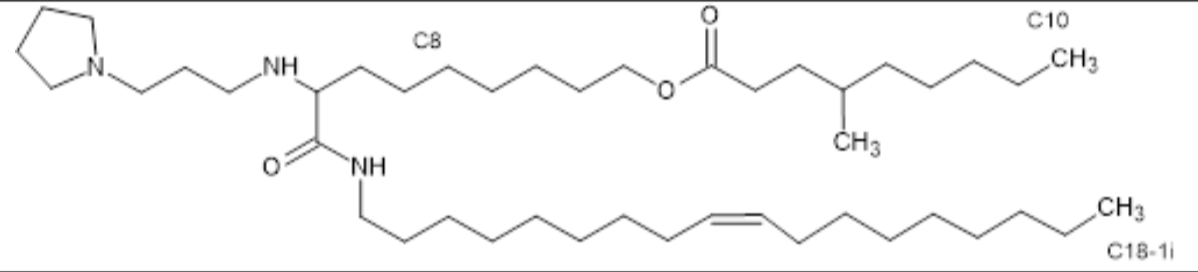
\includegraphics[width=\linewidth]{experimental/in_vivo/forge_1_structure_supplied.png}\\[9pt]
\footnotesize FORGE-2\\[3pt]
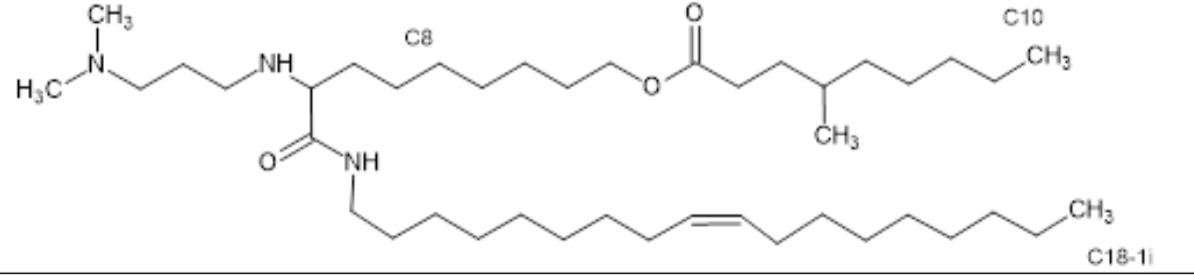
\includegraphics[width=\linewidth]{experimental/in_vivo/forge_2_structure_supplied.png}\\[9pt]
\footnotesize FORGE-3\\[3pt]
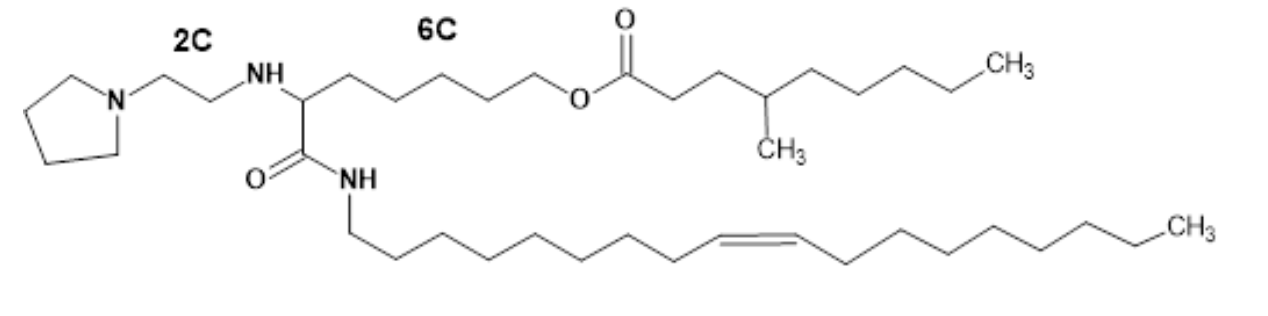
\includegraphics[width=\linewidth]{experimental/in_vivo/forge_3_structure_supplied.png}
\end{minipage}\hfill
\begin{minipage}[t]{0.39\textwidth}
\vspace{0pt}
\small\textbf{b}\quad Mouse bioluminescence image\\[7pt]
\includegraphics[width=\linewidth]{experimental/in_vivo/mouse_imaging_supplied.png}
\end{minipage}

\par\vspace{14pt}
\begin{minipage}[t]{\textwidth}
\small\textbf{c}\quad Reported 4-hour signals\par\vspace{7pt}
\centering
\pgfplotstableread[col sep=comma]{experimental/in_vivo/reported_roi_values.csv}\forgeinvivotable
\pgfplotstablegetelem{3}{reported_roi_signal}\of{\forgeinvivotable}
\begingroup
\pgfkeys{/pgf/fpu=true}
\pgfmathparse{\pgfplotsretval/1000000}
\pgfmathfloattofixed{\pgfmathresult}
\global\let\forgeMCThreeSignal\pgfmathresult
\endgroup
\begin{tikzpicture}
\begin{axis}[
 width=0.92\linewidth,height=5.5cm,
 scale only axis=false,
 xmin=-0.6,xmax=3.6,ymin=0,ymax=3.2,
 xtick={0,1,2,3},ytick={0,1,2,3},
 xticklabels={FORGE-1,FORGE-2,FORGE-3,MC3},
 ylabel={Reported ROI signal ($\times10^6$)},
 tick label style={font=\footnotesize},label style={font=\footnotesize},
 axis lines*=left,axis line style={black!65},tick style={black!65},
 ymajorgrids=true,grid style={black!10},
 nodes near coords={\pgfmathprintnumber[fixed,precision=4]{\pgfplotspointmeta}},
 every node near coord/.append style={font=\footnotesize,anchor=south},
 legend style={at={(0.98,0.98)},anchor=north east,draw=none,fill=none,font=\footnotesize},
 legend cell align=left,
 clip=false]
\addplot[ybar,bar width=26pt,bar shift=0pt,draw=none,fill=blue!50!gray,
 restrict x to domain=-0.5:2.5,filter discard warning=false,forget plot]
 table[col sep=comma,x expr=\coordindex,y expr=\thisrow{reported_roi_signal}/1000000]
 {experimental/in_vivo/reported_roi_values.csv};
\addplot[ybar,bar width=26pt,bar shift=0pt,draw=none,fill=black!60,
 restrict x to domain=2.5:3.5,filter discard warning=false,forget plot]
 table[col sep=comma,x expr=\coordindex,y expr=\thisrow{reported_roi_signal}/1000000]
 {experimental/in_vivo/reported_roi_values.csv};
\addplot[red!65!gray,dashed,line width=0.8pt,no marks,nodes near coords={}]
 coordinates {(-0.6,\forgeMCThreeSignal) (3.6,\forgeMCThreeSignal)};
\addlegendentry{MC3 level}
\end{axis}
\end{tikzpicture}
\end{minipage}
\caption{\textbf{Structures and exploratory in vivo FLuc imaging measurements.}
\textbf{a}, Structures of FORGE-1, FORGE-2 and FORGE-3 from the shared three-family model.
Structure drawings are reproduced as supplied; stereochemical identity was not established by the
constitutional generator.
\textbf{b}, Original mouse imaging record, with all four ROI boundaries and numerical labels
preserved. ROI 1--4 display the values assigned to FORGE-1, FORGE-2, FORGE-3 and MC3 in panel c.
\textbf{c}, Reported ROI values at the 4-hour time point, without aggregation or error estimates.
The dashed red line marks the MC3 signal.
Bars denote reported values, not a declared number of independent animals. The signal-unit and
replicate information needed for a quantitative delivery comparison remains unresolved; the plotted
values are descriptive.}
\label{fig:in-vivo}
\end{figure}
\FloatBarrier

\section{Discussion}

FORGE conditions whole-molecule generation on known assembly chemistry with precursor identities
left open. Across the three specified programs, conditioning increased verified exact-L1 yield
relative to matched generation followed by post-hoc verification. Generated products also contained
verifier-recovered precursors absent from the training catalogues. The combination of complete
molecular generation and exact assembly replay permits exploration beyond the supplied precursor
identities without requiring a finite component inventory in the generative state.

The evidence supports component-level expansion under the registered chemistry. Complete
catalogue-product reachability was not computed, so the results do not establish strong
product-level catalogue escape. Held-component recovery was weak
(\ForgeProseCommonForgeHeldPerThousand{} products per 1,000 attempts), and no evaluated method
reproduced the full held-out lipid distribution. Joint denoising and individual architectural
modules also had reaction-dependent effects. Higher exact-assembly yield therefore did not imply
uniform gains in generalization, structural realism or every reaction program.

Route assessment further bounded the demonstrated capability. Exact final assembly does not
establish precursor availability, and the bounded evidence library left the final-model products
without complete dossiers. Neither synthesis guidance nor the bounded potency diagnostic improved
the matched outcome (Appendix~\ref{app:results}). These computational comparisons cover three
programs within bounded graph support. Evidence was strongest for Ugi; extending qualified precursor
evidence and testing additional supported programs would address the limits of route completion
and chemical coverage.

The exploratory mouse measurements extend the study to reporter expression from three synthesized
designs. Their recorded signals exceeded the recorded MC3 signal, but the available measurements
do not establish reproducibility across animals, a population-level advantage over MC3, tissue
selectivity, tolerability or therapeutic efficacy. This experiment also does not retrospectively
complete the frozen computational synthesis dossiers. Candidate-specific synthesis records and the
L2/L3 evidence required by that assessor are distinct from a reporter-imaging measurement.

\subsection*{AI use statement}
Generative AI tools assisted with conceptual and methodological development, software implementation
and debugging, experimental design and diagnostic analysis, interpretation of computational results,
literature search and summarization, and drafting and editing the manuscript. The authors are
responsible for the final code, reported results, citations and conclusions, including material
produced with AI assistance.

\subsection*{Ethics statement}
This work evaluates ionizable-lipid generation computationally and includes exploratory mouse
bioluminescence measurements with three synthesized FORGE lipids. Animal procedures were approved
by Children's Hospital of Philadelphia. Molecular design systems can be misused. Chemical validity, exact assembly verification, synthesis-route evidence and predicted
properties do not establish safety or biological efficacy. The reported mouse measurements do not
establish tolerability, tissue selectivity or therapeutic efficacy. Generated compounds without
experimental measurements remain computational candidates requiring further evaluation before use.

\subsection*{Reproducibility statement}
The Methods and Appendix specify the molecular representation, conditional discrete flow, numerical
sampler, exact assembly verification, route assessment, benchmark protocols and evaluation metrics.
Appendix~\ref{app:repro} summarizes randomization, historical implementation provenance and the
access limitations of the standalone manuscript archive. Seed-level results appear in
Appendix~\ref{app:results}; assumptions and proofs appear in Appendix~\ref{app:theory}.

\bibliographystyle{iclr2027_conference}
\bibliography{forge,references}

\clearpage
\appendix

\section{Method and implementation details}
\label{app:forge}

This appendix specifies program and graph encoding, model training, sampling, verification and
route assessment. Algorithm~\ref{alg:forge-inference} combines the inference steps.

\subsection{Reaction-program encoding}
\label{app:program-encoding}

The program tuple in Equation~\ref{eq:reaction-program} uses the ordered atom-position set
$\mathcal I_{\rm atom}(P)=\{1,\ldots,n(P)\}$. The arrays $\mathbf r$ and $\mathbf k$ assign
precursor roles and core positions to these atoms. This atom-position index differs from
$\mathcal I(P)$, which indexes all six families of categorical coordinates.

Morphology is computed from the selected atom-mapped trace and its sparse serialization.
For role $r$, let $V_r^{\rm ext}$ contain its exterior atoms, excluding reaction-core atoms, and
let $o_r(v)$ count the same-role exterior children of $v$ in the serialized tree. The four fields are
\begin{equation}
 M_r=(n_r,j_r,\gamma_r,a_r),\qquad
 n_r=|V_r^{\rm ext}|,\qquad
 j_r=\sum_{v\in V_r^{\rm ext}}\max\{o_r(v)-1,0\}.
\end{equation}
Here $\gamma_r$ counts closure edges with both endpoints in $V_r^{\rm ext}$, and $a_r$ counts
same-role bonds between exterior and core atoms. When the serialized tree restricts to a spanning
forest of the exterior subgraph, $\gamma_r$ equals that subgraph's cycle rank. The junction budget
is a tree-branching count; it does not count degree contributed by closure bonds. Consequently these
fields depend on the selected annotation and serialization, not on the unannotated graph alone.
Fixed-coordinate equality alone does not establish agreement with every morphology field.
Positions without precursor origin use the designated absent morphology state. Integer morphology
values are encoded with an offset of one, reserving zero for that absent state.

The training-fold prior and program embeddings are defined in Section~\ref{sec:program-conditioning}.
A chemistry-specific adapter determines the precursor roles, reaction core, reverse decomposition
and forward transform associated with $c$. Its sampling layout determines active positions and
fixed or variable coordinates; the embeddings condition neural prediction on the remaining
program fields.

\subsection{Graph serialization and source annotations}
\label{app:graph-encoding}

A spanning-tree representation with at most three residual closure edges preserves the full
194-atom support without an $O(N_{\max}^2)$ edge state. The discrete flow generates the atom, bond
and topology states in this representation.
Let $\alpha=(\mathbf C,\tau,\mathbf r,\mathbf k)$ contain the selected exact precursor tuple,
registered assembly trace, atom-wise precursor-role assignment and reaction-core annotation. The deterministic
program-aware encoder
\begin{equation}
    \operatorname{Enc}_P:
    \{(G,\alpha):G\in\mathfrak G_{N_{\max},K_{\rm cl}}
      \text{ and }\alpha\text{ is admitted for }P\}
    \longrightarrow \mathfrak X_{N_{\max},K_{\rm cl}}
\end{equation}
constructs the categorical graph state
\begin{equation}
    X_\star:=\operatorname{Enc}_P(G,\alpha)=
    \left(
        \mathbf{a},
        \boldsymbol{\pi},
        \mathbf{b},
        \mathbf{e}^{L},
        \mathbf{e}^{R},
        \mathbf{z}
    \right)
\end{equation}
where $\mathbf{a}$ contains atom states, $\boldsymbol{\pi}$
parent pointers, $\mathbf{b}$ spanning-tree bond states, $\mathbf{e}^{L}$ and $\mathbf{e}^{R}$
closure-endpoint pointers, and $\mathbf{z}$ closure-bond states.

The encoder first partitions the atoms into connected precursor-origin components under $\alpha$.
It selects as root the reaction-core atom with the smallest tie-broken canonical RDKit rank, and
orders the origin-component graph by breadth-first traversal from that root component, breaking
ties by role index, component canonical ranks and original atom index. Within each component it uses
a deterministic depth-first preorder from the selected attachment atom, with neighbors ordered by
the same canonical ranks. The traversed bonds define the spanning tree. Every residual bond is
represented once as an ordered endpoint pair with its bond label, and residual triples are sorted
lexicographically. Role, core, fixed-coordinate and morphology arrays follow the
same atom order. We excluded training records with more than one qualified exact source trace
from semantic training and collapsed duplicate descriptions of an admitted trace to its canonical
record. Thus
$\operatorname{Dec}(\operatorname{Enc}_P(G,\alpha))\cong G$ for every admitted record.

The raw padded categorical product space $\overline{\mathfrak X}_{N_{\max},K_{\rm cl}}$ also
contains malformed states. Its well-formed subset $\mathfrak X_{N_{\max},K_{\rm cl}}$ enforces an
active node prefix, earlier-parent pointers, distinct valid closure endpoints, no duplicate edges,
and null values in unused closure slots. The total decoder, including its failure value, is typed as
\begin{equation}
    \operatorname{Dec}:\overline{\mathfrak X}_{N_{\max},K_{\rm cl}}
    \longrightarrow
    \mathfrak G_{N_{\max},K_{\rm cl}}\cup\{\bot_{\rm dec}\}.
\end{equation}
For this study, $N_{\max}=194$ and $K_{\rm cl}=3$.
These bounds specify architectural support. Reaction consistency, nonzero probability under a
trained model and synthesis-program completeness require separate conditions.

The structural decoder specifies graph reconstruction from an already chosen state.
The production terminal readout additionally chooses that state from neural predictions
(Appendix~\ref{app:sampling}). These are separate operations.

The chemistry adapter marks any atom, pointer, or bond states fixed by $P$.
FORGE holds these states constant while corrupting the remaining states along the linear probability
path and predicting their clean values from $(X_t,t,P)$. Let $\Omega_P$ be the subset of the raw state
space satisfying the allowed coordinate alphabets and fixed values, and define the admissible program set
\begin{equation}
    \mathcal P_{\rm adm}
    =\left\{P:\mathfrak X_{N_{\max},K_{\rm cl}}\cap\Omega_P\neq\varnothing\right\}.
\end{equation}
The morphology prior is normalized only on $\mathcal P_{\rm adm}$. Each chemistry adapter is required
to satisfy the program-compatible encoding property: every admitted annotated record obeys
$\operatorname{Enc}_P(G,\alpha)\in\Omega_P$. During corpus construction, we checked this property and exact constitutional decode round trip
for every record before split assignment. Records failing either check were excluded. The checks
covered all cached training, calibration and held-out records; they do not establish the property
for unregistered chemistry.

\subsection{Transformer architecture and training objectives}
\label{app:training}

The denoiser is a graph Transformer over the complete sparse state. Each layer applies graph
self-attention with relation biases for parent, child and closure edges, then cross-attends to memory
tokens representing program identity, program depth, precursor role and reaction-core position.
Cross-attention is repeated in every layer so that reaction semantics can influence both local state
updates and long-range coordination among precursor-derived regions. Three softly program-routed
residual adapters add family-specific parameters to the shared whole-graph backbone.

The reported final three-family model used a stratified minibatch with 21 records per chemistry
and source-weighted sampling within each stratum. Two such microbatches formed an optimizer update.
Training times were $t=\min\{0.98,\max\{0.02,U\}\}$ for $U\sim\mathcal U(0,1)$, giving point
masses of $0.02$ at both endpoints and unit density on $(0.02,0.98)$. Thus training did not cover
all times required by the ideal reference objective in Equation~\ref{eq:primary-loss}.

For chemistry $c$ and state family
$q\in\mathscr J=\{\mathbf a,\boldsymbol\pi,\mathbf b,\mathbf e^L,\mathbf e^R,\mathbf z\}$,
let $\mathcal S_{c,q}$ be the selected variable coordinates across that chemistry's minibatch.
With coordinate loss $\ell_i=-\log d_{\theta,i}(X_{\star,i}\mid X_t,t,P)$, the pooled reduction is
\begin{equation}
 L_{c,q}^{\rm pool}=\frac{\sum_{i\in\mathcal S_{c,q}}\ell_i}{\max\{1,|\mathcal S_{c,q}|\}}.
\end{equation}
Coordinates here include their example index. Chemistry states (atoms, parent bonds and closure
bonds) additionally use equal mass over roles present in the selected coordinates. If
$\mathcal S_{c,q,r}$ contains coordinates assigned to role $r$ and
$\mathcal R_{c,q}=\{r:|\mathcal S_{c,q,r}|>0\}$, this reduction is
\begin{equation}
 L_{c,q}^{\rm role}=\frac{1}{|\mathcal R_{c,q}|}
 \sum_{r\in\mathcal R_{c,q}}\frac{\sum_{i\in\mathcal S_{c,q,r}}\ell_i}{|\mathcal S_{c,q,r}|},
 \label{eq:role-balanced-loss}
\end{equation}
with zero loss if no role is present. Atom and parent-bond groups use their position's role;
closure-bond groups use the role at the clean left endpoint. Pointer losses use the pooled reduction
and mask logits to the permitted layout positions. The flow term $L_{c,\rm flow}$ sums these six
reduced losses, with unit weights.

For each chemistry, the recorded task loss was
\begin{equation}
\begin{aligned}
 L_c={}&L_{c,\rm flow}
 +0.25L_{c,\rm role}+0.25L_{c,\rm core}+0.25L_{c,\rm repeat}\\
 &+L_{c,\rm child}+0.5L_{c,\rm junction}+L_{c,\rm chem\mid top}.
\end{aligned}
\label{eq:production-task-loss}
\end{equation}
The role and core terms are cross-entropies averaged equally over present target states.
The repeat term averages squared differences between predicted atom distributions, and separately
parent-bond distributions, at aligned exterior positions in repeated component instances; it sums
the two means. The child term is state-balanced cross-entropy for same-component exterior child
counts in $\{0,1,2,3\}$. The junction term applies smooth-L1 loss to predicted and target
role-local junction totals, each divided by the number of exterior atoms in that role, then averages
over eligible examples within a role and equally across present roles. Predicted junction totals
sum the expected child-count contribution $\max\{o-1,0\}$ across exterior atoms.
The topology-conditioned chemistry term repeats the role-balanced atom and bond losses in a second
forward pass with clean parent and closure endpoints and corrupted atom and bond states.
These definitions describe the reported final arm; the earlier architecture study used its own
recorded ablation settings.

PCGrad combines the task gradients in integer chemistry-state order. For
$g_c=\nabla_\theta L_c$, it initializes $\widetilde g_c=g_c$ and, for each other task $h$ in that
order, applies
\begin{equation}
 \widetilde g_c\leftarrow\widetilde g_c-
 \mathbf1\{\langle\widetilde g_c,g_h\rangle<0\}
 \frac{\langle\widetilde g_c,g_h\rangle}{\max\{\|g_h\|_2^2,10^{-12}\}}\,g_h
\end{equation}
on parameter coordinates available to both tasks. Gradients are not norm-normalized, and the
optimizer receives the arithmetic mean of the projected task gradients. This update is not generally
the gradient of a scalar sum of task losses. No population optimality claim is made for the full
procedure. In particular, target-dependent group reductions and the restricted training-time range
require analysis beyond Proposition~\ref{prop:masked-bayes}.

We tested layerwise cross-attention, each auxiliary loss, routed adapters and gradient-conflict
control through separate interventions (Appendix~\ref{app:ablation-results}).

\subsection{Numerical sampling and terminal decoding}
\label{app:sampling}

The finite sampler evaluates the denoiser at $t_k=k/L_{\rm samp}$, for
$k=0,\ldots,L_{\rm samp}-1$, and uses $\Delta t=1/L_{\rm samp}$.
Conditional on $Z_k=x$, it draws one clean category
$A_{k,i}\sim d_{\theta,i}(\cdot\mid x,t_k,P)$ independently for each variable coordinate.
Write $s_{t,i}^P(u\mid a)=(1-t)q_{0,i}^P(u)+t\mathbf1\{u=a\}$ for its conditional path factor,
$\dot s_i^P(u\mid a)=\mathbf1\{u=a\}-q_{0,i}^P(u)$ for the derivative, and
$[z]_+=\max\{z,0\}$. The code uses the conditional off-diagonal rate
\begin{equation}
 R_{t,i}^{*,\varepsilon}(u,v\mid a,P)
 =\frac{[\dot s_i^P(v\mid a)-\dot s_i^P(u\mid a)]_+}
 {|\mathcal X_i(P)|\max\{s_{t,i}^P(u\mid a),\varepsilon\}},
 \quad u\neq v,\qquad \varepsilon=10^{-8}.
 \label{eq:clamped-rate}
\end{equation}
Full source support is required only on the allowed coordinate alphabet, including the masked
candidate set for a pointer. Thus that alphabet is the support for every $t_k<1$.
The denominator clamp in Equation~\ref{eq:clamped-rate} is a numerical safeguard absent from the
ideal rate in Appendix~\ref{app:flow-proof}.

For the sampled endpoint $a=A_{k,i}$, let
$h_{k,i}=\Delta t\sum_{v\neq x_i}R_{t_k,i}^{*,\varepsilon}(x_i,v\mid a,P)$ and set
$\kappa_{k,i}=\min\{1,0.999/h_{k,i}\}$ when $h_{k,i}>0$, with $\kappa_{k,i}=1$ otherwise.
The implemented coordinate kernel is
\begin{equation}
 \widehat K_{k,i}(v\mid x,a)=
 \begin{cases}
 \kappa_{k,i}\Delta t\,R_{t_k,i}^{*,\varepsilon}(x_i,v\mid a,P),&v\neq x_i,\\
 1-\kappa_{k,i}h_{k,i},&v=x_i.
 \end{cases}
 \label{eq:capped-kernel}
\end{equation}
Its off-diagonal masses sum to at most $0.999$; the diagonal is the remaining mass. Consequently
all entries are nonnegative and each row sums to one. Coordinates are drawn independently from
these kernels, followed by the projection $\Pi_P$.

Without the clamp or cap, and when every conditional Euler row is nonnegative, averaging over
$A_{k,i}$ gives the Euler kernel built from Equation~\ref{eq:posterior-rate} exactly. One sampled
endpoint per coordinate therefore does not by itself bias that uncapped one-step law. The nonlinear
cap generally changes the averaged kernel. Independent coordinate updates also permit simultaneous
finite-step changes, so their product is a numerical approximation to the local CTMC, not its exact
transition kernel. No discretization error bound is asserted near the terminal singularity.

After all steps, the model evaluates $(Z_{L_{\rm samp}},1,P)$ once more. The production terminal
readout $H_P^\theta$ selects coordinate values using constrained argmax, restores fixed states and
returns either a raw state or a typed terminal failure, denoted collectively by $\bot_{\rm term}$.
For Ugi it enforces one hydrogen on the aldehyde-derived $\alpha$ carbon and one on the
isocyanide-derived amide nitrogen. The selected state is then reconstructed and checked for
connectedness, valence and sanitization. A readout failure retains its detailed reason in the ledger;
for graph-law notation we extend $\operatorname{Dec}(\bot_{\rm term})=\bot_{\rm dec}$.
If $q_{\theta,\rm out}^P$ is the law after terminal readout, including failure, then
\begin{equation}
 p_\theta(\cdot\mid P)=\operatorname{Dec}_{\#}q_{\theta,\rm out}^P,
 \qquad
 p_\theta(G\mid P)=\sum_{z:\operatorname{Dec}(z)=G}q_{\theta,\rm out}^P(z).
 \label{eq:generated-law}
\end{equation}
This law retains structural failures and chemically invalid graphs before the validity and L1
filters; it is not conditioned on acceptance.
The ideal theorem does not include the learned $t=1$ readout, which is unconstrained by a loss
integrated over $t\in(0,1)$. We compared core-saturation and valence-only readouts under the same
trained weights and verifier, then separately compared program-role and global source marginals
(Appendix~\ref{app:ablation-results}).

\subsection{Exact assembly verification}
\label{app:verification}

For the chemistry $c$ specified by $P$, FORGE decomposes each valid graph into role-assigned
precursors and applies the registered forward transform. Exact replay checks assembly existence
under $c$; it does not test full agreement with the sampled conditioning layout.

\begin{definition}[Exact assembly and recovered witnesses]
\label{def:exact-assembly}
For the registered forward operator $\mathcal F_c$ on precursor inputs $\mathfrak C_c$, define
\begin{equation}
 \mathcal E_c^\star(G)=\{\mathbf C\in\mathfrak C_c:G\in\mathcal F_c(\mathbf C)\},\qquad
 \mathrm{L1}^\star(G,c)=\mathbf1\{\mathcal E_c^\star(G)\neq\varnothing\}.
\end{equation}
The bounded reverse procedure returns candidate pairs $(\mathbf C,\tau)$ in $\mathcal D_c(G)$.
Equation~\ref{eq:main-exact-traces} retains the pairs passing exact forward replay, and
\begin{equation}
 \widehat{\mathrm{L1}}(G,c)=\mathbf1\{\widehat{\mathcal E}_c(G)\neq\varnothing\}.
\end{equation}
Both predicates describe assembly existence; molecular validity is checked separately.
\end{definition}
The set $\mathcal E_c^\star(G)$ contains precursor inputs, whereas
$\widehat{\mathcal E}_c(G)$ contains input--trace pairs. Their compatible comparison is
\begin{equation}
 \{\mathbf C:\exists\tau,\ (\mathbf C,\tau)\in\widehat{\mathcal E}_c(G)\}
 \subseteq\mathcal E_c^\star(G),\qquad
 \widehat{\mathrm{L1}}(G,c)\leq\mathrm{L1}^\star(G,c).
\end{equation}
The inclusion follows directly from exact replay. Its converse requires complete reverse search,
which has not been established. Throughout the paper, verified exact-L1 yield counts valid
attempts satisfying the recovered predicate. Candidate traces are compared after the registered
role- and step-aware canonicalization, so duplicate encodings do not create additional witnesses.

Post-hoc filtering changes which completed samples are retained but cannot change the proposal
distribution's exact-L1 acceptance probability.
Under independent sampling, this probability determines the complete distribution of accepted
counts under a fixed attempt budget and the expected cost of obtaining a fixed number of accepted
products (Proposition~\ref{prop:posthoc-budget}).
We distinguish decomposition coverage from forward-replay precision because a candidate disconnection
may fail to reconstruct $G$.
Candidate decomposition coverage is the fraction of valid graphs for which
$\mathcal D_c(G)\neq\varnothing$. For a declared sequence of valid evaluation graphs $G_1,\ldots,G_m$, candidate replay precision is
\begin{equation}
 \mathrm{ReplayPrecision}
 =\frac{\sum_{b=1}^m|\widehat{\mathcal E}_c(G_b)|}
 {\sum_{b=1}^m|\mathcal D_c(G_b)|},
\end{equation}
with N/E when the denominator is zero. Replay of tuples already in
$\widehat{\mathcal E}_c(G)$ has $100\%$ success by construction. This invariant does not estimate
candidate replay precision. We separately define
\begin{equation}
 \mathrm{CandidateAmbig}(G,c)=\mathbf 1\{|\mathcal D_c(G)|>1\},\qquad
 \mathrm{ExactAmbig}(G,c)=\mathbf 1\{|\widehat{\mathcal E}_c(G)|>1\}.
\end{equation}
A distinct exact-L1 product is a deduplicated generated constitution. An unambiguous exact
decomposition satisfies $|\widehat{\mathcal E}_c(G)|=1$. We distinguish product uniqueness from
decomposition uniqueness throughout.

\subsection{Recursive route assessment and dossier admission}
\label{app:route-assessment}

\subsubsection{Assessment interface}

For a valid generated graph $G$ and reaction program $P$ with chemistry $c$, route assessment
returns either a
complete synthesis dossier or a typed abstention.
Let $\mathfrak B$ denote the frozen route contract: depth and query budgets, registered transforms,
evidence-admission rules and a dated supplier snapshot. Let $\mathfrak D$ be the space of candidate
dossiers, each containing a synthesis tree and its reaction and terminal evidence, and let
$\mathfrak F_{\mathfrak B}$ be the disjoint finite set of typed failures.
Generation and assessment are defined by
\begin{equation}
    Y=\mathsf{Assess}_{\mathfrak B}(G,P,\mathbf C_T,\tau_T)
    \in\mathfrak D\cup\mathfrak F_{\mathfrak B}.
\end{equation}
$\mathsf{Assess}_{\mathfrak B}$ is invoked after the verifier returns one admitted root trace
$(\mathbf C_T,\tau_T)\in\widehat{\mathcal E}_c(G)$. It verifies the final assembly, searches for
preparation routes to unavailable precursors and checks terminal supplier evidence. $P$ and the assessor act at different stages: $P$ guides generation, whereas the assessor
constructs a dossier from the completed graph without modifying it.
FORGE accepts $(G,T)$ only when $G$ passes molecular and exact-assembly verification and $T$ traces
every required precursor to an available starting material; otherwise, it abstains.

\subsubsection{Recursive expansion and completion checks}

Completing a synthesis dossier requires evidence for every recovered precursor. Exact L1
verification specifies the precursor structures; availability and preparation routes require
additional evidence. Each precursor must therefore match an available material or have a supported
route from available starting materials.
Let $T$ be a candidate dossier with bipartite synthesis tree $(V_M,V_R,E_T)$ rooted at $G$, where each product molecule
points to its preparation reaction and each reaction points to its required reactants.
The assessor constructs these routes recursively and withholds a complete dossier when any branch
remains unresolved.
A molecule node terminates when a current, dated supplier record lists an exact constitutional match
as available; otherwise, FORGE must expand that node through a supported, forward-verified reaction.
FORGE uses a bounded level-two (L2) planner to propose each expansion.
For each proposal, FORGE records the reaction, reactants, product, and supporting evidence, and
accepts the step only when the forward transform reconstructs the target precursor exactly.
Each accepted reaction adds its reactants as new molecule nodes, and FORGE applies the same
termination-or-expansion rule recursively.
The current assessor admits only an unambiguous verified exact-L1 root. Every dossier therefore
records the sole selected root trace
$(\mathbf C_T,\tau_T)\in\widehat{\mathcal E}_c(G)$; an ambiguous exact set produces a typed
abstention. For each upstream reaction node $r$, let
$\mathrm{Admitted}_{\mathfrak B}(r)=1$ when its reaction and substrate scope satisfy the frozen
evidence policy, and let $\mathrm{Verify}_{\mathfrak B}(r)=1$ when
$\operatorname{target}(r)\in\mathcal F_r(\operatorname{reactants}(r))$.
For each leaf molecule $\ell$, let $\mathrm{Available}_{\mathfrak B}(\ell)=1$ when it satisfies the terminal
supplier-evidence rule.
Let $V_R^{\mathrm{up}}(T)$ denote the upstream preparation-reaction nodes and $L(T)$ the leaf
molecules. $\mathrm{WellFormed}(G,T,P)$ requires that $T$ is a connected, acyclic bipartite tree
rooted at $G$; each internal molecule has exactly one recorded producing reaction; no molecular constitution repeats along an ancestor path; each reaction's
molecule children equal its recorded reactants with their multiplicities; and $T$ has no disconnected, cyclic or
extraneous node. Its distinguished final-assembly record must have product $G$ and precursor
children exactly $\mathbf C_T$ under trace $\tau_T$.
\begin{equation}
\begin{aligned}
    \mathrm{Complete}_{\mathfrak B}(G,T,P)
    ={}&\mathrm{Valid}(G)\,\mathrm{WellFormed}(G,T,P)\\
    &\times\mathbf1\!\left[\widehat{\mathcal E}_c(G)=\{(\mathbf C_T,\tau_T)\}\right]\\
    &\times\prod_{r\in V_R^{\mathrm{up}}(T)}
    \mathrm{Admitted}_{\mathfrak B}(r)\mathrm{Verify}_{\mathfrak B}(r)
    \prod_{\ell\in L(T)}\mathrm{Available}_{\mathfrak B}(\ell).
\end{aligned}
\end{equation}
All factors are binary and empty products equal one. Repeated use of a material is represented by
separate tree occurrences; equality of their constitutions does not merge their nodes.
Under finite search bounds and terminating evidence queries, the assessor terminates and returns a
dossier only when $\mathrm{Complete}_{\mathfrak B}(G,T,P)=1$
(Lemma~\ref{lem:planner-termination} and Invariant~\ref{inv:dossier-soundness}).
An abstention means that FORGE did not complete a dossier under $\mathfrak B$; it does not imply that
no synthesis route exists outside the frozen search space or evidence snapshot.
The guarantee is computational and does not establish experimental synthesis success.

\subsubsection{Recorded evidence and support tiers}

For each accepted pair $(G,T)$, the synthesis dossier contains every molecule and reaction in $T$,
the evidence for each reaction and a dated supplier record for each terminal material.
We classify assembly support relative to the fixed reference space into four tiers:
\textbf{E0 (enumerated):} the generated lipid matches a product that was already constructed
computationally from known components using a supported reaction.
\textbf{E1 (known components):} the generated lipid was not included in the bounded E0 enumeration,
but a supported reaction assembles it entirely from known components.
\textbf{E2 (generated precursor):} a supported reaction assembles the lipid, but at least one
precursor is newly generated and requires a complete L2 route to available starting materials.
\textbf{E3 (new assembly family):} the lipid requires a final assembly reaction outside the
qualified reaction registry.

\subsection{End-to-end inference procedure}
\label{app:inference}

Algorithm~\ref{alg:forge-inference} records every generation attempt, including failures in
molecular validation, exact replay or route completion.

% Ruled caption and procedure; paragraph spacing is internal to the algorithmic list.
\begingroup
\setlength{\parskip}{0pt}
\hrule height 0.8pt\kern 2pt
\refstepcounter{algorithm}
\noindent\textbf{Algorithm~\thealgorithm} FORGE generation and fail-closed synthesis-program construction.
\label{alg:forge-inference}
\par\nobreak\kern 2pt\hrule height 0.4pt\nobreak
\begin{algorithmic}[1]
\Require trained coordinate predictors, chemistry $c$, program prior $p_{\rm prog}(\cdot\mid c)$,
integers $L_{\rm samp}\geq1$ and $B\geq0$, recorded seed $s$, route contract $\mathfrak B$
\Ensure attempt-indexed dossier sequence $\mathcal D_{\rm out}$, exact-L1 ledger $\mathcal L_{\rm out}$,
and typed failure ledger $\mathcal H$
\State initialize the random-number streams from $s$;
$\mathcal D_{\rm out}\gets[\,]$; $\mathcal L_{\rm out}\gets[\,]$; $\mathcal H\gets[\,]$
\For{$b=1,\ldots,B$}
    \State sample and record $P\sim p_{\rm prog}(\cdot\mid c)$
    \State sample $Z_0\sim q_0^P$ and set $Z\gets\Pi_P(Z_0)$
    \For{$k=0,\ldots,L_{\rm samp}-1$}
        \State $t_k\gets k/L_{\rm samp}$; $\Delta t_k\gets1/L_{\rm samp}$
        \State $Z\gets\Pi_P\!\left(\Call{CappedCoordinateEuler}{Z,t_k,\Delta t_k,P}\right)$
    \EndFor
    \State $Z_{\rm out}\gets H_P^\theta(Z)$ \Comment{fresh prediction at $t=1$, constrained readout}
    \If{$Z_{\rm out}$ is a terminal failure}
        \State record $(b,\textsc{TerminalFailure},\text{readout reason})$ in $\mathcal H$; \textbf{continue}
    \EndIf
    \State $G\gets\operatorname{Dec}(Z_{\rm out})$
    \If{$G=\bot_{\rm dec}$ or $\mathrm{Valid}(G)=0$}
        \State record $(b,\textsc{InvalidGraph},\text{decode or validation reason})$ in $\mathcal H$
        \State \textbf{continue}
    \EndIf
    \State $\widehat{\mathcal{E}}_c(G)\gets
    \{(\mathbf C,\tau)\in\mathcal D_c(G):\exists H\in\mathcal F_c(\mathbf C),\ H\cong G\}$
    \If{$\widehat{\mathcal{E}}_c(G)=\varnothing$}
        \State $\mathcal H\gets\mathcal H\mathbin{\|}[(b,\textsc{L1Failure})]$
        \State \textbf{continue}
    \EndIf
    \State $\mathcal L_{\rm out}\gets\mathcal L_{\rm out}\mathbin{\|}
    [(b,G,\widehat{\mathcal E}_c(G))]$
    \If{$|\widehat{\mathcal E}_c(G)|\neq1$}
        \State $\mathcal H\gets\mathcal H\mathbin{\|}[(b,\textsc{AmbiguousL1})]$
        \State \textbf{continue}
    \EndIf
    \State select the sole $(\mathbf C_T,\tau_T)\in\widehat{\mathcal E}_c(G)$
    \State $Y\gets\mathsf{Assess}_{\mathfrak B}(G,P,\mathbf C_T,\tau_T)$
    \If{$Y$ is a dossier $T$ and $\mathrm{Complete}_{\mathfrak B}(G,T,P)=1$}
        \State $\mathcal D_{\rm out}\gets\mathcal D_{\rm out}\mathbin{\|}
        [(b,T)]$
    \ElsIf{$Y\in\mathfrak F_{\mathfrak B}$}
        \State $\mathcal H\gets\mathcal H\mathbin{\|}[(b,Y)]$
    \Else
        \State $\mathcal H\gets\mathcal H\mathbin{\|}[(b,\textsc{IncompleteDossier})]$
    \EndIf
\EndFor
\State \Return $\mathcal D_{\rm out},\mathcal L_{\rm out},\mathcal H$
\end{algorithmic}
\nopagebreak\hrule height 0.8pt
\endgroup

\subsection{Reproducibility and artifact provenance}
\label{app:repro}

The computational results use the historical shared three-family model. Training-seed labels
0, 1 and 2 correspond to random-number seeds 20260825, 20260826 and 20260827, respectively
(Table~\ref{tab:production-seed-counts}). Each comparison retains its declared training split,
attempt budget, checkpoint rule and evaluator. The manuscript provenance records identify the
source artifacts for the reported tables and figures through SHA-256 hashes.

The historical source verification matched the complete seed-0 evaluation-source fingerprint to
a retained code snapshot. No exact match was recovered for the seed-1 and seed-2 evaluation-source
fingerprint among the retained snapshots inspected, and a complete training-source manifest was
not recovered. These limits and the checked per-seed settings are recorded in the accompanying
\nolinkurl{mathematical_review.json}. Current development code does not establish the historical
implementation used for those runs.

The standalone manuscript archive contains the LaTeX source, generated tables, figure assets and
provenance records. It does not bundle the training corpora, model checkpoints, full evaluation
ledgers or a complete historical training-environment and compute manifest. Independent end-to-end
reruns therefore require access to the corresponding historical run artifacts. The supplied
experimental images and ROI values are included; the unresolved experimental details are described
in Section~\ref{sec:in-vivo} and Appendix~\ref{app:in-vivo-methods}.

\clearpage

\section{Evaluation protocol and additional results}
\label{app:results}

The evaluation protocol applies to Section~\ref{sec:results}. Additional analyses quantify
decomposition outcomes, variation across training seeds, component diversity and the bounded guidance
diagnostics. Each comparison includes its seed-level results and metric definitions.

\FloatBarrier
\subsection{Evaluation protocol}
\label{app:evaluation-protocol}

\subsubsection{Data, splits and generation budgets}

We evaluated three assembly programs with different amounts of supervision: Ugi, repeated
aza-Michael addition and repeated reductive amination. The comparisons tested shared generation,
reaction conditioning, recovery of precursors absent from training and completion of synthesis
dossiers. We trained three matched shared-model arms: correct program conditioning, no program
information and cyclically incorrect reaction labels. All arms used the same architecture and
optimization budget. We evaluated the prespecified final checkpoint from three independent training
seeds under equal generation-attempt budgets per program.
Our primary metric is verified exact-L1 yield per generation attempt: the number of generated graphs that
pass molecular validity, program-aware decomposition, and exact forward replay divided by the total
number of sampling attempts.
Secondary metrics separate graph quality (validity and connectedness), reaction recovery (verified
coverage, the replay invariant, abstention, and exact ambiguity), and exploration (distinct-product fraction, whole-product and
component novelty, molecular diversity, and effective component count).
We report exact counts, means across seeds, sample standard deviations, individual seed values, and
the minimum and maximum of the three paired seed contrasts. These are descriptive across-seed
summaries, not confidence intervals. Generated molecules are not treated as independent training
replicates. Conditional binomial variation across a fixed model's
\ForgeProseAttemptsPerProgram{} attempts is distinct from
variation induced by retraining.
Training used only the component-disjoint training folds. We used calibration data for diagnostics
and excluded held-out products from training and checkpoint selection. All three shared arms
assigned equal total sampling mass to each program and preserved the frozen within-program source
weights.
We also checked the prespecified numerical acceptance criteria. With three training seeds, these
checks describe the observed runs and do not establish population-level non-inferiority. Zero program-fixed-coordinate violations are an implementation check required by
Proposition~\ref{prop:fixed-invariance}, not learned behavior.

\subsubsection{Comparators and matched controls}

The null and cyclic controls tested different aspects of conditioning. Null generation followed
by exact post-hoc filtering measured performance without program information. The cyclic arm
isolated the reaction-identity label with the remaining program structure retained. A separate
train-only finite-component assembler received the exact training components, supported forward
chemistry, source-weighted role marginals and the same number of attempts. We evaluated reaction
validity and exploration separately because catalogue assembly has zero input-component novelty
by construction. None of these comparisons called an L2 planner, biological oracle or
candidate-selection procedure.

For Ugi, we evaluated a common external-baseline protocol with one
reaction-space comparator, RGFN, and two generic whole-molecule comparators, unconditional DeFoG
and GenMol/SAFE \citep{koziarski2024rgfn,qin2025defog,lee2025genmol}.
The Synthesis-DAG method of \citet{ou2024deep}, SynFlowNet and SynCoGen were discussed as related methods and were
excluded from the empirical comparison \citep{cretu2025synflownet,rekesh2025syncogen}.
At the version checks used to construct the benchmark, the Synthesis-DAG repository lacked the
paper-specific ionizable-lipid implementation, the SynFlowNet action space did not support the
qualified three-reactant Ugi transform, and the SynCoGen repository lacked a usable code license.
We preserved each method's native reaction operations and included numerical results only from
executions using the common training split, attempt budget, seed set and molecular and exact-L1
evaluator. The comparison excludes published scores from other datasets and unsupported
aza-Michael or reductive-amination runs.
The matched internal suite included unconditioned generation plus post-hoc filtering, an
oracle finite-catalogue assembler, a learned inventory selector, two learned component-factorized
generators, and targeted interventions on the Transformer. Appendix~\ref{app:ablation-results}
reports the three-seed Transformer mechanism and component-factorization study. Each
intervention used the same folds, generation budget and evaluation code as the full Transformer.

\subsubsection{Metrics, molecular identity and uncertainty}

Let $Y_{s,a,b}^{\rm L1}\in\{0,1\}$ indicate verified exact L1 for training seed $s$, arm $a$ and
attempt $b$, and let $B=\ForgeProseAttemptsPerProgram$. We report the exact count
$C_{s,a}^{\rm L1}=\sum_{b=1}^B Y_{s,a,b}^{\rm L1}$ and
\begin{equation}
 \widehat p_{s,a}^{\rm L1}=C_{s,a}^{\rm L1}/B.
\end{equation}
Validity and connected yield replace $Y^{\rm L1}$ with their attempt-level indicators. Verified
decomposition coverage is the number of valid graphs with
$\widehat{\mathcal E}_c(G)\neq\varnothing$ divided by valid graphs; the implementation does not
report candidate-search coverage before replay. Exact ambiguity is the fraction of valid graphs with
$|\widehat{\mathcal E}_c(G)|>1$. Replay of members of $\widehat{\mathcal E}_c(G)$ is an invariant,
whereas candidate replay precision is defined in Appendix~\ref{app:verification}. The evaluated
artifacts do not retain the pre-replay candidate sets, so candidate-search coverage and candidate
replay precision were not estimated.
Explicitly, with attempt outcomes $G_{s,a,b}$ and the convention that a failed decode makes every
graph predicate zero,
\begin{align}
 \widehat p^{\rm valid}_{s,a}
 &=B^{-1}\sum_b\mathbf 1\{\mathrm{Valid}(G_{s,a,b})=1\},\\
 \widehat p^{\rm conn}_{s,a}
 &=B^{-1}\sum_b\mathbf 1\{\mathrm{Valid}(G_{s,a,b})=1,
                              \mathrm{Connected}(G_{s,a,b})=1\},\\
 \mathrm{CandidateCoverage}
 &=\frac{\sum_b\mathbf 1\{\mathrm{Valid}(G_b)=1,
                              \mathcal D_c(G_b)\neq\varnothing\}}
         {\sum_b\mathbf 1\{\mathrm{Valid}(G_b)=1\}},\\
 \mathrm{ExactAmbiguity}
 &=\frac{\sum_b\mathbf 1\{\mathrm{Valid}(G_b)=1,
                              |\widehat{\mathcal E}_c(G_b)|>1\}}
         {\sum_b\mathbf 1\{\mathrm{Valid}(G_b)=1\}}.
\end{align}
Each ratio is N/E when its denominator is zero.

Distinct-product yield counts canonical constitutions once. The reported verifier-recovered
component-novel yield also counts distinct products and requires an unambiguous recovered input
with an out-of-training-catalogue precursor. It does not measure strong catalogue escape
(Definition~\ref{def:catalogue-escape}). Held-component recovery counts qualifying attempts,
including duplicate products, whose unambiguous input contains a designated held constitution.

For one chemistry $c$, suppress seed and arm indices. Let $\mathcal A_{\rm L1}$ contain the attempt indices
with valid graphs and verified exact L1, and let
$\mathcal A_{\rm one}=\{b\in\mathcal A_{\rm L1}:|\widehat{\mathcal E}_c(G_b)|=1\}$.
For $b\in\mathcal A_{\rm one}$, write the sole recovered input as $\mathbf C_b$, with components $C_{b,j}$
and roles $r_{b,j}$. Let $\mathcal C_{{\rm train},r}$ and $\mathcal H_{{\rm held},r}$ be the
training and designated held constitution sets for role $r$, respectively. Define
\begin{align}
 \mathcal A_{\rm novel}&=\{b\in\mathcal A_{\rm one}:\exists j,\ C_{b,j}\notin\mathcal C_{{\rm train},r_{b,j}}\},\\
 \mathcal A_{\rm held}&=\{b\in\mathcal A_{\rm one}:\exists j,\ C_{b,j}\in\mathcal H_{{\rm held},r_{b,j}}\}.
\end{align}
With $\operatorname{can}$ denoting constitutional canonicalization, the yields for $B>0$ are
\begin{align}
 \mathrm{DistinctL1Yield}&=\frac{|\{\operatorname{can}(G_b):b\in\mathcal A_{\rm L1}\}|}{B},\\
 \mathrm{ComponentNovelYield}&=\frac{|\{\operatorname{can}(G_b):b\in\mathcal A_{\rm novel}\}|}{B},\\
 \mathrm{HeldComponentYield}&=\frac{|\mathcal A_{\rm held}|}{B}.
\end{align}
Reported values per 1,000 attempts multiply these ratios by 1,000. Ambiguous decompositions do not
contribute to the component-novel or held-component numerators.

For a fixed role, let $n_i$ be the occurrence count of component identity $i$ among unambiguous
exact-L1 inputs. When $n_{\rm tot}=\sum_i n_i>0$, set $w_i=n_i/n_{\rm tot}$ and compute
\begin{equation}
 N_{\rm eff}=\exp\!\left(-\sum_{i:n_i>0}w_i\log w_i\right).
\end{equation}
This is the exponential of Shannon entropy with natural logarithms. Duplicate products and repeated
component occurrences contribute to the counts; $N_{\rm eff}$ is N/E when $n_{\rm tot}=0$.
Molecular diversity is the mean pairwise
ECFP4 Tanimoto distance among distinct valid canonical product constitutions, so molecular duplicates
are removed for that metric. For distinct products $g_1,\ldots,g_m$,
\begin{equation}
 \mathrm{Diversity}=
 \frac{2}{m(m-1)}\sum_{1\leq i<j\leq m}
 \left[1-\mathrm{Tanimoto}\bigl(\mathrm{ECFP4}(g_i),\mathrm{ECFP4}(g_j)\bigr)\right],
\end{equation}
with N/E for $m<2$. Every other undefined conditional denominator is likewise reported N/E.

Identity is constitutional and stereo-free. Graph and product identity use connected canonical RDKit
SMILES with atom maps and stereochemical tags removed; formal charges and bond orders are retained;
salts or disconnected products are invalid; and no tautomer normalization is applied. Precursor
identity uses the same canonicalization. Precursor-tuple equality is role- and program-step-aware,
with repeated inputs compared in their registered step order. Training atom mappings and recovered assembly traces serve different roles. The former establish
semantic alignment; the latter record precursor assignments and reaction steps. Neither is part
of constitutional identity.

For a paired contrast, $D_s=\widehat p_{s,\rm FORGE}-\widehat p_{s,\rm control}$. We report
$(D_1,D_2,D_3)$, $\overline D$, and $[\min_sD_s,\max_sD_s]$. These summarize the three observed
training seeds and are not 95\% confidence intervals. Conditional on one fixed trained model,
$C_{s,a}^{\rm L1}$ has the finite-attempt binomial variation in
Proposition~\ref{prop:posthoc-budget}; that uncertainty does not substitute for independent
retraining. Unless explicitly named primary, architecture, coordinate, guidance, potency and
catalogue contrasts are exploratory and no multiplicity-adjusted inferential claim is made.

\FloatBarrier
\subsection{Assembly quality and program conditioning}
\label{app:assembly-results}

\subsubsection{Shared generation across three chemistries}

The full shared-model comparison used \ForgeProseAttemptsPerProgram{} held-out generation attempts
per program in each of three independent training seeds (Table~\ref{tab:production-comparison}).
Table~\ref{tab:iclr-shared-programs} summarizes the exact-L1 yields.
Every verifier-returned trace passed forward replay, as required by the verifier invariant. Mean exact-
decomposition ambiguity was \ForgeTableOneBLAmbiguityPercent\% for repeated aza-Michael addition
and \ForgeTableOneLXAmbiguityPercent\% for
repeated reductive amination, and the latter program showed substantial between-seed variation.
Table~\ref{tab:production-comparison} reports molecular validity, connectedness, decomposition
coverage, forward-replay precision, abstention, ambiguity, novelty and diversity separately for
each program.

The final conditioned model recorded zero fixed-coordinate violations and zero support overflows across
\ForgeProseConditionedTotalAttempts{} held-out attempts (three seeds, three programs and
\ForgeProseAttemptsPerProgram{} attempts per program).
Exact-assembly yields differed across reaction families despite preservation of all fixed
coordinates and graph-support bounds.

% The compact shared-program table is in the main paper as Table~\ref{tab:iclr-shared-programs}.

\begin{table*}[htbp]
\caption{\textbf{Matched shared-model production comparison across reaction programs.}
Point estimates report the mean across three independent seeds; the exact-L1 column additionally
reports the sample standard deviation. Paired contrasts are summarized by their three seed values,
mean and observed range. Conditioned-model counts by seed appear in
Table~\ref{tab:production-seed-counts}.
Validity and connectedness use all generation attempts as the denominator.
Decomposition coverage, replay precision, abstention and ambiguity retain their prespecified
conditional denominators. Novelty is conditioned on valid products or unique returned
decompositions, as appropriate. Fraction pairs and exact-L1 yield are percentages; diversity is
mean pairwise ECFP4 distance and $N_{\mathrm{eff}}$ is the effective generated-component count.
Results are never pooled across reaction programs.}
\label{tab:production-comparison}
\centering
\scriptsize
\setlength{\tabcolsep}{3.5pt}
\resizebox{\textwidth}{!}{%
\begin{tabular}{@{}lccccccccc@{}}
\hline
& \multicolumn{3}{c}{Ugi} & \multicolumn{3}{c}{Aza-Michael}
& \multicolumn{3}{c}{Reductive amination} \\
\cmidrule(lr){2-4}\cmidrule(lr){5-7}\cmidrule(lr){8-10}
& FORGE & Shared null & Cyclic & FORGE & Shared null & Cyclic
& FORGE & Shared null & Cyclic \\
\hline
Valid./Conn. & \cellcolor{forgerow} 96.5/96.5 & 35.9/35.9 & 93.9/93.9 & \cellcolor{forgerow} 72.2/72.2 & 27.4/27.4 & 71.5/71.5 & \cellcolor{forgerow} 60.4/60.4 & 41.9/41.9 & 59.1/59.1 \\
Decomp./Replay & \cellcolor{forgerow} 99.9/100.0 & 97.0/100.0 & 99.8/100.0 & \cellcolor{forgerow} 100.0/100.0 & 69.5/100.0 & 100.0/100.0 & \cellcolor{forgerow} 86.6/100.0 & 88.4/100.0 & 85.7/100.0 \\
Abst./Ambig. & \cellcolor{forgerow} 0.1/0.0 & 3.0/0.9 & 0.2/0.0 & \cellcolor{forgerow} 0.0/61.0 & 30.5/29.3 & 0.0/62.3 & \cellcolor{forgerow} 13.4/74.7 & 11.6/76.6 & 14.3/73.8 \\
Exact-L1/attempt & \cellcolor{forgerow} $96.4\pm2.1$ & $34.8\pm7.1$ & $93.8\pm4.2$ & \cellcolor{forgerow} $72.2\pm1.6$ & $19.2\pm4.1$ & $71.5\pm2.2$ & \cellcolor{forgerow} $52.3\pm3.4$ & $37.0\pm2.2$ & $50.7\pm4.9$ \\
Whole/Comp. novelty & \cellcolor{forgerow} 99.5/96.7 & 99.9/99.0 & 99.4/96.9 & \cellcolor{forgerow} 89.8/85.3 & 99.6/99.7 & 90.2/86.3 & \cellcolor{forgerow} 67.4/97.5 & 91.5/99.8 & 66.0/97.0 \\
Diversity/$N_{\mathrm{eff}}$ & \cellcolor{forgerow} 0.643/419.9 & 0.680/439.5 & 0.646/427.9 & \cellcolor{forgerow} 0.593/118.0 & 0.707/413.5 & 0.603/119.4 & \cellcolor{forgerow} 0.776/173.0 & 0.761/193.3 & 0.773/157.8 \\
%
\end{tabular}
}
\end{table*}



\begin{table}[htbp]
\caption{\textbf{Exact verified-L1 counts for the final conditioned model.}
Each row reports the numerator, fixed attempt denominator and resulting percentage for one
independently trained seed. These attempt-level counts quantify conditional Monte Carlo variation;
the three training seeds are the independent units for retraining variation. Seed
labels 0, 1 and 2 correspond to RNG seeds 20260825, 20260826 and 20260827, respectively.}
\label{tab:production-seed-counts}
\centering
\small
\setlength{\tabcolsep}{7pt}
\begin{tabular}{lrrrr}
\hline
Program & Seed & Verified L1 count & Attempts & Yield (\%) \\
\hline
Ugi & 0 & 2{,}922 & 3{,}072 & 95.12 \\
Ugi & 1 & 3{,}037 & 3{,}072 & 98.86 \\
Ugi & 2 & 2{,}924 & 3{,}072 & 95.18 \\
Aza-Michael & 0 & 2{,}176 & 3{,}072 & 70.83 \\
Aza-Michael & 1 & 2{,}203 & 3{,}072 & 71.71 \\
Aza-Michael & 2 & 2{,}274 & 3{,}072 & 74.02 \\
Reductive amination & 0 & 1{,}561 & 3{,}072 & 50.81 \\
Reductive amination & 1 & 1{,}727 & 3{,}072 & 56.22 \\
Reductive amination & 2 & 1{,}535 & 3{,}072 & 49.97 \\
\hline
%
\end{tabular}
\end{table}

\subsubsection{Conditioned, null and cyclic controls}

Under the matched protocol in Table~\ref{tab:production-comparison}, the paired
conditioned-minus-null differences were
\ForgeTableOneNullUgiDifferencePP{} percentage points for Ugi (three-seed range
\ForgeTableOneNullUgiRangeLowPP{} to \ForgeTableOneNullUgiRangeHighPP{}),
\ForgeTableOneNullBLDifferencePP{} for aza-Michael (\ForgeTableOneNullBLRangeLowPP{} to
\ForgeTableOneNullBLRangeHighPP{}), and \ForgeTableOneNullLXDifferencePP{} for reductive amination
(\ForgeTableOneNullLXRangeLowPP{} to \ForgeTableOneNullLXRangeHighPP{}).

The cyclic control retained precursor roles, reaction-core coordinates and program depth but assigned
the wrong reaction identity.
Relative to correct conditioning, this intervention changed verified exact-L1 yield by
\ForgeTableOneCyclicUgiDifferencePP{} percentage points for Ugi (three-seed range
\ForgeTableOneCyclicUgiRangeLowPP{} to \ForgeTableOneCyclicUgiRangeHighPP{}),
\ForgeTableOneCyclicBLDifferencePP{} for aza-Michael (\ForgeTableOneCyclicBLRangeLowPP{} to
\ForgeTableOneCyclicBLRangeHighPP{}), and \ForgeTableOneCyclicLXDifferencePP{} for reductive
amination (\ForgeTableOneCyclicLXRangeLowPP{} to \ForgeTableOneCyclicLXRangeHighPP{}). Every
returned exact trace passed replay by verifier construction.

We independently retrained the null and cyclic arms under the same study protocol to measure how
program information affected learned generation. Correct conditioning improved yield substantially
relative to the null arm. Its smaller advantage over cyclic labels did not establish a strong
independent contribution from the reaction-identity token.

\FloatBarrier
\subsection{Decoder and architecture ablations}
\label{app:ablation-results}

\subsubsection{Terminal decoding and source marginals}

We evaluated terminal decoding and source marginals in separate fixed-weight comparisons
(Table~\ref{tab:decoder-source-ablation}).

\begin{table}[htbp]
\caption{\textbf{Decoder and source-marginal ablations of the final model.} Ugi held-out attempts
for the 9,143-step shared production model. The two
ablations are independent: the decoder rows share one set of trained weights and differ only in
terminal decoding, while the source rows share one decoder and differ only in the marginal the
corruption starts from. Decoding under the reaction-core saturation policy holds the aldehyde-derived
$\alpha$-carbon at one hydrogen and the isocyanide-derived amide nitrogen at one hydrogen, which the
qualified transform fixes; it changes the generated graph under an unchanged verifier. Values
are percentages from \ForgeProseAttemptsPerProgram{} seed-0 held-out attempts per row; they are descriptive and do not measure
across-training-seed variation. Exact-L1 coverage is conditioned on valid products.}
\label{tab:decoder-source-ablation}
\centering
\scriptsize
\setlength{\tabcolsep}{5pt}
\begin{tabular}{@{}llccc@{}}
\toprule
Source marginal & Terminal decoder & Valid & Exact-L1 coverage & Exact-L1 \\
\midrule
\cellcolor{forgerow}{Program-role} & \cellcolor{forgerow}{Core saturation} & \cellcolor{forgerow}{95.21\%} & \cellcolor{forgerow}{99.90\%} & \cellcolor{forgerow}{95.12\%} \\
Program-role & Valence topology only & 95.31\% & 78.35\% & 74.67\% \\
Global & Core saturation & 86.95\% & 99.63\% & 86.62\% \\
\bottomrule
%
\end{tabular}
\end{table}

\subsubsection{Joint denoising, role isolation and Transformer modules}

The matched-study full Transformer produced \ForgeProseMechanismFullUgi{} Ugi and
\ForgeProseMechanismFullBL{} repeated aza-Michael exact-L1 products per 1,000 attempts, compared with
\ForgeProseMechanismFactMatchedUgi{} and \ForgeProseMechanismFactMatchedBL{} for the
parameter-matched role-isolated FACT model
(Table~\ref{tab:architecture-ablations}). The full Transformer and FACT-matched model each had
\ForgeProseMechanismSharedParameterMillions{} million trainable parameters; FACT-generous had
\ForgeProseMechanismGenerousParameterMillions{} million. The higher-capacity FACT control improved
to \ForgeProseMechanismFactGenerousUgi{} for Ugi and \ForgeProseMechanismFactGenerousBL{} for
repeated aza-Michael addition. Its three-seed means remained
below the full Transformer for both programs, although the aza-Michael values were essentially tied
in one seed. The direction reversed for repeated reductive amination: the full Transformer produced
\ForgeProseMechanismFullLX{} exact-L1 products per 1,000 attempts, whereas FACT-matched and
FACT-generous produced \ForgeProseMechanismFactMatchedLX{} and
\ForgeProseMechanismFactGenerousLX{}. Thus, joint whole-lipid denoising improved exact assembly
for Ugi and repeated aza-Michael addition but was not uniformly superior across reaction programs.
Because the prespecified conditional-dependence diagnostic was negative, this architecture contrast
does not establish detectable cross-role dependence in the present data.

\begin{table*}[htbp]
\caption{\textbf{Transformer architecture and mechanism ablations.}
The five Transformer intervention rows change only the named mechanism from the matched-study full
model; the two
FACT rows generate precursor roles independently at matched or increased capacity. All arms
use identical data folds, corruption, context schedule, checkpoint rule, core-saturation terminal
decoder and sampling budget. The reference full Transformer is the matched mechanism-study control,
not the independently trained production model reported in Table~\ref{tab:production-comparison}
and Appendix~\ref{app:novelty-results}. Entries
report the mean $\pm$ sample standard deviation across three independent training seeds.
Held-out loss is the mean denoising loss at $t=0.5$ across the three component-disjoint program partitions.
Cross-role fidelity is the Frobenius distance to the held-out residualized descriptor matrix, for
which lower values indicate closer agreement. Exact-L1 yields use all
\ForgeProseAttemptsPerProgram{} attempts per program
and seed as the denominator.}
\label{tab:architecture-ablations}
\centering
\scriptsize
\setlength{\tabcolsep}{2.0pt}
\resizebox{\textwidth}{!}{%
\begin{tabular}{@{}>{\raggedright\arraybackslash}p{2.4cm}ccccccc@{}}
\hline
Arm &
Held-out loss &
Ugi L1/1k &
BL L1/1k &
LX L1/1k &
Held-comp. L1/1k &
Cross-role fidelity &
Diversity \\
\hline
Input-only program & $8.48\pm0.72$ & $795.2\pm112.4$ & $776.5\pm33.2$ & $268.1\pm56.9$ & $0.00\pm0.00$ & $1.83\pm0.15$ & $0.597\pm0.009$ \\
No role loss & $7.87\pm0.12$ & $846.2\pm98.2$ & $769.6\pm45.6$ & $289.7\pm148.1$ & $0.22\pm0.19$ & $1.92\pm0.07$ & $0.587\pm0.011$ \\
No core loss & $7.85\pm0.11$ & $833.4\pm101.7$ & $776.0\pm37.2$ & $310.1\pm130.1$ & $0.22\pm0.19$ & $1.82\pm0.15$ & $0.584\pm0.007$ \\
No routed adapters & $7.81\pm0.32$ & $791.0\pm164.9$ & $791.0\pm49.5$ & $329.9\pm60.9$ & $0.11\pm0.19$ & $1.77\pm0.07$ & $0.587\pm0.001$ \\
No gradient conflict control & $7.98\pm0.20$ & $866.4\pm84.1$ & $774.1\pm44.2$ & $324.1\pm157.4$ & $0.11\pm0.19$ & $1.92\pm0.12$ & $0.584\pm0.008$ \\
\midrule
FACT-matched & $7.09\pm0.24$ & $56.9\pm24.4$ & $396.4\pm63.5$ & $520.3\pm62.2$ & $0.11\pm0.19$ & $1.31\pm0.22$ & $0.555\pm0.014$ \\
FACT-generous & $8.24\pm0.31$ & $455.0\pm191.9$ & $685.7\pm107.4$ & $558.1\pm63.6$ & $1.95\pm0.86$ & $1.12\pm0.04$ & $0.589\pm0.005$ \\
\midrule
\cellcolor{forgerow}{FORGE} & \cellcolor{forgerow}{$7.88\pm0.22$} & \cellcolor{forgerow}{$856.9\pm86.7$} & \cellcolor{forgerow}{$767.7\pm35.9$} & \cellcolor{forgerow}{$318.8\pm158.3$} & \cellcolor{forgerow}{$0.11\pm0.19$} & \cellcolor{forgerow}{$1.90\pm0.13$} & \cellcolor{forgerow}{$0.585\pm0.007$} \\
\hline
%
\end{tabular}
}
\end{table*}

Removing layerwise program cross-attention reduced mean exact-L1 yield by
\ForgeProseNoCrossAttentionUgiReduction{} products per 1,000 attempts for Ugi and
\ForgeProseNoCrossAttentionLXReduction{} for repeated reductive amination, while increasing repeated
aza-Michael yield by \ForgeProseNoCrossAttentionBLIncrease{}. Removing the role or core objective and
removing routed adapters also produced
program-dependent changes. The arm without gradient-conflict control slightly exceeded the full
Transformer mean in all three programs. These interventions did not support a uniform benefit
from every module. We reported effects separately by chemistry and did not combine them into an
architecture score.

\FloatBarrier
\subsection{Component novelty, generalization and structural realism}
\label{app:novelty-results}

\subsubsection{Common Ugi benchmark}

\label{app:reporting}

We compared FORGE with external generators, matched internal controls and the finite-catalogue
oracle under the common Ugi benchmark (Table~\ref{tab:ugi-common-benchmark}).
Every yield is normalized by the number of generation attempts, including attempts that fail before
producing a valid molecule.
All included methods were run under the common split, attempt budget, seed set and verifier.

% float moved to the main body: tab:ugi-common-benchmark

The learned finite-inventory selector achieved \ForgeProseCommonSelectorExactPerThousand{} verified
exact-L1 products per 1,000
attempts, but its finite action space imposed zero verifier-recovered component-novel yield. FORGE
produced \ForgeProseCommonForgeExactPerThousand{} verified exact-L1 products and
\ForgeProseCommonForgeDistinctPerThousand{} distinct verified exact-L1 products per 1,000 attempts.
Among whole-molecule external generators, unconditional DeFoG produced
\ForgeProseCommonDefogExactPerThousand{} verified exact-L1 products per 1,000 attempts and recovered
held components at \ForgeProseCommonDefogHeldPerThousand{} per 1,000 attempts, compared with
\ForgeProseCommonForgeHeldPerThousand{} for FORGE. GenMol/SAFE produced
\ForgeProseCommonGenmolValidPerThousand{} valid connected outputs but no exact Ugi-L1 product, while
RGFN emitted no admissible
molecular output under the strict native contract. These results established different performance orderings for
reaction consistency, verifier-recovered component novelty and recovery of reserved components. They do not establish product-level strong catalogue escape.

Seed-level results and decomposition outcomes are reported in Tables~\ref{tab:baseline-seed-results}
and~\ref{tab:baseline-decomposition}. All values derive from hash-pinned three-seed results.
We assessed L2/L3 evidence separately (Appendix~\ref{app:route-results}). Compute records are
retained in the generated evidence receipt, but missing training-time fields prevent a
cross-method compute-matching claim.

\begin{table}[htbp]
\caption{\textbf{Seed-level common Ugi benchmark results.}
Each method has a hash-verified three-seed result vector. Table~\ref{tab:ugi-common-benchmark}
reports the corresponding mean $\pm$ sample standard deviation. Training seeds are the independent
units; generated molecules are samples from each fixed model.}
\label{tab:baseline-seed-results}
\centering
\scriptsize
\setlength{\tabcolsep}{3.5pt}
\resizebox{\textwidth}{!}{%
\begin{tabular}{llcccccc}
\hline
Method & Seed(s) & Valid/1k & Verified L1/1k & Distinct L1/1k & Comp.-novel/1k & Held-comp. L1/1k & Diversity \\
\hline
RGFN & 20260825 & 0.0 & 0.0 & 0.0 & 0.0 & 0.0 & N/E \\
RGFN & 20260826 & 0.0 & 0.0 & 0.0 & 0.0 & 0.0 & N/E \\
RGFN & 20260827 & 0.0 & 0.0 & 0.0 & 0.0 & 0.0 & N/E \\
DeFoG unconditional & 20260825 & 299.2 & 251.0 & 251.0 & 251.0 & 13.7 & 0.711 \\
DeFoG unconditional & 20260826 & 359.7 & 288.4 & 288.4 & 288.4 & 18.2 & 0.733 \\
DeFoG unconditional & 20260827 & 380.5 & 302.4 & 302.4 & 302.4 & 14.6 & 0.736 \\
GenMol/SAFE & 20260825 & 627.3 & 0.0 & 0.0 & 0.0 & 0.0 & 0.883 \\
GenMol/SAFE & 20260826 & 633.8 & 0.0 & 0.0 & 0.0 & 0.0 & 0.869 \\
GenMol/SAFE & 20260827 & 621.4 & 0.0 & 0.0 & 0.0 & 0.0 & 0.866 \\
Learned inventory selector & 20260825 & 1000.0 & 1000.0 & 863.0 & 0.0 & 0.0 & 0.717 \\
Learned inventory selector & 20260826 & 1000.0 & 1000.0 & 835.6 & 0.0 & 0.0 & 0.717 \\
Learned inventory selector & 20260827 & 1000.0 & 1000.0 & 849.9 & 0.0 & 0.0 & 0.715 \\
Finite catalogue oracle & 20260825 & 1000.0 & 1000.0 & 841.5 & 0.0 & 0.0 & 0.719 \\
Finite catalogue oracle & 20260826 & 1000.0 & 1000.0 & 843.1 & 0.0 & 0.0 & 0.719 \\
Finite catalogue oracle & 20260827 & 1000.0 & 1000.0 & 828.1 & 0.0 & 0.0 & 0.719 \\
Shared-null + post-hoc & 20260825 & 183.9 & 114.3 & 109.7 & 109.7 & 0.3 & 0.738 \\
Shared-null + post-hoc & 20260826 & 187.5 & 103.5 & 98.3 & 98.3 & 0.7 & 0.763 \\
Shared-null + post-hoc & 20260827 & 212.6 & 125.3 & 117.5 & 117.5 & 0.3 & 0.761 \\
FACT-matched & 20260825 & 59.2 & 49.5 & 48.8 & 48.8 & 0.0 & 0.676 \\
FACT-matched & 20260826 & 81.7 & 68.7 & 66.1 & 66.1 & 0.0 & 0.658 \\
FACT-matched & 20260827 & 41.3 & 37.8 & 37.4 & 37.4 & 0.0 & 0.668 \\
FACT-generous & 20260825 & 391.0 & 161.8 & 161.1 & 161.1 & 0.3 & 0.782 \\
FACT-generous & 20260826 & 747.1 & 508.8 & 488.3 & 488.3 & 0.0 & 0.768 \\
FACT-generous & 20260827 & 363.9 & 219.4 & 215.5 & 215.5 & 0.0 & 0.771 \\
\cellcolor{forgerow}FORGE &\cellcolor{forgerow} 20260825 &\cellcolor{forgerow} 952.1 &\cellcolor{forgerow} 951.2 &\cellcolor{forgerow} 872.4 &\cellcolor{forgerow} 872.4 &\cellcolor{forgerow} 3.3 &\cellcolor{forgerow} 0.656 \\
\cellcolor{forgerow}FORGE &\cellcolor{forgerow} 20260826 &\cellcolor{forgerow} 990.2 &\cellcolor{forgerow} 988.6 &\cellcolor{forgerow} 875.0 &\cellcolor{forgerow} 875.0 &\cellcolor{forgerow} 1.0 &\cellcolor{forgerow} 0.656 \\
\cellcolor{forgerow}FORGE &\cellcolor{forgerow} 20260827 &\cellcolor{forgerow} 952.5 &\cellcolor{forgerow} 951.8 &\cellcolor{forgerow} 840.5 &\cellcolor{forgerow} 840.5 &\cellcolor{forgerow} 0.0 &\cellcolor{forgerow} 0.618 \\
%
\end{tabular}
}
\end{table}

\begin{table}[htbp]
\caption{\textbf{Reaction decomposition outcomes under the common Ugi verifier.}
Verified decomposition coverage is conditioned on molecular validity. Replay of every tuple in the
returned exact set is a verifier invariant, not an estimate of reverse-search precision. Abstention
and exact ambiguity retain their prespecified denominators. N/E denotes a conditional metric with
no eligible valid product or returned decomposition.}
\label{tab:baseline-decomposition}
\centering
\scriptsize
\setlength{\tabcolsep}{4.5pt}
\resizebox{\textwidth}{!}{%
\begin{tabular}{lccccc}
\hline
Method & Valid products & Verified coverage & Replay invariant & Abstention & Exact ambiguity \\
\hline
RGFN & $0.0\pm0.0$ & N/E & N/E & N/E & N/E \\
DeFoG unconditional & $1064.3\pm129.9$ & $81.2\pm2.4$ & $100.0\pm0.0$ & $18.8\pm2.4$ & $0.0\pm0.0$ \\
GenMol/SAFE & $1927.7\pm19.0$ & $0.0\pm0.0$ & N/E & $100.0\pm0.0$ & $0.0\pm0.0$ \\
Learned inventory selector & $3072.0\pm0.0$ & $100.0\pm0.0$ & $100.0\pm0.0$ & $0.0\pm0.0$ & $0.0\pm0.0$ \\
Finite catalogue oracle & $3072.0\pm0.0$ & $100.0\pm0.0$ & $100.0\pm0.0$ & $0.0\pm0.0$ & $0.0\pm0.0$ \\
Shared-null + post-hoc & $598.0\pm47.9$ & $58.8\pm3.5$ & $100.0\pm0.0$ & $41.2\pm3.5$ & $0.0\pm0.0$ \\
FACT-matched & $186.7\pm62.1$ & $86.3\pm4.4$ & $100.0\pm0.0$ & $13.7\pm4.4$ & $0.0\pm0.0$ \\
FACT-generous & $1538.0\pm656.9$ & $56.6\pm13.7$ & $100.0\pm0.0$ & $43.4\pm13.7$ & $0.0\pm0.0$ \\
\cellcolor{forgerow}FORGE &\cellcolor{forgerow} $2964.3\pm67.3$ &\cellcolor{forgerow} $99.9\pm0.0$ &\cellcolor{forgerow} $100.0\pm0.0$ &\cellcolor{forgerow} $0.1\pm0.0$ &\cellcolor{forgerow} $0.0\pm0.0$ \\
%
\end{tabular}
}
\end{table}

\subsubsection{Catalogue comparison and component diversity}

At the matched sampling budget, FORGE produced
\ForgeProseCatalogueForgeUgiComponentNovelPerThousand{} verifier-recovered component-novel Ugi
products per 1,000 attempts, averaged across the three independent seeds. The corresponding
values were \ForgeProseCatalogueForgeBLComponentNovelPerThousand{} for aza-Michael addition and
\ForgeProseCatalogueForgeLXComponentNovelPerThousand{} for reductive amination. The finite-component
assembler produced zero by construction because every sampled product uses only components from
the training catalogue (Table~\ref{tab:catalogue-comparison}).
The catalogue achieved exact-L1 yields of
\ForgeProseCatalogueCatalogueUgiExactPerThousand{},
\ForgeProseCatalogueCatalogueBLExactPerThousand{} and
\ForgeProseCatalogueCatalogueLXExactPerThousand{} products per 1,000 attempts, compared with
\ForgeProseCatalogueForgeUgiExactPerThousand{},
\ForgeProseCatalogueForgeBLExactPerThousand{} and
\ForgeProseCatalogueForgeLXExactPerThousand{} for FORGE. The corresponding raw validities were
\ForgeProseCatalogueCatalogueUgiValidPerThousand{},
\ForgeProseCatalogueCatalogueBLValidPerThousand{} and
\ForgeProseCatalogueCatalogueLXValidPerThousand{} for the catalogue and
\ForgeProseCatalogueForgeUgiValidPerThousand{},
\ForgeProseCatalogueForgeBLValidPerThousand{} and
\ForgeProseCatalogueForgeLXValidPerThousand{} for FORGE.
We report these quantities separately because reaction validity and verifier-relative component
novelty measure different capabilities. Direct membership in the complete catalogue-reachable
product set was not computed, so these results are not reported as strong catalogue escape.

In the distinct-product Ugi role analysis, \ForgeOffRegistryCount{} of
\ForgeOffRegistryDenominator{} products (\ForgeOffRegistryPercent\%) contained at least one
verifier-returned component constitution absent from the training registry. Across all Ugi products
included in the novelty analysis, \ForgeNovelAgainstFullCount{} of
\ForgeNovelAgainstFullDenominator{} distinct products (\ForgeNovelAgainstFullPercent\%) were absent
from the full \ForgeProseFullReferenceSize{}-product constitutional reference corpus. FORGE effective
component counts were \ForgeProseCatalogueForgeUgiEffectiveComponentCount{},
\ForgeProseCatalogueForgeBLEffectiveComponentCount{} and
\ForgeProseCatalogueForgeLXEffectiveComponentCount{}, compared with
\ForgeProseCatalogueCatalogueUgiEffectiveComponentCount{},
\ForgeProseCatalogueCatalogueBLEffectiveComponentCount{} and
\ForgeProseCatalogueCatalogueLXEffectiveComponentCount{} for the finite catalogue. The Ugi catalogue
contained \ForgeProseCatalogueUgiAmineCount{} amines,
\ForgeProseCatalogueUgiAldehydeCount{} aldehydes and
\ForgeProseCatalogueUgiIsocyanideCount{} isocyanides and covered
$\ForgeProseCatalogueTrainCoveragePercent\%$ of training products but
$\ForgeProseCatalogueHeldCoveragePercent\%$ of the calibration and component-disjoint held-out
products. Its Cartesian tuple ceilings were \ForgeProseCatalogueUgiTupleCeiling{} for Ugi,
\ForgeProseCatalogueBLTupleCeiling{} for aza-Michael and
\ForgeProseCatalogueLXTupleCeiling{} for reductive amination; these count possible
component-program inputs, whose forward products may overlap. The catalogue comparison therefore
quantified both assembly consistency and the expansion of recovered precursor identities beyond
that inventory.

\begin{table}[htbp]
\caption{\textbf{Whole-graph generation versus a finite-component assembler.}
Verified exact-L1, distinct exact-L1 and verifier-recovered component-novel yields are reported per
1,000 generation attempts. A component-novel product has exactly one verifier-returned exact-L1
decomposition and contains at least one component constitution absent from the training catalogue.
This verifier-relative metric is not strong catalogue escape because complete catalogue-product
reachability was not computed. The catalogue has zero input-component novelty by construction, but may
achieve higher raw validity or exact-L1 yield. FORGE-minus-catalogue contrasts use the three seeds
as descriptive paired units; no three-seed confidence interval is inferred.}
\label{tab:catalogue-comparison}
\centering
\scriptsize
\setlength{\tabcolsep}{4pt}
\resizebox{\textwidth}{!}{%
\begin{tabular}{@{}lcccccc@{}}
\hline
& \multicolumn{2}{c}{Ugi} & \multicolumn{2}{c}{Aza-Michael}
& \multicolumn{2}{c}{Reductive amination} \\
\cmidrule(lr){2-3}\cmidrule(lr){4-5}\cmidrule(lr){6-7}
& FORGE & Finite cat. & FORGE & Finite cat. & FORGE & Finite cat. \\
\hline
Valid/1k & \cellcolor{forgerow}{965.0} & 1000.0 & \cellcolor{forgerow}{722.2} & 723.2 & \cellcolor{forgerow}{604.3} & 1000.0 \\
Verified exact L1/1k & \cellcolor{forgerow}{963.9} & 1000.0 & \cellcolor{forgerow}{721.9} & 723.2 & \cellcolor{forgerow}{523.3} & 1000.0 \\
Distinct exact L1/1k & \cellcolor{forgerow}{862.6} & 837.6 & \cellcolor{forgerow}{566.1} & 147.5 & \cellcolor{forgerow}{270.6} & 52.1 \\
Verifier-recovered component-novel/1k & \cellcolor{forgerow}{839.2} & 0.0 & \cellcolor{forgerow}{159.3} & 0.0 & \cellcolor{forgerow}{58.7} & 0.0 \\
Whole novelty & \cellcolor{forgerow}{99.5} & 16.9 & \cellcolor{forgerow}{89.8} & 39.8 & \cellcolor{forgerow}{67.4} & 44.8 \\
Component novelty & \cellcolor{forgerow}{96.7} & 0.0 & \cellcolor{forgerow}{85.3} & 0.0 & \cellcolor{forgerow}{97.5} & 0.0 \\
Diversity/$N_{\mathrm{eff}}$ & \cellcolor{forgerow}{0.643/419.9} & 0.719/86.4 & \cellcolor{forgerow}{0.593/118.0} & 0.402/23.4 & \cellcolor{forgerow}{0.776/173.0} & 0.514/16.9 \\
\hline
%
\end{tabular}
}
\end{table}

\subsubsection{Held-component recovery}

The component-disjoint Ugi fold was never used for training, checkpoint selection or inventory
construction. Under the common native-generation assessment, the full Transformer recovered only
\ForgeProseCommonHeldTotal{} exact-L1 products containing a designated held component in
\ForgeProseCommonHeldAttempts{} attempts, or \ForgeProseCommonForgeHeldPerThousand{} products per 1,000
attempts averaged across three seeds. Recovery of specifically reserved components was therefore weak despite the broader component
novelty observed above. Novelty accepts any recovered precursor absent from training; held-component
recovery requires a match to a designated withheld identity. The results do not establish strong
held-component recovery, role-specific held-component coverage or zero-shot generalization to
held reaction families.

\subsubsection{Structural realism}

\begin{table*}[htbp]
\caption{\textbf{Method-blind structural-realism diagnostic.}
Every entry is mean $\pm$ sample standard deviation across three training seeds and retains all
\ForgeProseAttemptsPerProgram{} requested attempts in the denominator. FP and descriptor P/C report manifold precision per
1,000 attempts and coverage of the source-study-held-out R0 reference in percent. C2ST is grouped
classifier two-sample area under the receiver operating characteristic curve; 0.5 denotes
chance discrimination. $N_{\mathrm{eff}}$ is the Shannon effective molecule count. N/E denotes a metric that cannot be
estimated. This post-hoc structural diagnostic is not a property, activity or synthesis-success
score.}
\label{tab:lipid-realism}
\centering
\scriptsize
\setlength{\tabcolsep}{1.6pt}
\resizebox{\textwidth}{!}{%
\begin{tabular}{@{}>{\raggedright\arraybackslash}p{2.4cm}cccccc@{}}
\hline
Method & Connected/1k & FP P/C & Desc. P/C & C2ST & $N_{\mathrm{eff}}$ & Diversity \\
\hline
RGFN & $0.0\pm0.0$ & $0.0\pm0.0$/$0.00\pm0.00$ & $0.0\pm0.0$/$0.00\pm0.00$ & N/E & $0.0\pm0.0$ & N/E \\
DeFoG unconditional & $346.5\pm42.3$ & $0.0\pm0.0$/$0.00\pm0.00$ & $17.3\pm1.4$/$1.45\pm0.06$ & $0.961\pm0.007$ & $1064.3\pm129.9$ & $0.726\pm0.013$ \\
GenMol/SAFE & $627.5\pm6.2$ & $0.0\pm0.0$/$0.00\pm0.00$ & $0.0\pm0.0$/$0.00\pm0.00$ & N/E & $3.2\pm0.1$ & $0.873\pm0.009$ \\
Finite catalogue oracle & $1000.0\pm0.0$ & $0.2\pm0.2$/$0.05\pm0.05$ & $54.6\pm4.4$/$2.02\pm0.17$ & $0.971\pm0.007$ & $2395.5\pm31.7$ & $0.720\pm0.000$ \\
Learned inventory selector & $1000.0\pm0.0$ & $0.1\pm0.2$/$0.02\pm0.03$ & $56.6\pm7.2$/$1.97\pm0.46$ & $0.974\pm0.002$ & $2443.0\pm55.8$ & $0.718\pm0.001$ \\
\cellcolor{forgerow}{FORGE} & \cellcolor{forgerow}{$965.0\pm21.9$} & \cellcolor{forgerow}{$0.0\pm0.0$/$0.00\pm0.00$} & \cellcolor{forgerow}{$29.5\pm2.6$/$2.21\pm0.03$} & \cellcolor{forgerow}{$0.972\pm0.004$} & \cellcolor{forgerow}{$2489.2\pm66.8$} & \cellcolor{forgerow}{$0.642\pm0.022$} \\
\hline
%
\end{tabular}
}
\end{table*}

No evaluated method reproduced the full held-out observed-lipid distribution: where estimable,
grouped C2ST AUC remained between \ForgeProseRealismCtwoSTMin{} and
\ForgeProseRealismCtwoSTMax{}, and fingerprint-manifold precision was zero or
near zero (Table~\ref{tab:lipid-realism}). GenMol/SAFE's high pairwise diversity was paired with an
effective count of only \ForgeProseRealismGenmolEffective{} molecules, confirming severe frequency
collapse. FORGE retained \ForgeProseRealismForgeEffective{} effective molecules, but only
\ForgeProseRealismForgeDescriptorPrecision{} attempts per 1,000 fell within the descriptor
manifold. Diversity, effective molecule count and reference-distribution coverage therefore
measured different aspects of the generated populations.

% float moved to the main body: fig:forge-generated-samples

\FloatBarrier
\subsection{Route evidence and dossier closure}
\label{app:route-results}

Table~\ref{tab:route-evidence-baselines} reports each method's finite-vocabulary constraint
separately from evidence obtained under the common FORGE assessor.
We froze the union of exact-L1 components across methods and seeds before route assessment.
Method membership remained hidden until every component had a complete, unresolved or
search-censored disposition.
Emitting a reaction sequence is not counted as a complete dossier unless the final assembly and
every upstream step pass exact forward verification and every terminal material closes under the
frozen evidence policy.
We excluded a separate AiZynthFinder row because a proposed route requires the same stepwise
forward verification and terminal evidence before it qualifies as a complete dossier \citep{genheden2020aizynthfinder}.

\begin{minipage}{\linewidth}
The frozen union contained \ForgeCommonRouteUnionComponents{} distinct role--constitution
components, but the exact-source library closed only
\ForgeCommonRouteEvidenceCompleteComponents{}. Consequently, FORGE produced
\ForgeCommonRouteForgeExactPerThousand{} verified exact-L1 products per 1,000 attempts, yet
\ForgeCommonRouteForgeCompletePerThousand{} complete dossiers and
\ForgeCommonRouteForgeAbstentionPerThousand{} abstentions under this library. The learned inventory
selector closed \ForgeCommonRouteSelectorCompletePerThousand{} dossiers per 1,000 attempts through
occasional reuse of covered training components. The low completion counts reflected limited exact-source
evidence coverage. Components outside the frozen library were not searched, leaving their
synthesizability unknown.
\end{minipage}

\begin{table*}[htbp]
\caption{\textbf{Common synthesis-evidence assessment of Ugi generative methods.}
The finite-vocabulary field records whether generation is restricted to a fixed component inventory.
We applied the same method-blind component union, upstream forward-verification requirements,
terminal-evidence rules and abstention policy to every method's outputs.
All numerical fields are reported per 1,000 generation attempts as mean $\pm$ sample standard
deviation across three seeds. A zero downstream count means that no attempt reached that evidence
state under the frozen policy. An abstention records missing exact evidence, not a failed synthesis;
the frozen exact-source component library is deliberately non-exhaustive.}
\label{tab:route-evidence-baselines}
\centering
\scriptsize
\setlength{\tabcolsep}{3.2pt}
\resizebox{\textwidth}{!}{%
\begin{tabular}{lcccccc}
\hline
Method & Finite vocab. &
Verified L1/1k &
Verified upstream &
Terminal evidence &
Complete dossier &
Abstention \\
\hline
RGFN & yes & $0.0\pm0.0$ & $0.0\pm0.0$ & $0.0\pm0.0$ & $0.0\pm0.0$ & $0.0\pm0.0$ \\
DeFoG unconditional & no & $280.6\pm26.6$ & $0.0\pm0.0$ & $0.0\pm0.0$ & $0.0\pm0.0$ & $280.6\pm26.6$ \\
GenMol/SAFE & no & $0.0\pm0.0$ & $0.0\pm0.0$ & $0.0\pm0.0$ & $0.0\pm0.0$ & $0.0\pm0.0$ \\
Finite catalogue oracle & yes & $1000.0\pm0.0$ & $0.1\pm0.2$ & $0.1\pm0.2$ & $0.1\pm0.2$ & $999.9\pm0.2$ \\
Learned inventory selector & yes & $1000.0\pm0.0$ & $0.7\pm0.3$ & $0.7\pm0.3$ & $0.7\pm0.3$ & $999.3\pm0.3$ \\
Shared-null + post-hoc & no & $114.4\pm10.9$ & $0.0\pm0.0$ & $0.0\pm0.0$ & $0.0\pm0.0$ & $114.4\pm10.9$ \\
FACT-matched & no & $52.0\pm15.6$ & $0.0\pm0.0$ & $0.0\pm0.0$ & $0.0\pm0.0$ & $52.0\pm15.6$ \\
\cellcolor{forgerow}FORGE &\cellcolor{forgerow} no &\cellcolor{forgerow} $963.9\pm21.4$ &\cellcolor{forgerow} $0.0\pm0.0$ &\cellcolor{forgerow} $0.0\pm0.0$ &\cellcolor{forgerow} $0.0\pm0.0$ &\cellcolor{forgerow} $963.9\pm21.4$ \\
%
\end{tabular}
}
\end{table*}

For the final-model assessment, we selected a deterministic, route-blind sample of
\ForgeRouteCandidates{} distinct products drawn by canonical-product hash from
\ForgeRouteEligiblePool{} valid, verified exact-L1 products across the three final training seeds.
All \ForgeRouteExactLone{} products retained one exact forward-verified root trace. We assessed
each product against the frozen evidence index. \ForgeRouteCompleteProducts{} products closed under the exact-source and
terminal-evidence policy, \ForgeRouteUnresolvedProducts{} remained unresolved and
\ForgeRouteCensoredProducts{} were censored. The products contained \ForgeRouteComponents{} unique
role--constitution component targets: \ForgeRouteCompleteComponents{} complete,
\ForgeRouteUnresolvedComponents{} unresolved and \ForgeRouteCensoredComponents{} censored. No
planner or proposal engine was called during scoring (Table~\ref{tab:route-dispositions}).

\begin{table}[htbp]
\caption{\textbf{Route-evidence outcomes for final Transformer products.}
The deterministic hash-ranked sample contains distinct Ugi products with one exact forward-verified
L1 trace. Complete denotes closure of every recovered component under the frozen exact-source
upstream-reaction and terminal-evidence policy. Unresolved and censored outcomes are abstentions,
not evidence of unsynthesizability.}
\label{tab:route-dispositions}
\centering
\small
\setlength{\tabcolsep}{5.5pt}
\begin{tabular}{lrrrr}
\toprule
Unit & Population & Complete & Unresolved & Censored \\
\midrule
Products & \ForgeRouteCandidates{} & \ForgeRouteCompleteProducts{} & \ForgeRouteUnresolvedProducts{} & \ForgeRouteCensoredProducts{} \\
Unique components & \ForgeRouteComponents{} & \ForgeRouteCompleteComponents{} & \ForgeRouteUnresolvedComponents{} & \ForgeRouteCensoredComponents{} \\
\bottomrule
\end{tabular}
\end{table}

\FloatBarrier
\subsection{Exploratory lipid synthesis, formulation and in vivo imaging}
\label{app:in-vivo-methods}

Three lipids generated by the shared three-family model were synthesized by a one-pot,
three-component Ugi reaction combining the corresponding amine, aldehyde and isocyanide. This
reactant combination follows the ionizable-lipid synthesis strategy described by
\citet{chen2023muscle}. Earlier isocyanide-mediated ionizable-lipid synthesis was reported by
\citet{miao2019heterocyclic}.
FLuc mRNA LNPs contained the FORGE ionizable lipid, DSPC, cholesterol and a PEG-lipid, with a
reported amine-to-phosphate ratio of $5.67:1$. Mice received $1\,\mathrm{mg}$ FLuc mRNA per kg
body weight. D-luciferin was administered at 4 hours, followed by bioluminescence imaging.
The four reported ROI values are reproduced in Figure~\ref{fig:in-vivo}.
% Pending protocol completion: purification, analytical identity/purity, exact molar composition,
% PEG-lipid identity, mixing and buffer exchange, mouse strain/sex/age, administration route,
% luciferin dose/route/delay, instrument/settings, ROI units/background correction, biological n,
% treatment/site assignments. The supplied draft states IV
% administration, but the anatomical/site assignment needs author confirmation before inclusion.
% Candidate IDs/SMILES and generating checkpoint IDs are also needed for the experimental record.

The quantitative display reproduces the supplied values without inferring replicate counts,
calculating group means or estimating uncertainty. No significance test was applied. The three
FORGE formulations are distinct designs and are not pooled as biological replicates.

\subsection{Guidance diagnostics}
\label{app:guidance-results}

At synthesis-guidance strength \ForgeSynthesisGuidanceStrength{}, the matched controller evaluated
\ForgeSynthesisTerminalParticles{} terminal particles and retained
\ForgeSynthesisCanonicalRepresentatives{} canonical representatives per arm. It changed only
\ForgeSynthesisChangedIdentities{} terminal identities and returned
\ForgeSynthesisGuidedReady{} unique route-ready products, compared with
\ForgeSynthesisPosthocReady{} after post-hoc assessment. Only
\ForgeProseGuidanceMixedGroups{} of \ForgeProseGuidanceTotalGroups{} four-particle morphology
groups contained mixed route-readiness values, leaving most ancestry decisions uniform. This
limited contrast did not establish a benefit from mid-trajectory synthesis guidance. The production
method retained complete generation followed by proposal-augmented L1/L2/L3 route assessment.

We evaluated biological guidance only in the bounded HeLa messenger-transfection-potential (mTP)
diagnostic. A group-disjoint preterminal classifier detected weak morphology-level signal, with ROC
AUC \ForgePotencyAUC{} (95\% interval \ForgePotencyAUCCILow{} to \ForgePotencyAUCCIHigh) and a
\ForgePotencyTopQuartileGain-fold observed top-quartile gain. We then compared a frozen
applicability-enriched morphology proposal with a nested potency-enriched proposal using
\ForgePotencyAttemptsPerArm{} generator calls per arm. Table~\ref{tab:hela-property-guidance}
reports the matched terminal outcome.

\begin{table}[htbp]
\caption{\textbf{Predicted HeLa messenger-transfection potential under matched generation budgets.}
The support-enriched arm used the selected applicability proposal. The nested arm reallocated
morphology mass using the frozen weak potency signal. Conservative-high counts are computational
predictions, not transfection measurements. The comparison uses the same generator-call and oracle
budgets.}
\label{tab:hela-property-guidance}
\centering
\scriptsize
\setlength{\tabcolsep}{5.0pt}
\resizebox{\textwidth}{!}{%
\begin{tabular}{lccccc}
\hline
Arm &
Attempts &
Verified L1 &
Eligible before budget &
Oracle budget &
Unique conservative-high \\
\hline
Support-enriched & \ForgePotencyAttemptsPerArm{} & \ForgePotencySupportExactLone{} &
\ForgePotencySupportEligible{} & \ForgePotencyOracleBudget{} & \ForgePotencySupportHigh{} \\
Nested potency proposal & \ForgePotencyAttemptsPerArm{} & \ForgePotencyNestedExactLone{} &
\ForgePotencyNestedEligible{} & \ForgePotencyOracleBudget{} & \ForgePotencyNestedHigh{} \\
\hline
\end{tabular}
}
\end{table}

The nested-minus-support difference was \ForgePotencyDifferencePerThousand{} conservative-high
products per 1,000 generator calls (95\% interval \ForgePotencyDifferenceCILowPerThousand{} to
\ForgePotencyDifferenceCIHighPerThousand). The comparison failed the prespecified advancement criterion. These computations evaluate
predictor behavior within a declared applicability domain; they do not establish improved biological
activity, delivery or experimental potency.


\clearpage

\section{Theoretical analysis and proofs}
\label{app:theory}

The results establish separate properties of the construction. Bounded completeness concerns the
state representation. Catalogue reachability concerns exact precursor inputs. The population
argument connects a reference denoising loss to an ideal continuous-time law. Budget and route
results concern computational procedures. None establishes experimental synthesis success or
positive learned probability for every representable graph.

\subsection{Graph states and program compatibility}
\label{app:state-support}

The graph space $\mathfrak G_{N,K_{\rm cl}}$ is defined in
Section~\ref{sec:mathematical-objects}, with finite atom and bond alphabets and integers $N\geq1$,
$K_{\rm cl}\geq0$. Molecular validity is an additional predicate on that space.
The raw space $\overline{\mathfrak X}_{N,K_{\rm cl}}$ contains padded categorical states.

\begin{definition}[Well-formed sparse state]
\label{def:sparse-state}
A state belongs to $\mathfrak X_{N,K_{\rm cl}}$ when, for some $1\leq n\leq N$, its active atoms
are exactly positions $1,\ldots,n$ with labels in $\Sigma_{\rm atom}$; position 1 is the sole root
with null parent and parent-bond states; and every $2\leq i\leq n$ has an earlier parent
$1\leq\pi_i<i$ and a bond label in $\Sigma_{\rm bond}$. Each active closure has endpoints
$1\leq e^L<e^R\leq n$, a bond label in $\Sigma_{\rm bond}$, and an edge distinct from every tree
edge and other closure. Active closures precede unused slots and are sorted by endpoint pair.
All unused atom, pointer and bond coordinates carry their designated null values.
\end{definition}
The decoder reconstructs the labeled edges of a well-formed state and returns $\bot_{\rm dec}$
otherwise. It is therefore a total map into $\mathfrak G_{N,K_{\rm cl}}\cup\{\bot_{\rm dec}\}$.

\begin{lemma}[Tree residual count]
\label{lem:tree-closure}
For a finite nonempty connected graph $G=(V,E)$ and any spanning tree $T$,
$|E\setminus E(T)|=|E|-|V|+1=\beta(G)$.
\end{lemma}
\begin{proof}
The tree contains $|V|-1$ edges, all in $E$. Subtracting this count from $|E|$ gives the result,
including the single-vertex case.
\end{proof}

\begin{theorem}[Bounded completeness of the sparse representation]
\label{thm:bounded-representation}
For the spaces in Definition~\ref{def:sparse-state}, the restriction
$\operatorname{Dec}:\mathfrak X_{N,K_{\rm cl}}\to\mathfrak G_{N,K_{\rm cl}}$ is well defined
and surjective. Thus every well-formed state decodes to a graph in the declared support, and every
graph in that support has an encoding that decodes to its constitutional isomorphism class.
\end{theorem}
\begin{proof}
We first reconstruct a graph from a state, then construct a state for an arbitrary graph.
In a well-formed state with $n$ active atoms, every parent pointer strictly decreases its index.
Following parents must reach position 1, so the $n-1$ parent edges form a connected tree.
Adding $k\leq K_{\rm cl}$ distinct, non-loop closure edges preserves connectedness and gives cycle
rank $(n-1+k)-n+1=k$. The label and padding conditions ensure the decoded graph belongs to
$\mathfrak G_{N,K_{\rm cl}}$.

Conversely, choose a representative of any $G\in\mathfrak G_{N,K_{\rm cl}}$ and a rooted spanning
tree. Enumerate vertices in a traversal that places every parent before its children. Store their
labels, parent indices and tree-bond labels. Lemma~\ref{lem:tree-closure} leaves exactly
$\beta(G)\leq K_{\rm cl}$ residual edges; store each with increasing endpoint indices and sort
these triples. Pad all unused coordinates with null states. This state satisfies
Definition~\ref{def:sparse-state}, and the vertex enumeration is a label-preserving isomorphism
between its decoded graph and $G$.
\end{proof}

This result concerns the unrestricted representation. For program-specific alphabets
$\mathcal X_i(P)$ and fixed values $x_{P,i}$, define
\begin{equation}
 \Omega_P=\{x\in\overline{\mathfrak X}_{N,K_{\rm cl}}:
 x_i\in\mathcal X_i(P)\ \forall i,\quad x_i=x_{P,i}\ \forall i\in\mathcal F(P)\}.
 \label{eq:program-state-set}
\end{equation}
Its nonempty well-formed intersection defines
$\mathcal P_{\rm adm}=\{P:\mathfrak X_{N,K_{\rm cl}}\cap\Omega_P\neq\varnothing\}$.
Nonemptiness alone establishes neither chemical validity nor satisfaction of every morphology
constraint. Corpus admission additionally checks the annotated encoding, program alignment and
exact decode round trip. Representational completeness makes no claim that every graph is
encodable under every $P$.

\subsection{Exact assembly and catalogue reachability}
\label{app:catalogue-reachability}

Definition~\ref{def:exact-assembly} distinguishes the complete input preimage
$\mathcal E_c^\star(G)$ from recovered input--trace pairs $\widehat{\mathcal E}_c(G)$.
Fix a registered chemistry $c$ and role-specific catalogues $\mathcal C=(\mathcal C_r)_r$. Let
$\mathfrak C_c(\mathcal C)\subseteq\mathfrak C_c$ contain the admissible precursor inputs whose
every role-assigned component belongs to its catalogue. The reachable product set is
\begin{equation}
 \mathcal G_{\rm cat}(c,\mathcal C)
 =\bigcup_{\mathbf C\in\mathfrak C_c(\mathcal C)}\mathcal F_c(\mathbf C).
 \label{eq:catalogue-reachable}
\end{equation}
This definition includes all registered outcomes of the admissible inputs, not only products found
by a bounded search.

\begin{proposition}[Finite-component reachability]
\label{prop:catalogue-bound}
If $\mathfrak C_c(\mathcal C)$ and each $\mathcal F_c(\mathbf C)$ are finite, then
\begin{equation}
 |\mathcal G_{\rm cat}(c,\mathcal C)|
 \leq\sum_{\mathbf C\in\mathfrak C_c(\mathcal C)}|\mathcal F_c(\mathbf C)|
 \leq m_{\max,c}(\mathcal C)\,|\mathfrak C_c(\mathcal C)|,
\end{equation}
where $m_{\max,c}(\mathcal C)$ is the largest outcome count, or zero for an empty input set.
For every $G\in\mathfrak G_{N,K_{\rm cl}}$,
\begin{equation}
 G\in\mathcal G_{\rm cat}(c,\mathcal C)
 \quad\Longleftrightarrow\quad
 \mathcal E_c^\star(G)\cap\mathfrak C_c(\mathcal C)\neq\varnothing.
\end{equation}
\end{proposition}
\begin{proof}
The cardinality of a finite union is at most the sum of its member-set cardinalities; bounding each
summand by its maximum proves both inequalities. If there are no inputs, all three quantities are
zero. Membership in the union means that some catalogue input has $G$ as a forward product, which
is exactly the stated intersection condition.
\end{proof}

\begin{definition}[Strong catalogue escape]
\label{def:catalogue-escape}
An exactly assemblable graph strongly escapes $\mathcal C$ under $c$ when every exact input uses
at least one out-of-catalogue component. Its indicator is
\begin{equation}
 \operatorname{Escape}^\star(G;c,\mathcal C)
 =\mathbf1\!\left[\mathcal E_c^\star(G)\neq\varnothing,\quad
 \mathcal E_c^\star(G)\cap\mathfrak C_c(\mathcal C)=\varnothing\right].
\end{equation}
\end{definition}
A catalogue assembler whose outputs lie in $\mathcal G_{\rm cat}(c,\mathcal C)$ therefore has
zero strong-escape yield. For a verified exact-L1 product, strong escape is equivalent to
$G\notin\mathcal G_{\rm cat}(c,\mathcal C)$. This can be checked against a complete canonical
product set or by exhaustive exclusion of all catalogue-only decompositions. A bounded reverse
search cannot establish that exclusion from one novel witness.

The reported experiments did not construct a complete common-reference reachable product set.
Their component-novelty metric concerns the selected verified input. Whole-graph generation removes
catalogue membership from the generative representation; that architectural property alone proves
neither strong escape nor positive probability of any particular out-of-catalogue graph.

\subsection{Conditional flow and ideal population recovery}
\label{app:flow-proof}

We prove Theorem~\ref{thm:ideal-terminal-law} for the reference objective in
Equation~\ref{eq:primary-loss}. Let $X_\star=\operatorname{Enc}_P(G,\alpha)$ denote a clean training
endpoint, and distinguish it from the time-indexed process $X_t$. The training-path measure is
\begin{equation}
 \nu(dG,d\alpha,dP,dt,dx)
 =\mu_{\rm bal}(dG,d\alpha,dP)\,\mathcal U_{(0,1)}(dt)\,
 q_{t\mid1}^P(dx\mid\operatorname{Enc}_P(G,\alpha)).
\end{equation}
For fixed $P$, the encoded endpoint law $q_1^P$ induces
\begin{equation}
 q_t^P(x)=\sum_{x_1}q_1^P(x_1)q_{t\mid1}^P(x\mid x_1),\qquad
 \rho_i(a\mid x,t,P)=\Pr_\nu[X_{\star,i}=a\mid X_t=x,t,P].
 \label{eq:population-path}
\end{equation}
Full source support on the finite allowed alphabets makes $q_t^P(x)>0$ for every $x\in\Omega_P$
and $t<1$. At $t=0$ the path is $q_0^P$; at $t=1$ it is $q_1^P$.

\paragraph{Conditional and marginal rates.}
For $i\in\mathcal V(P)$ and $a,u,v\in\mathcal X_i(P)$, write
$s_{t,i}^P(u\mid a)=(1-t)q_{0,i}^P(u)+t\mathbf1\{u=a\}$ and
$\dot s_i^P(u\mid a)=\mathbf1\{u=a\}-q_{0,i}^P(u)$.
The conditional rate used in the ideal analysis is the $R^*$ construction of
\citet{qin2025defog}, restricted to the allowed alphabet:
\begin{equation}
 R^*_{t,i}(u,v\mid a,P)
 =\frac{[\dot s_i^P(v\mid a)-\dot s_i^P(u\mid a)]_+}
 {|\mathcal X_i(P)|\,s_{t,i}^P(u\mid a)},\qquad u\neq v,\quad 0\leq t<1.
 \label{eq:ideal-conditional-rate}
\end{equation}
Diagonal entries are the negative row sums. Denominators are positive for $t<1$; no value at $t=1$
is needed. Fixed coordinates have zero rates. For $x\neq y$ in $\Omega_P$, the joint conditional
and predicted rates are
\begin{align}
 R_t^*(x,y\mid x_1,P)
 &=\sum_{i\in\mathcal V(P)}\mathbf1\{y_{-i}=x_{-i}\}
 R^*_{t,i}(x_i,y_i\mid x_{1,i},P),\\
 R_t^\theta(x,y\mid P)
 &=\sum_{i\in\mathcal V(P)}\mathbf1\{y_{-i}=x_{-i}\}
 R_{t,i}^\theta(x_i,y_i\mid x,P).
 \label{eq:joint-local-rate}
\end{align}
Here $x_{-i}$ omits coordinate $i$, and Equation~\ref{eq:posterior-rate} defines the predicted
coordinate rate. Diagonal joint rates again make each row sum to zero. States differing at two or
more coordinates have zero instantaneous transition rate.

\begin{proposition}[Program-fixed invariance]
\label{prop:fixed-invariance}
Fix $P\in\mathcal P_{\rm adm}$ and an endpoint in $\Omega_P$. Corruption by
Equation~\ref{eq:conditional-path} stays in $\Omega_P$. The ideal CTMC started from $q_0^P$ stays
there for $t<1$ whenever its coordinate predictions are probability distributions on the allowed
alphabets. Numerical sampling in Equation~\ref{eq:numerical-sampling}, started from $q_0^P$
and using the allowed coordinate alphabets, satisfies
$\Pr[Z_k\in\Omega_P\text{ for all }0\leq k\leq L_{\rm samp}]=1$.
\end{proposition}
\begin{proof}
The corruption law has zero mass outside $\Omega_P$, and the ideal generator has no transition to
its complement. Each numerical coordinate draw stays in its allowed alphabet and $\Pi_P$ restores
the prescribed fixed values. Induction on $k$ proves the discrete statement. These arguments do not
require an accurate denoiser and do not imply molecular validity.
\end{proof}

\begin{proposition}[Posterior minimizer of the reference loss]
\label{prop:masked-bayes}
Under the reference training measure $\nu$, assume unrestricted measurable coordinate predictors
and positive weights $w_i(P)$ for each variable coordinate. Every population minimizer of
Equation~\ref{eq:primary-loss} satisfies
$d_{\theta,i}(a\mid x,t,P)=\rho_i(a\mid x,t,P)$ for all $a\in\mathcal X_i(P)$,
$\nu$-almost surely on contexts with $i\in\mathcal V(P)$.
\end{proposition}
\begin{proof}
Condition on $(X_t,t,P)$ and a variable coordinate. Since $w_i(P)$ is positive and does not depend
on its clean target after this conditioning, its conditional loss is
\begin{equation}
 w_i(P)\left[H(\rho_i)+D_{\rm KL}(\rho_i\Vert d_{\theta,i})\right].
\end{equation}
The entropy is independent of the predictor, and the divergence is nonnegative with equality only
at $d_{\theta,i}=\rho_i$. An unrestricted class can attain all these pointwise minima together.
A population minimizer must attain them almost surely, since a positive-measure excess would
increase the integrated loss. Fixed coordinates contribute no term.
\end{proof}

\begin{corollary}[Population recovery of the local rate]
\label{cor:local-rate-recovery}
For the reference population minimizer in Proposition~\ref{prop:masked-bayes},
$R_t^{\theta^\star}(x,y\mid P)$ equals the conditional expectation of
$R_t^*(x,y\mid X_\star,P)$ given $(X_t=x,t,P)$, almost surely under the path measure.
\end{corollary}
\begin{proof}
Each local conditional rate depends on the endpoint only through its coordinate $X_{\star,i}$.
Substituting the posterior marginal into Equation~\ref{eq:posterior-rate} therefore computes the
required conditional expectation. Summing over coordinates gives the joint rate.
\end{proof}

\begin{proof}[Proof of Theorem~\ref{thm:ideal-terminal-law}]
We verify the forward equation first for one coordinate, then for the conditional product path,
and finally after averaging over endpoints. Fix $P$, $x_1$ and $i$; suppress these indices in
$s_t$ and $\dot s$. For each $v$ and $t<1$, the net flux of Equation~\ref{eq:ideal-conditional-rate}
is
\begin{align}
 \sum_u s_t(u)R_t^*(u,v)
 &=\frac{1}{|\mathcal X_i(P)|}\sum_u
 \bigl([\dot s(v)-\dot s(u)]_+-[\dot s(u)-\dot s(v)]_+\bigr)\\
 &=\dot s(v)-\frac{1}{|\mathcal X_i(P)|}\sum_u\dot s(u)
 =\dot s(v).
\end{align}
The last equality uses $\sum_u\dot s(u)=0$. The product rule then gives the conditional joint
forward equation because the generator changes one coordinate at a time. Averaging over $q_1^P$
and using Bayes' rule yields
\begin{align}
 \partial_t q_t^P(y)
 &=\sum_{x,x_1}q_1^P(x_1)q_{t\mid1}^P(x\mid x_1)R_t^*(x,y\mid x_1,P)\\
 &=\sum_x q_t^P(x)\,
 \mathbb E[R_t^*(x,y\mid X_\star,P)\mid X_t=x,t,P].
\end{align}
Corollary~\ref{cor:local-rate-recovery} identifies the last conditional expectation with the
learned ideal rate for almost every $t$. On each interval $[0,1-\eta]$, $0<\eta<1$, source
positivity bounds all denominators away from zero. The rates are bounded measurable functions on a
finite state space, so the forward equation has a unique solution for initial law $q_0^P$.
Since $q_t^P$ is positive throughout $\Omega_P$, almost-sure equality under the path measure implies
rate equality at every state for Lebesgue-almost every $t$. Changes on the exceptional times do not
change the integral forward equation. The exactly simulated process therefore has law $q_t^P$.

The finite product path converges to the endpoint point mass as $t\uparrow1$. Summing over its
finite endpoint support gives $q_t^P\to q_1^P$ in total variation. This establishes a limit of
marginal laws; a pathwise value at the singular endpoint is not required. Exact decode round trip
maps each endpoint to its source constitution, proving
$\operatorname{Dec}_{\#}q_1^P=\mu_G^P$. The assumed endpoint validity and verified L1 give the
probability-one conclusion. If there are no variable coordinates, the compatible state space is a
singleton and the same conclusions hold for the constant process.
\end{proof}

\begin{corollary}[Decoder contraction and failure probability]
\label{cor:decoder-contraction}
Let $q_1^P$ satisfy the endpoint assumptions of Theorem~\ref{thm:ideal-terminal-law}. Let
$\widetilde q^P$ be any law on
$\overline{\mathfrak X}_{N,K_{\rm cl}}\cup\{\bot_{\rm term}\}$, with $q_1^P$ extended by zero
mass at $\bot_{\rm term}$ and $\operatorname{Dec}(\bot_{\rm term})=\bot_{\rm dec}$.
Define $\mathcal B_P$ as states whose decode fails, is molecularly invalid or fails verified L1.
Then
\begin{equation}
 \|\operatorname{Dec}_{\#}\widetilde q^P-\mu_G^P\|_{\rm TV}
 \leq\|\widetilde q^P-q_1^P\|_{\rm TV},\qquad
 \widetilde q^P(\mathcal B_P)\leq\|\widetilde q^P-q_1^P\|_{\rm TV},
\end{equation}
where $\|p-q\|_{\rm TV}=\frac12\sum_x|p(x)-q(x)|$.
\end{corollary}
\begin{proof}
Every decoder-output event has a preimage in the raw space, so its probability difference is bounded
by the raw-state total variation. Taking the supremum over output events proves the first bound.
The endpoint assumptions give $q_1^P(\mathcal B_P)=0$; applying the same event bound to
$\mathcal B_P$ proves the second.
\end{proof}
The corollary can be applied to the law \emph{after} numerical sampling and terminal readout.
It does not estimate that law's distance from $q_1^P$. In particular, error before the
learned terminal readout cannot be substituted without controlling the readout's effect.

\subsection{Accepted counts under a fixed sampling budget}

Fix a trained model, requested chemistry $c$ and its program-sampling policy. An attempt outcome $Y$
contains its sampled program $P$ and decoded graph or typed failure. Let $Q$ be the common law of
these outcomes and define
\begin{equation}
 A(Y)=\mathbf1\{G\text{ is valid and }\widehat{\mathrm{L1}}(G,c)=1\},\qquad
 z_Q=\mathbb E_Q[A(Y)],
\end{equation}
with $A(Y)=0$ for failures. This definition permits a fresh morphology-specific $P$ on every
attempt. A comparison with a single fixed $P$ is the corresponding special case.

\begin{proposition}[Exact law of matched-budget post-hoc filtering]
\label{prop:posthoc-budget}
For an integer $B\geq0$ and independent attempts with common law $Q$, the accepted-attempt count
$N_B=\sum_{b=1}^BA(Y_b)$ is binomial with parameters $(B,z_Q)$. For all $z_Q\in[0,1]$,
\begin{equation}
 \mathbb E[N_B]=Bz_Q,\qquad
 \operatorname{Var}(N_B)=Bz_Q(1-z_Q),\qquad
 \Pr[N_B=0]=(1-z_Q)^B.
\end{equation}
For $B=0$ the last probability is one, including when $z_Q=1$. If $z_Q>0$, the conditional law of
an accepted attempt is $Q_{\rm post}(y)=Q(y)A(y)/z_Q$, and the number $T_m$ of attempts needed for
$m\geq1$ acceptances satisfies $\mathbb E[T_m]=m/z_Q$.
For two proposal laws under the same attempt budget,
$\mathbb E[N_B^{(1)}-N_B^{(0)}]=B(z_{Q_1}-z_{Q_0})$.
\end{proposition}
\begin{proof}
Each acceptance indicator is Bernoulli with parameter $z_Q$, and independence makes their sum
binomial. Its expectation and variance give the first two identities; all $B$ attempts fail with
probability $(1-z_Q)^B$. For $z_Q>0$, conditioning on acceptance gives the normalized law by
Bayes' rule. The waiting times between acceptances are independent geometric variables on
$\{1,2,\ldots\}$ with mean $1/z_Q$; summing $m$ of them proves the waiting-time formula.
Subtracting the expected counts proves the comparison identity, without requiring independence
between the two arms.
\end{proof}
If $z_Q=0$, accepted outcomes have no conditional law and $T_m=\infty$ almost surely for $m\geq1$.
The proposition counts accepted attempts, including duplicates. It does not establish that program
conditioning increases acceptance; that is an empirical comparison. If requested programs are fixed
in unequal strata, independent acceptance indicators generally have different probabilities and
their sum is Poisson-binomial. Retraining variation is separate from both sampling laws.

\subsection{Route termination and evidence completeness}

\begin{lemma}[Termination of bounded route assessment]
\label{lem:planner-termination}
Fix a route contract $\mathfrak B$ with finite maximum depth $D_{\mathfrak B}$. Assume finitely many
proposed expansions per molecule and reactants per expansion, a terminating evidence and
forward-verification call for each proposal, and a search that assesses each proposed expansion
finitely many times. For an admitted root trace, recursive assessment terminates with a dossier
or typed failure in $\mathfrak D\cup\mathfrak F_{\mathfrak B}$.
\end{lemma}
\begin{proof}
Induct on remaining depth. At depth zero, the terminating availability query either admits a
terminal or returns a failure without further expansion. At positive remaining depth, only finitely
many proposals are assessed, each using terminating local calls. Every proposed child has one
fewer remaining level, so its assessment terminates by induction. A finite number of finite child
assessments and proposals therefore terminates at the parent. The same argument applies if a
finite outer root loop is used. Rejecting ancestor identities prevents circular dependencies from
being admitted; the finite depth and no-infinite-retry assumptions establish termination.
\end{proof}

\begin{invariant}[Synthesis-dossier admission]
\label{inv:dossier-soundness}
Under the frozen contract $\mathfrak B$, a successful assessor return $T\in\mathfrak D$ is admitted
only after checking $\mathrm{Complete}_{\mathfrak B}(G,T,P)=1$. Every other outcome is recorded as
a typed failure. This is the admission rule in Algorithm~\ref{alg:forge-inference}, not a theorem
that bounded search finds every supported chemical route.
\end{invariant}
The predicate checks molecular validity, a unique verified root trace, a well-formed finite tree,
evidence admission and forward replay for every preparation step, and availability for every leaf.
Its factors are defined in Appendix~\ref{app:route-assessment}. A failure establishes only that the
assessor did not return a complete dossier under the recorded contract. It does not exclude a route
under a larger budget, other admitted chemistry or another supplier snapshot.

\clearpage

\section{Reaction schemes and generated examples}
\label{app:chemistry-examples}
\label{app:preliminaries}

The assembly schemes depict the chemistry introduced in Section~\ref{sec:reaction-background}.
The generated examples pair molecular structures with precursor origins and exact assembly traces.
Their evidentiary scope is structural and computational.

\subsection{Assembly schemes}
\label{app:chemistry}
The three registered assembly patterns use skeletal notation and explicit hydrogens
to mark substitution constraints at the reaction core (Figure~\ref{fig:reaction-schemes}).
Precursor-origin boundaries can differ from the functional headgroup, linker and tail regions
introduced in Section~\ref{sec:lipid-background}.

% [tbp] rather than [H]: the schemes are too tall to sit inline, and forcing them here broke the
% page early and left LaTeX stretching the section glue above to fill it.
\begin{figure}[tbp]
\centering
% Monochrome skeletal schemes use the same thin bonds and dark atom labels as the
% molecular examples. Reaction topology, substituents and hydrogens are unchanged.
\definecolor{chemicalbond}{HTML}{727272}
\definecolor{chemicalink}{HTML}{303030}
\colorlet{roleamine}{chemicalbond}
\colorlet{roleald}{chemicalbond}
\colorlet{roleiso}{chemicalbond}
\colorlet{roletemplate}{chemicalbond}
\setchemfig{atom sep=2.35em, bond style={line width=0.45pt,draw=chemicalbond}, atom style={text=chemicalink}}
\newcommand{\amine}[1]{{\color{chemicalink}#1}}
\newcommand{\ald}[1]{{\color{chemicalink}#1}}
\newcommand{\iso}[1]{{\color{chemicalink}#1}}
\newcommand{\tmpl}[1]{{\color{chemicalink}#1}}
\newcommand{\rxnrow}[3]{%
  \makebox[\linewidth][l]{\begin{minipage}{\linewidth}%
  \textbf{\small #1}\\[-0.15em]{\scriptsize\itshape #2}\\[0.7em]#3\end{minipage}}}

\rxnrow{Ugi three-component reaction}
       {amine head, aldehyde and isocyanide combine in one step; no carboxylic-acid reactant component}{%
\schemestart
  \chemfig{R^1-[:30]\amine{N}(-[:90]R^2)-[:-30]\amine{H}}
  \+
  \chemfig{R^3-[:30,,,,roleald]\ald{CH}=[:-30,,,,roleald]\ald{O}}
  \+
  \chemfig{R^4-[:30,,,,roleiso]\iso{N}~[:-30,,,,roleiso]\iso{C}}
  \arrow{->}
  \chemfig{R^1-[:30,,,,roleamine]\amine{N}(-[:90,,,,roleamine]R^2)-[:-30,,,,roleald]\ald{CH}(-[:-90,,,,roleald]R^3)-[:30,,,,roleiso]\iso{C}(=[:90,,,,roletemplate]\tmpl{O})-[:-30,,,,roleiso]\iso{NH}-[:30,,,,roleiso]R^4}
\schemestop}\par

\par\vspace{1.9em}\par
\rxnrow{Repeated aza-Michael addition}
       {the head N--H adds across the acrylate double bond; the ester is untouched}{%
\schemestart
  \chemfig{R^1-[:30]\amine{N}(-[:90]R^2)-[:-30]\amine{H}}
  \+
  \chemfig{-[:30,,,,roleiso]=[:-30,,,,roleiso]-[:30](=[:90]O)-[:-30]O-[:30]R^3}
  \arrow{->}
  \chemfig{R^1-[:30,,,,roleamine]\amine{N}(-[:90,,,,roleamine]R^2)-[:-30,,,,roleiso]-[:30,,,,roleiso]-[:-30](=[:90]O)-[:30]O-[:-30]R^3}
\schemestop}\par

\par\vspace{1.9em}\par
\rxnrow{Repeated reductive amination}
       {one new carbon--nitrogen bond; the carbonyl oxygen leaves as water}{%
\schemestart
  \chemfig{R^1-[:30]\amine{N}(-[:90]R^2)-[:-30]\amine{H}}
  \+
  \chemfig{R^3-[:30,,,,roleald]\ald{CH}=[:-30,,,,roleald]\ald{O}}
  \arrow{->[\scriptsize$-\,$H$_2$O]}
  \chemfig{R^1-[:30,,,,roleamine]\amine{N}(-[:90,,,,roleamine]R^2)-[:-30,,,,roleald]-[:30,,,,roleald]R^3}
\schemestop}

\caption{\textbf{The three assembly chemistries.} Monochrome skeletal drawings show the
reactants and products of each registered assembly. Hydrogens are drawn only on the atoms whose substitution decides
whether a product can be decomposed back into precursors: the head N--H, and the
$\alpha$-carbon C--H that the Ugi reaction takes from the aldehyde. $R^i$ stand for the
source-linked components of the frozen library, which are larger than the fragments drawn here.
The Ugi variant has no carboxylic-acid reactant component.}
\label{fig:reaction-schemes}
\end{figure}

\subsubsection{Reaction transforms and exact assembly}

Each assembly chemistry defines a forward transformation that maps role-assigned precursor
molecules to the product graphs permitted by that reaction.
The corresponding reverse transformation decomposes a complete lipid into the precursor
assignments that could have produced it.
To verify a decomposition, we computationally replay the reaction on the recovered precursors.
The product passes the level-one (L1) assembly check only if the reconstruction matches the original
lipid exactly.

\clearpage

\subsection{Generated-structure atlas}
\label{app:atlas}

Table~\ref{tab:forge-generated-atlas} reports 12 deterministic display examples
from the same frozen seed-0 Ugi population used in Figure~\ref{fig:forge-generated-samples}. We selected the product with the lowest constitutional SHA-256 rank first, then applied ECFP4
MaxMin selection among the 23 eligible, constitutionally unique products. Selection favored
structural diversity without using activity, route closure, procurement evidence or human preference. Each row includes the canonical
constitutional SMILES so that the displayed identity is explicit; the exact strings are also stored
in the hash-pinned atlas receipt.

\begingroup
\arrayrulecolor{atlasrule}
\setlength{\arrayrulewidth}{0.5pt}
\setlength{\LTcapwidth}{\textwidth}
\setlength{\LTleft}{0pt}
\setlength{\LTright}{0pt}
\setlength{\LTpre}{10pt}
\setlength{\LTpost}{0pt}
\begin{longtable}{@{}c@{\hspace{1.8mm}}c@{\hspace{2.8mm}}!{\color{atlasrule}\vrule width 0.5pt}@{\hspace{2.8mm}}c@{}}
\caption{\textbf{FORGE generated-structure atlas.}
The 12 rows form one multipage table, indexed by display order. Each generated constitutional
graph and its canonical SMILES are paired with the amine, aldehyde and isocyanide building blocks
recovered through exact atom-mapped forward replay. Exact L1 replay and descriptor-manifold
membership are structural diagnostics, not evidence of activity, route closure or synthesis success.
These are deterministic display examples, not experimental candidates.}
\label{tab:forge-generated-atlas}\\[2mm]
\toprule
& \atlashead{\atlasgraphwidth}{Generated lipid and canonical SMILES}
& \atlashead{\atlasprecursorwidth}{Exact L1 building blocks}\\
\midrule
\addlinespace[3mm]
\endfirsthead
\multicolumn{3}{@{}l}{\small\itshape Table~\ref{tab:forge-generated-atlas}, continued}\\[2mm]
\toprule
& \atlashead{\atlasgraphwidth}{Generated lipid and canonical SMILES}
& \atlashead{\atlasprecursorwidth}{Exact L1 building blocks}\\
\midrule
\addlinespace[3mm]
\endhead
\addlinespace[1mm]
\bottomrule
\endfoot
\addlinespace[1mm]
\bottomrule
\endlastfoot
\atlasrank{1}
&
\begin{minipage}[c][\atlasrowheight][c]{\atlasgraphwidth}
\centering
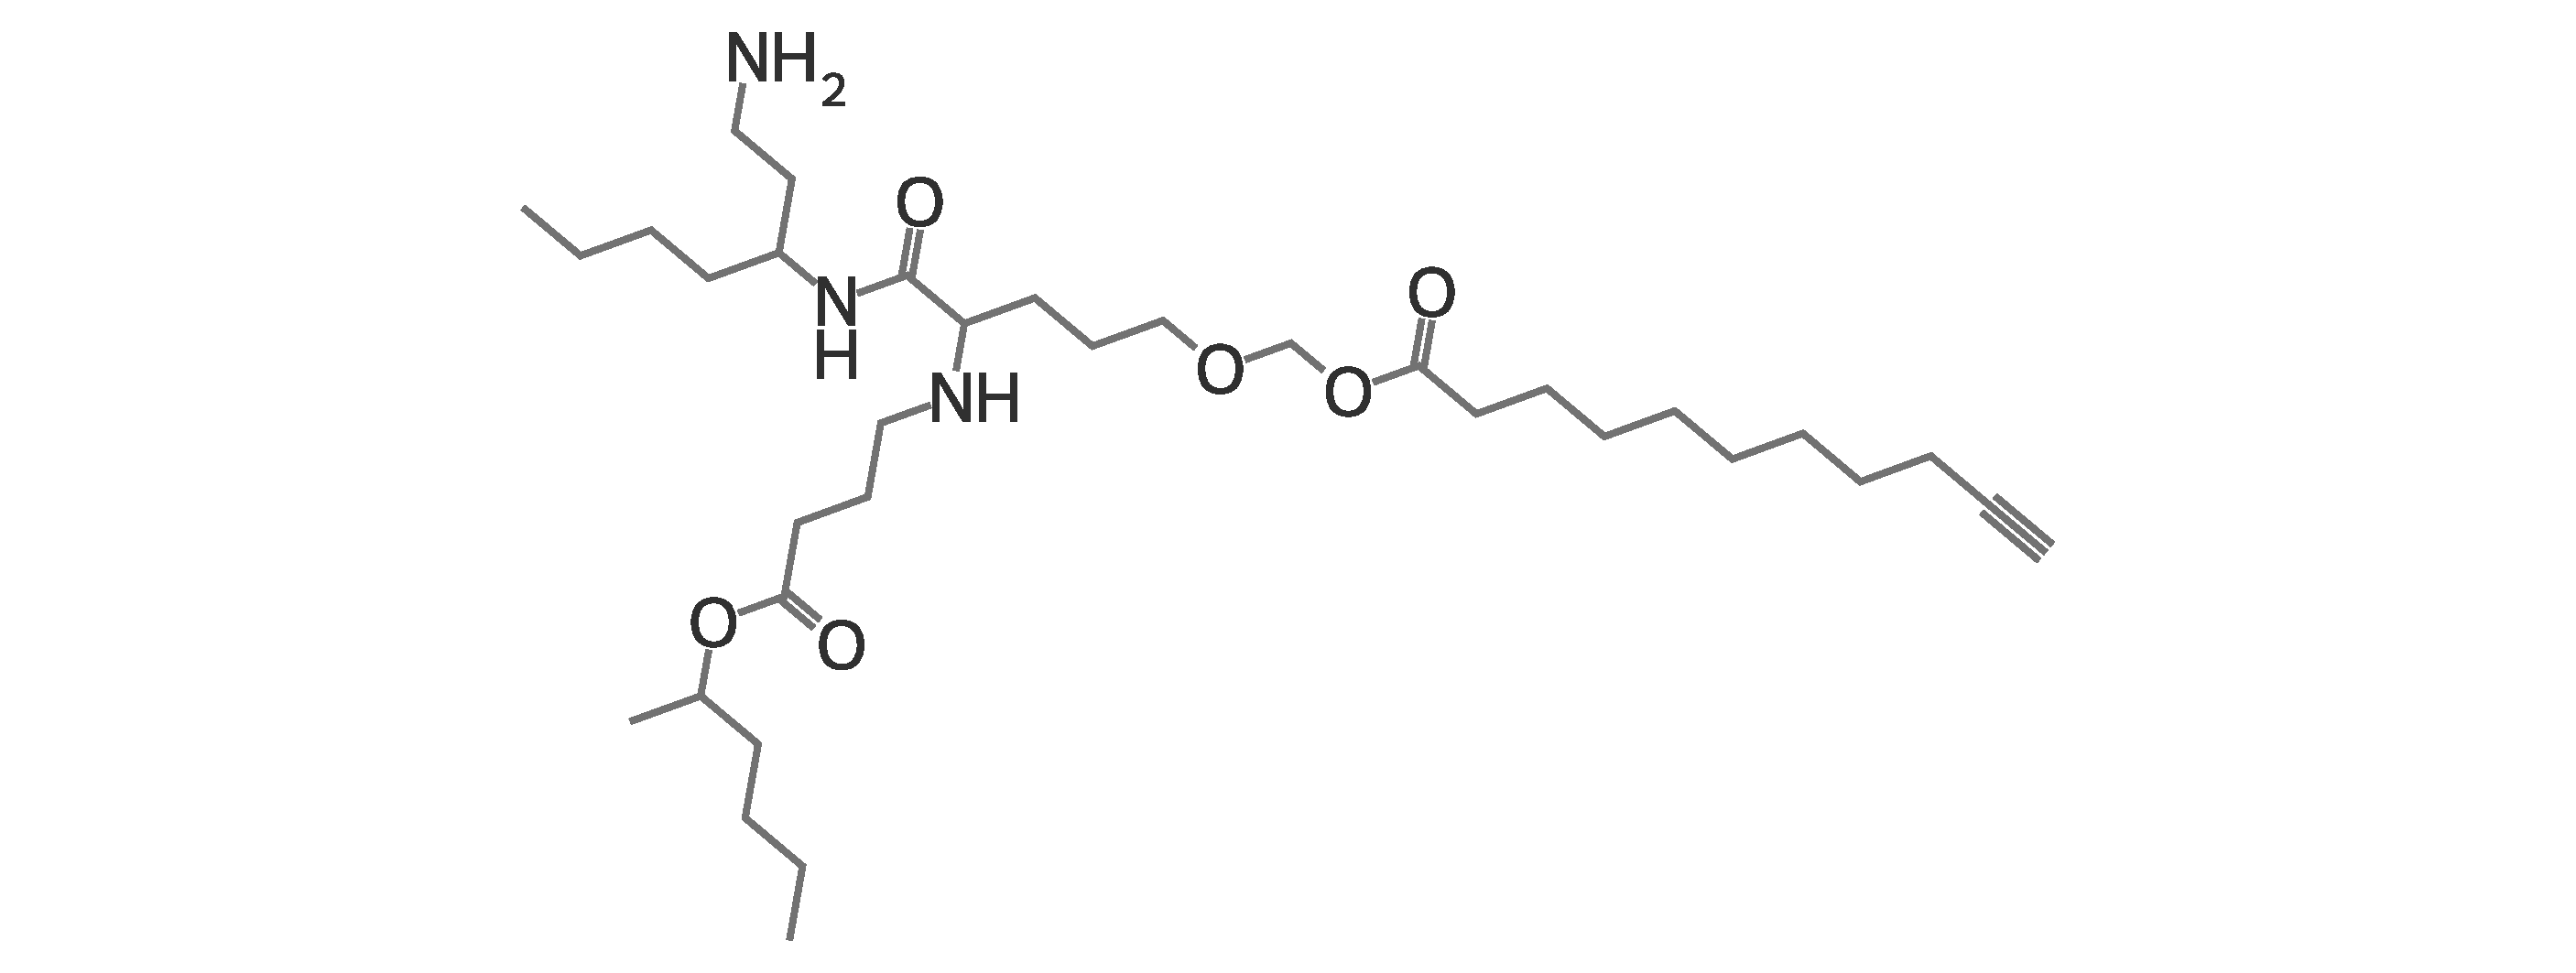
\includegraphics[width=\linewidth,height=\atlasgraphheight,keepaspectratio]{figures/chemical_drawings/atlas_01_2d.pdf}
\par\vspace{\atlassmilesskip}
{\atlassmilesstyle C\#CCCCCCCCCC(=O)OCOCCCC(NCCC\allowbreak{}C(=O)OC(C)CCCC)C(=O)NC(CCN)C\allowbreak{}CCC\par}
\end{minipage}
&
\begin{minipage}[c][\atlasrowheight][c]{\atlasprecursorwidth}
\centering
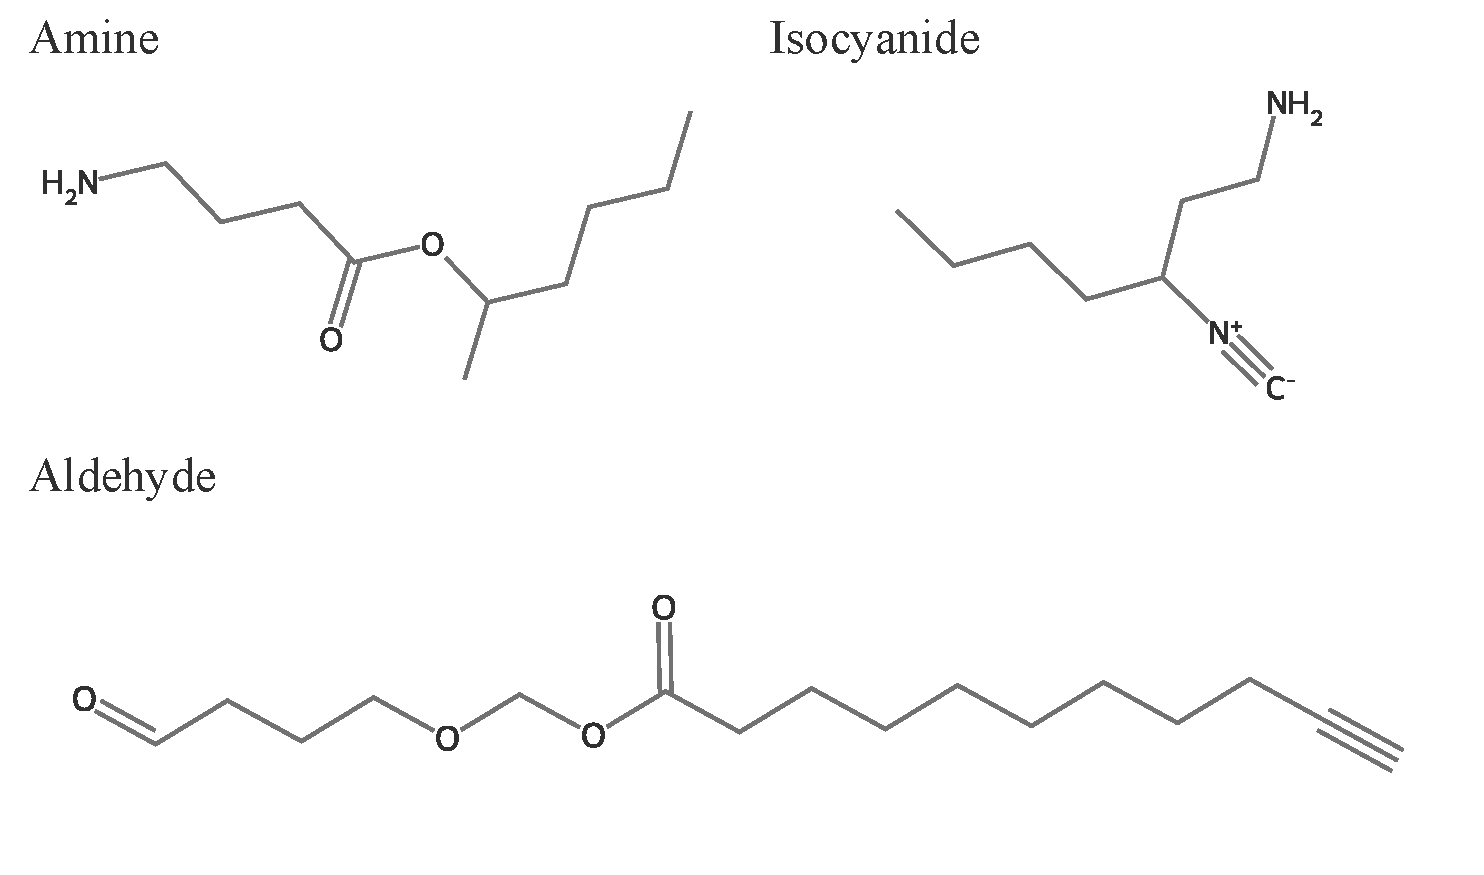
\includegraphics[width=\linewidth,height=\atlasprecursorheight,keepaspectratio]{figures/chemical_drawings/atlas_01_precursors.pdf}
\end{minipage}\\
\atlasrank{2}
&
\begin{minipage}[c][\atlasrowheight][c]{\atlasgraphwidth}
\centering
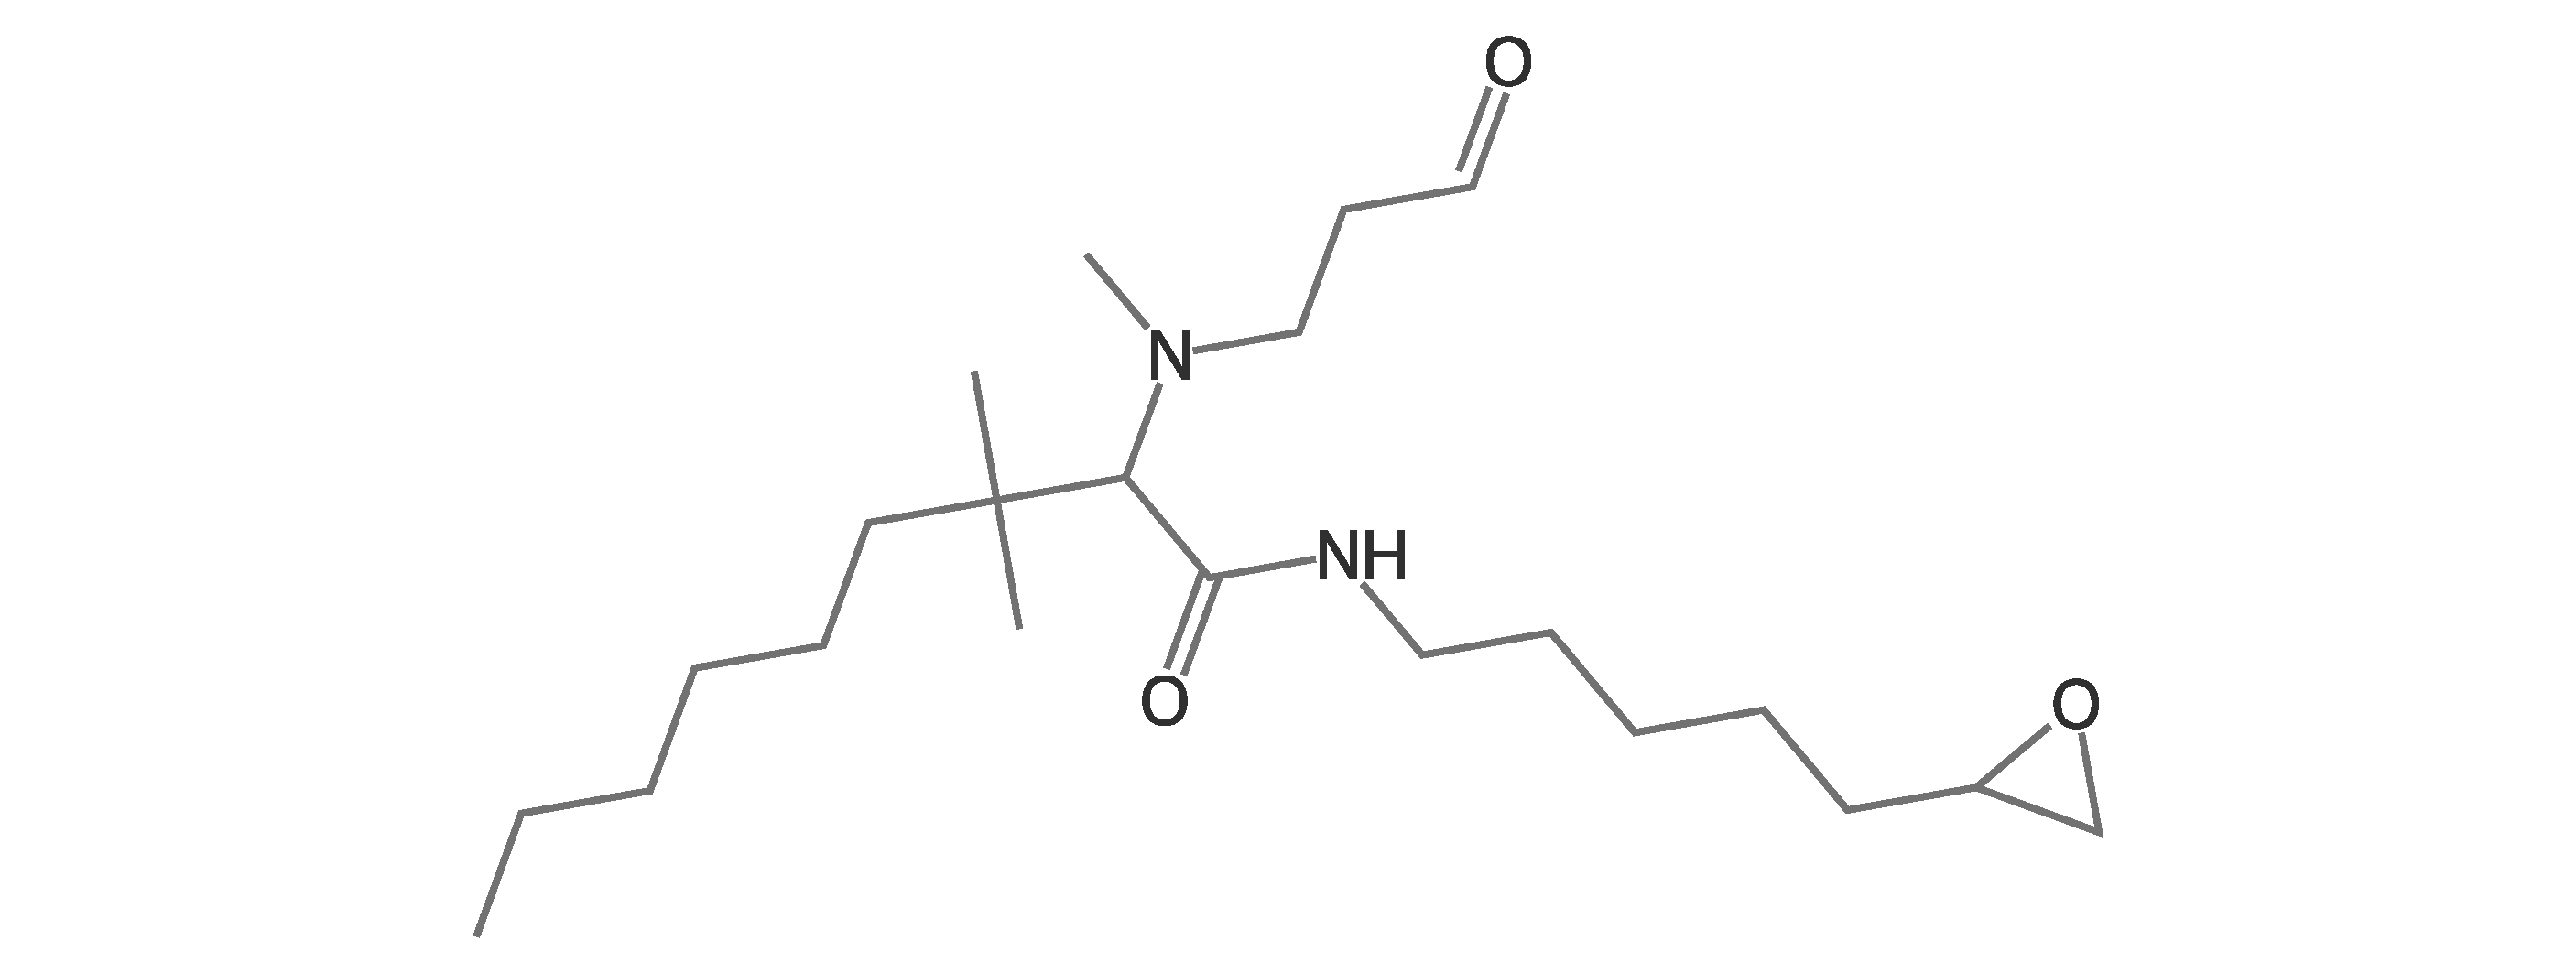
\includegraphics[width=\linewidth,height=\atlasgraphheight,keepaspectratio]{figures/chemical_drawings/atlas_02_2d.pdf}
\par\vspace{\atlassmilesskip}
{\atlassmilesstyle CCCCCCC(C)(C)C(C(=O)NCCCCCC1\allowbreak{}CO1)N(C)CCC=O\par}
\end{minipage}
&
\begin{minipage}[c][\atlasrowheight][c]{\atlasprecursorwidth}
\centering
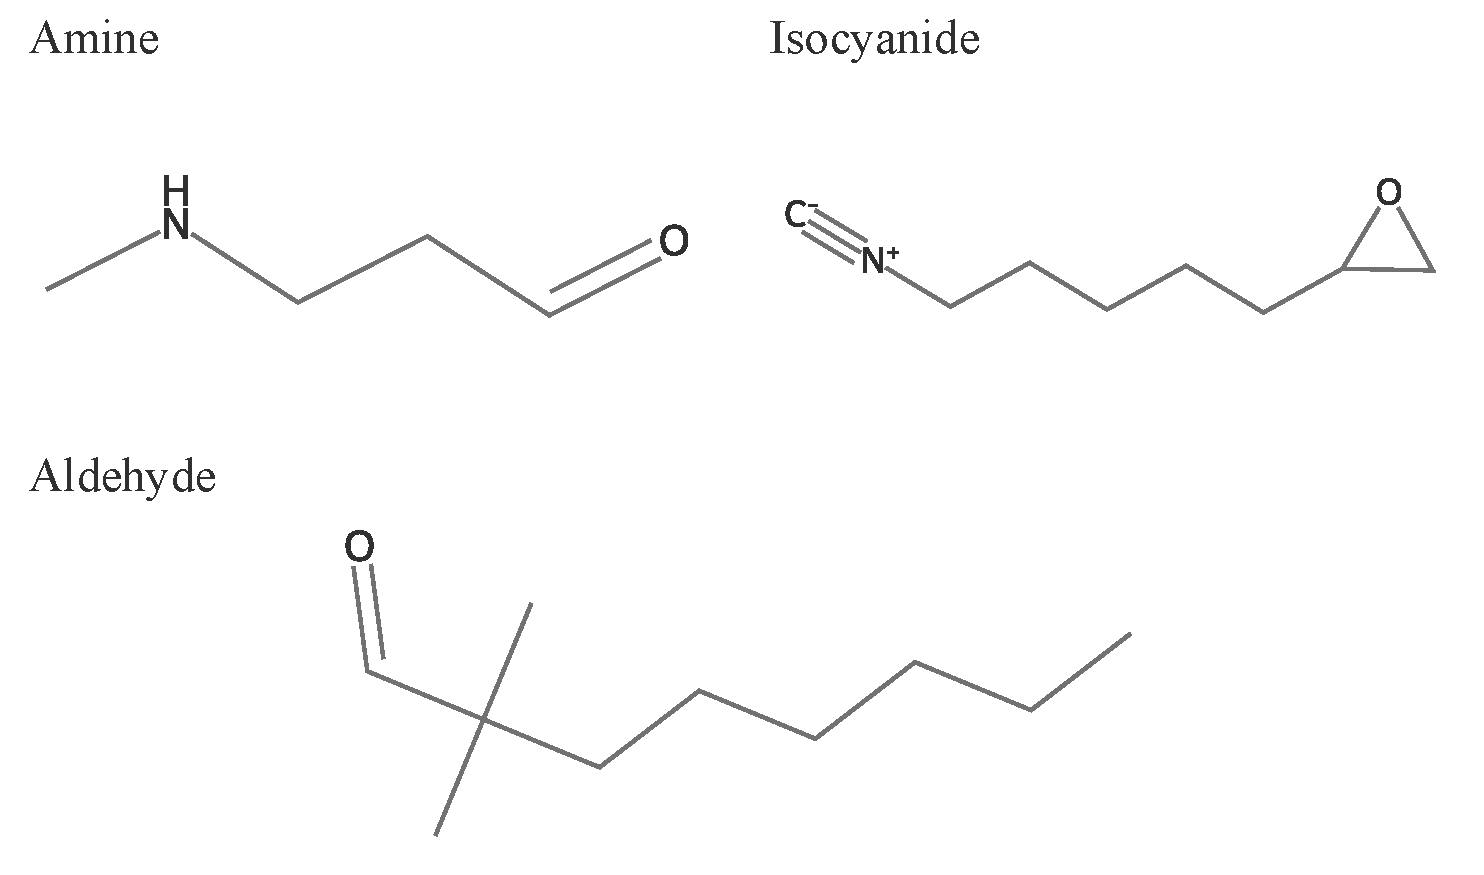
\includegraphics[width=\linewidth,height=\atlasprecursorheight,keepaspectratio]{figures/chemical_drawings/atlas_02_precursors.pdf}
\end{minipage}\\
\atlasrank{3}
&
\begin{minipage}[c][\atlasrowheight][c]{\atlasgraphwidth}
\centering
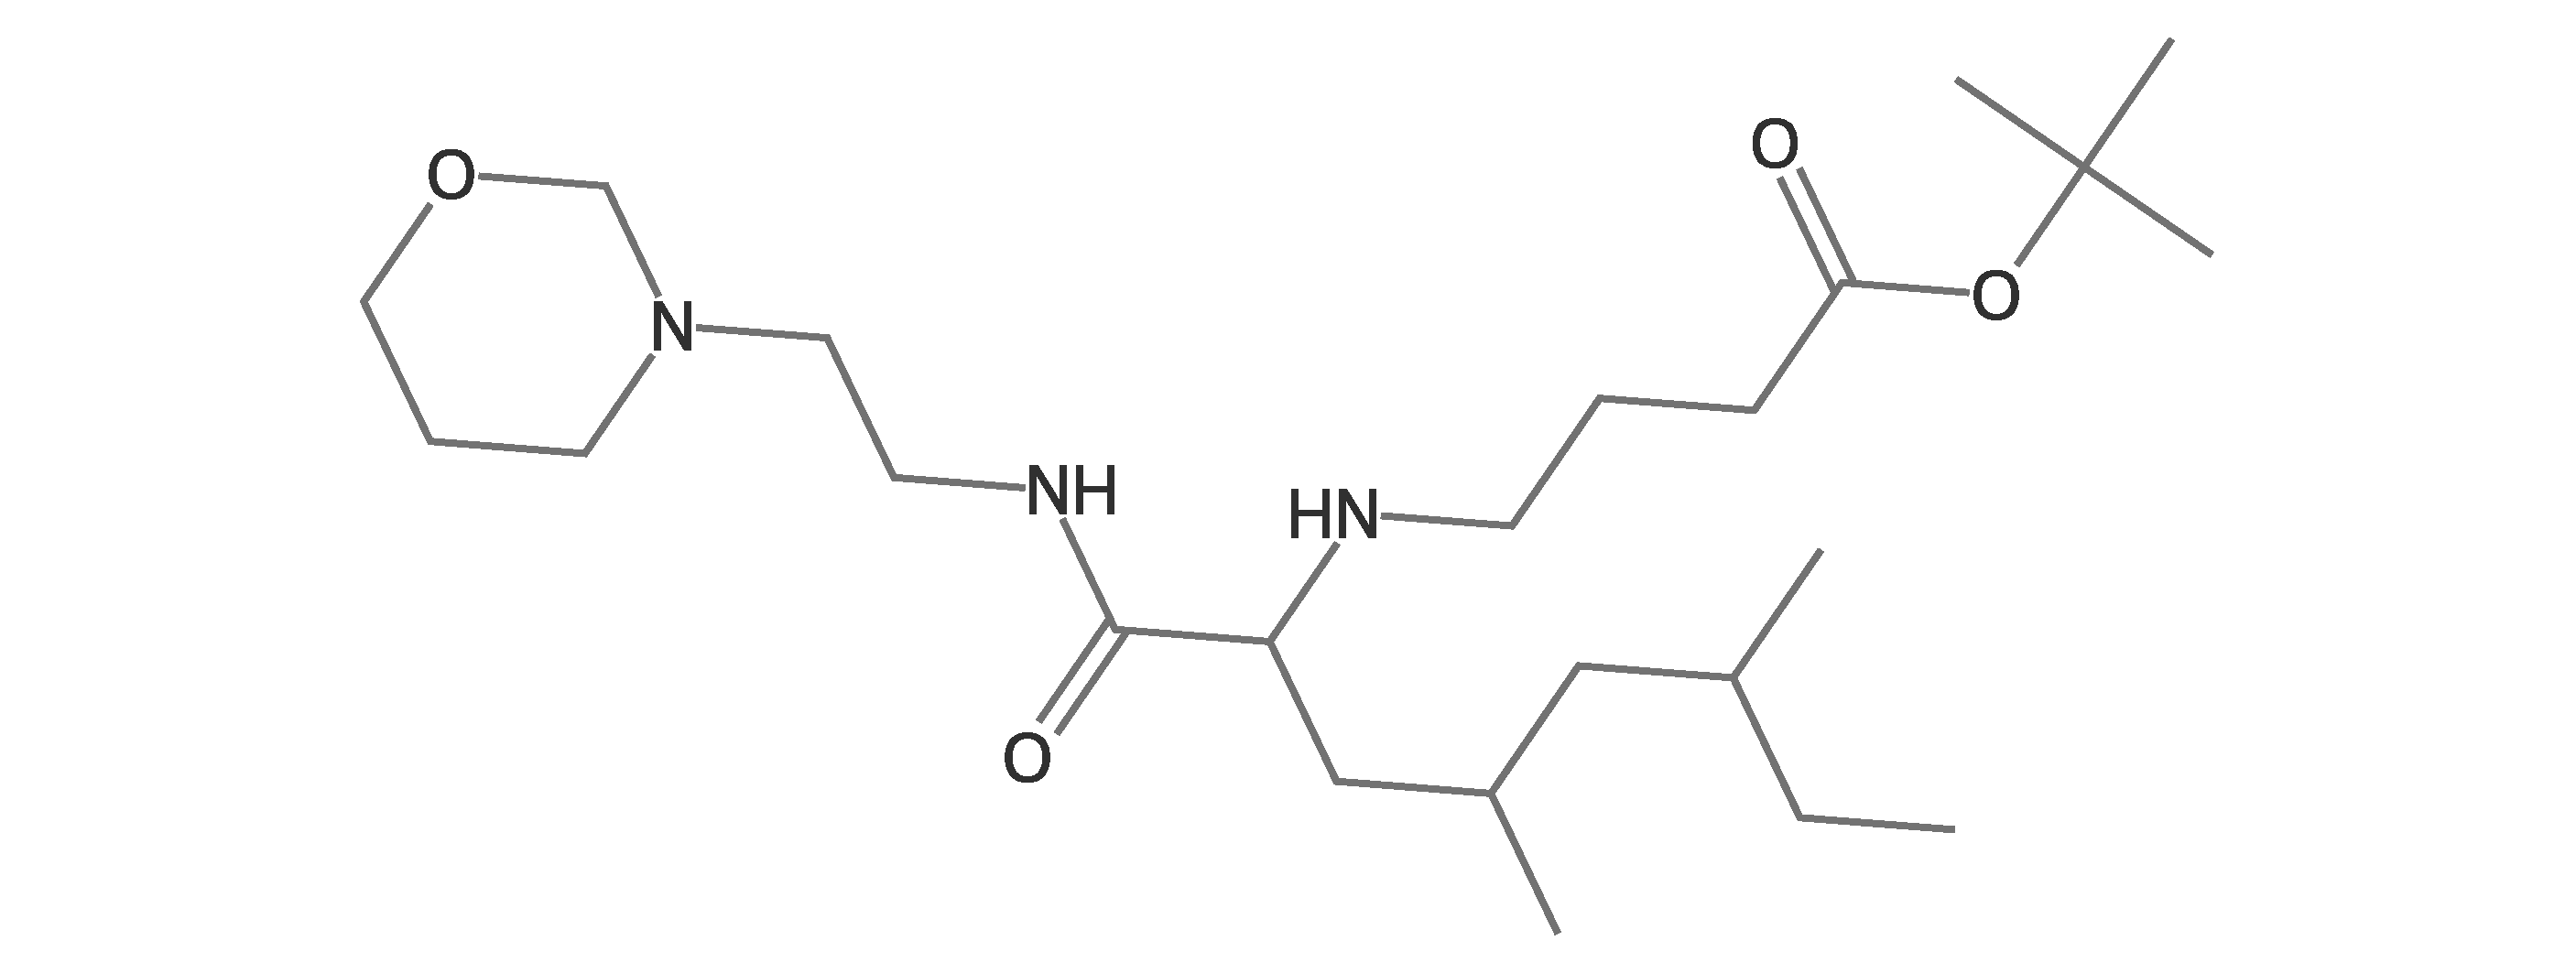
\includegraphics[width=\linewidth,height=\atlasgraphheight,keepaspectratio]{figures/chemical_drawings/atlas_03_2d.pdf}
\par\vspace{\atlassmilesskip}
{\atlassmilesstyle CCC(C)CC(C)CC(NCCCC(=O)OC(C)\allowbreak{}(C)C)C(=O)NCCN1CCCOC1\par}
\end{minipage}
&
\begin{minipage}[c][\atlasrowheight][c]{\atlasprecursorwidth}
\centering
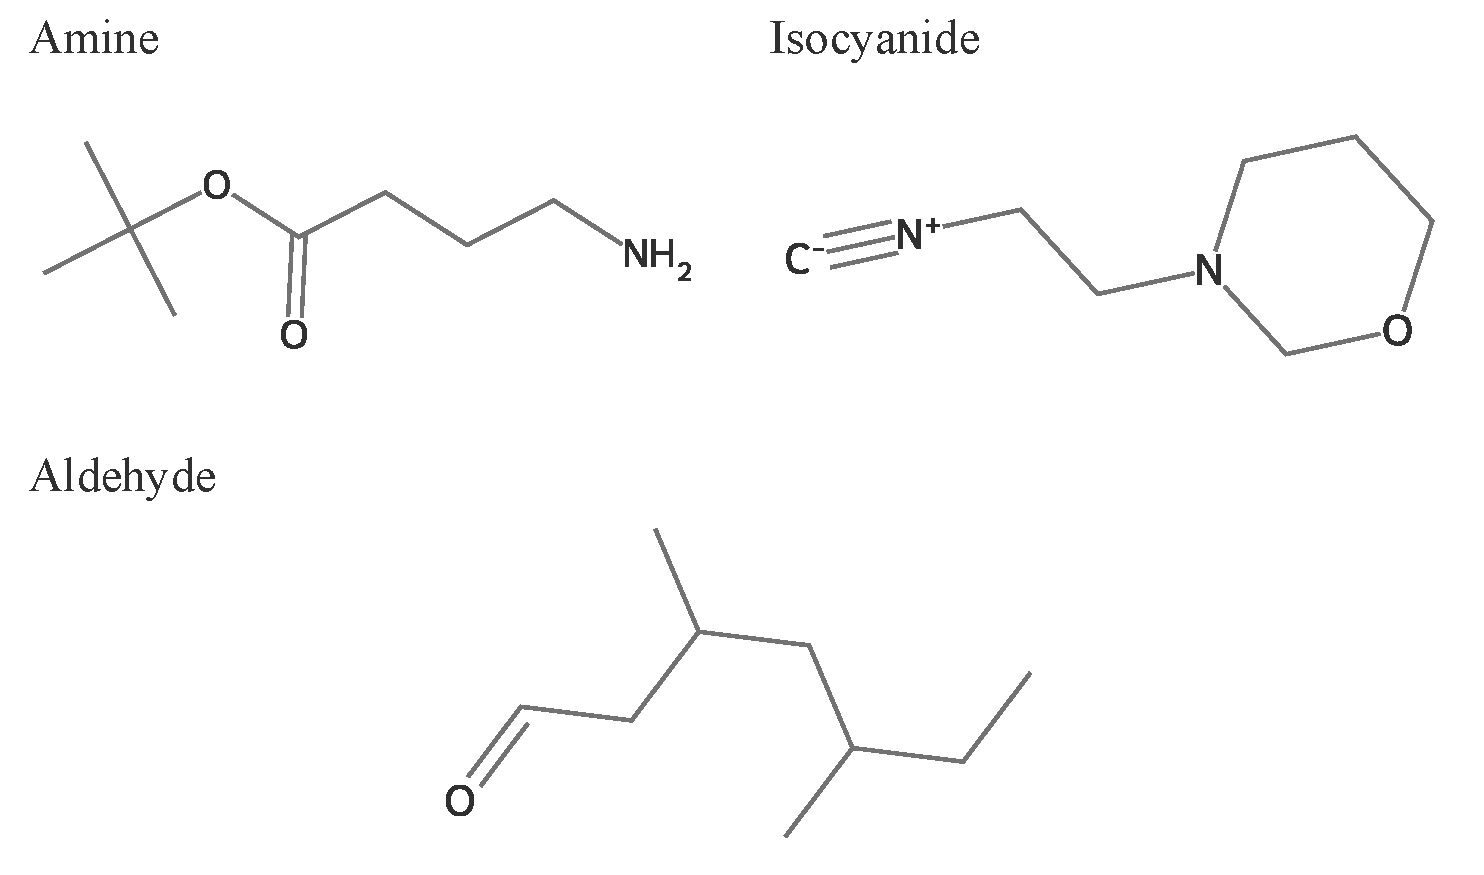
\includegraphics[width=\linewidth,height=\atlasprecursorheight,keepaspectratio]{figures/chemical_drawings/atlas_03_precursors.pdf}
\end{minipage}\\
\atlasrank{4}
&
\begin{minipage}[c][\atlasrowheight][c]{\atlasgraphwidth}
\centering
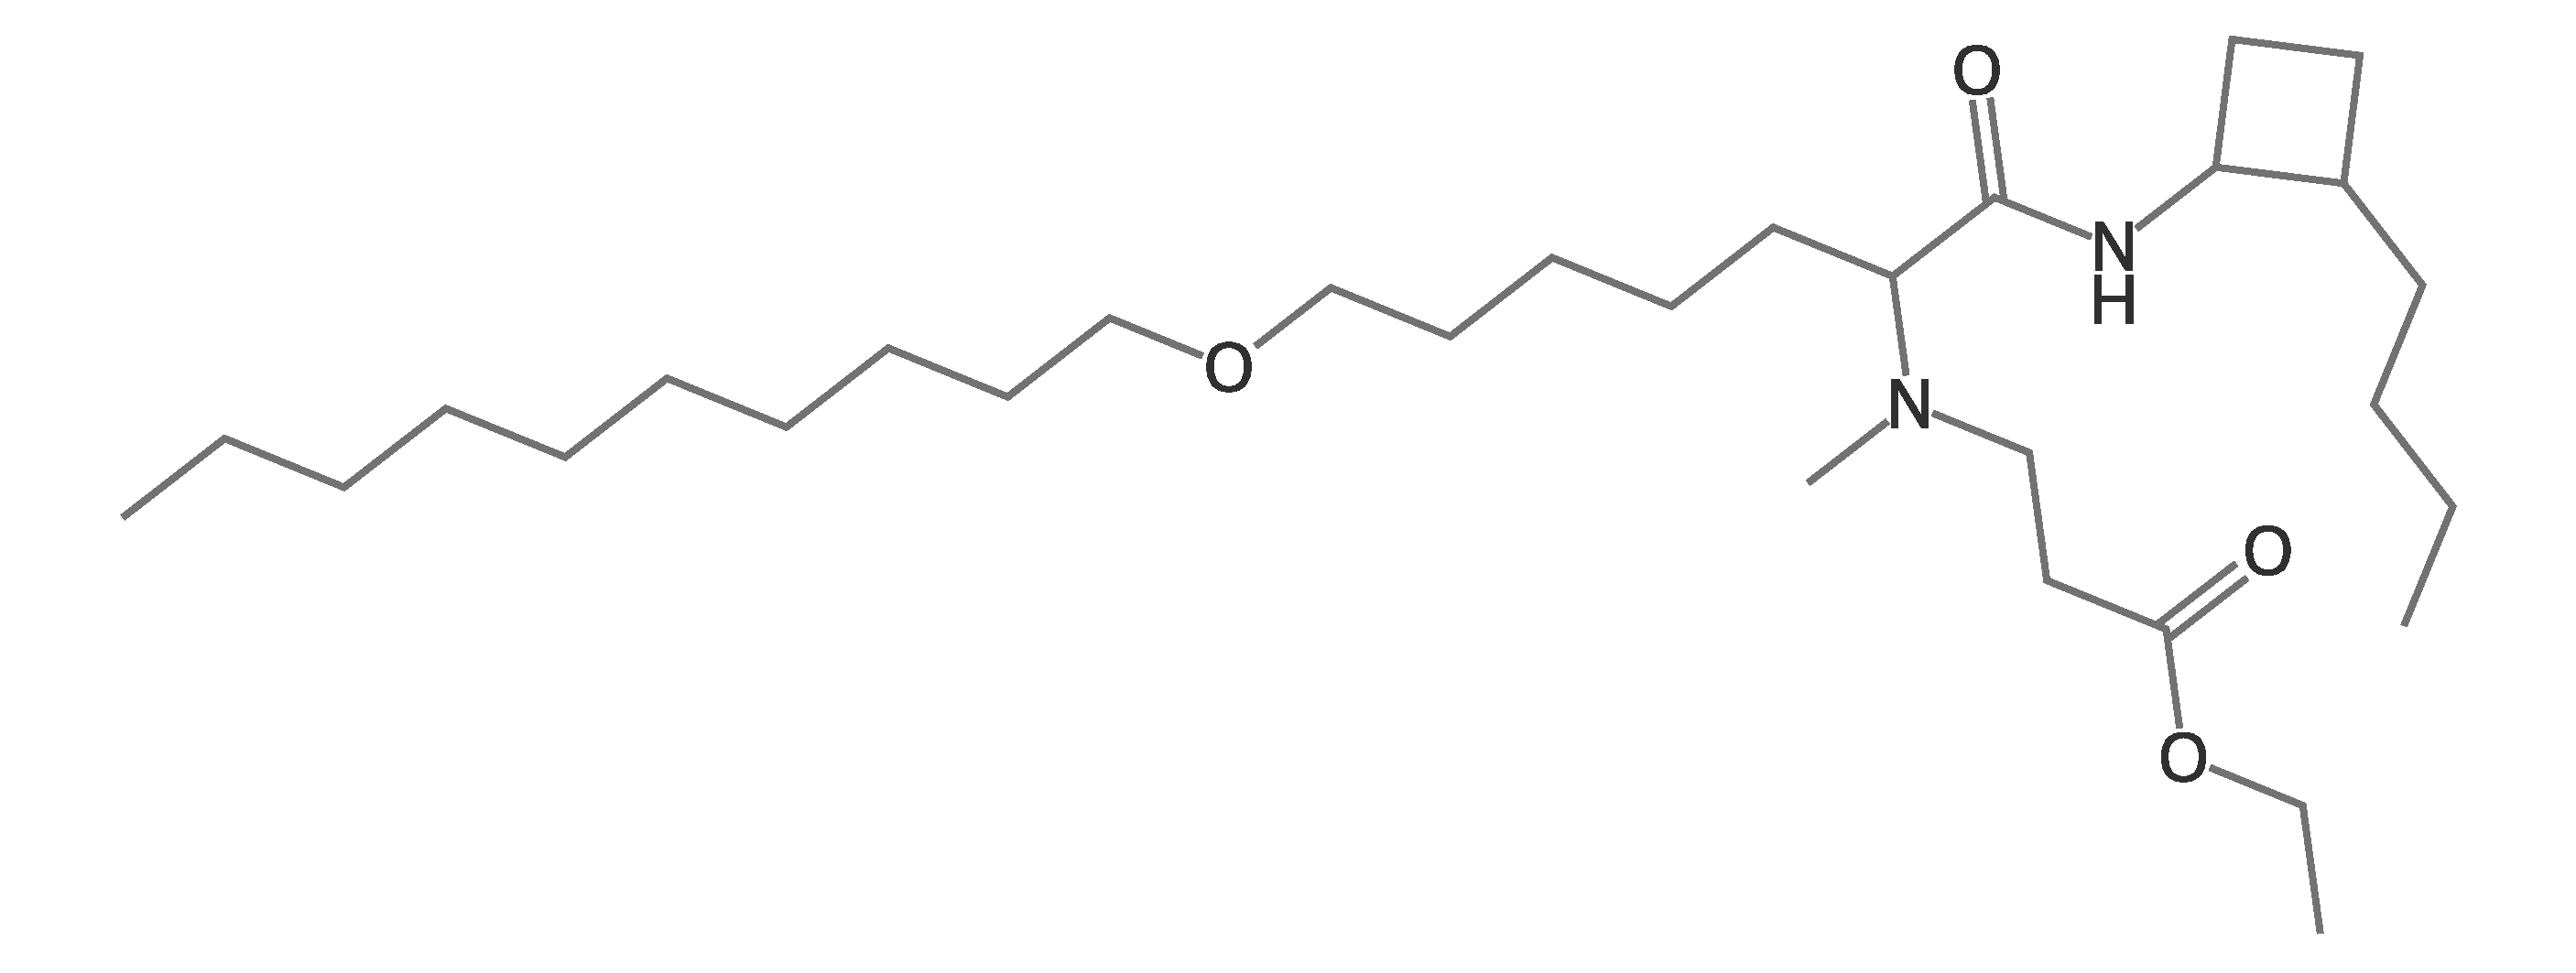
\includegraphics[width=\linewidth,height=\atlasgraphheight,keepaspectratio]{figures/chemical_drawings/atlas_04_2d.pdf}
\par\vspace{\atlassmilesskip}
{\atlassmilesstyle CCCCCCCCCCOCCCCCC(C(=O)NC1CC\allowbreak{}C1CCCC)N(C)CCC(=O)OCC\par}
\end{minipage}
&
\begin{minipage}[c][\atlasrowheight][c]{\atlasprecursorwidth}
\centering
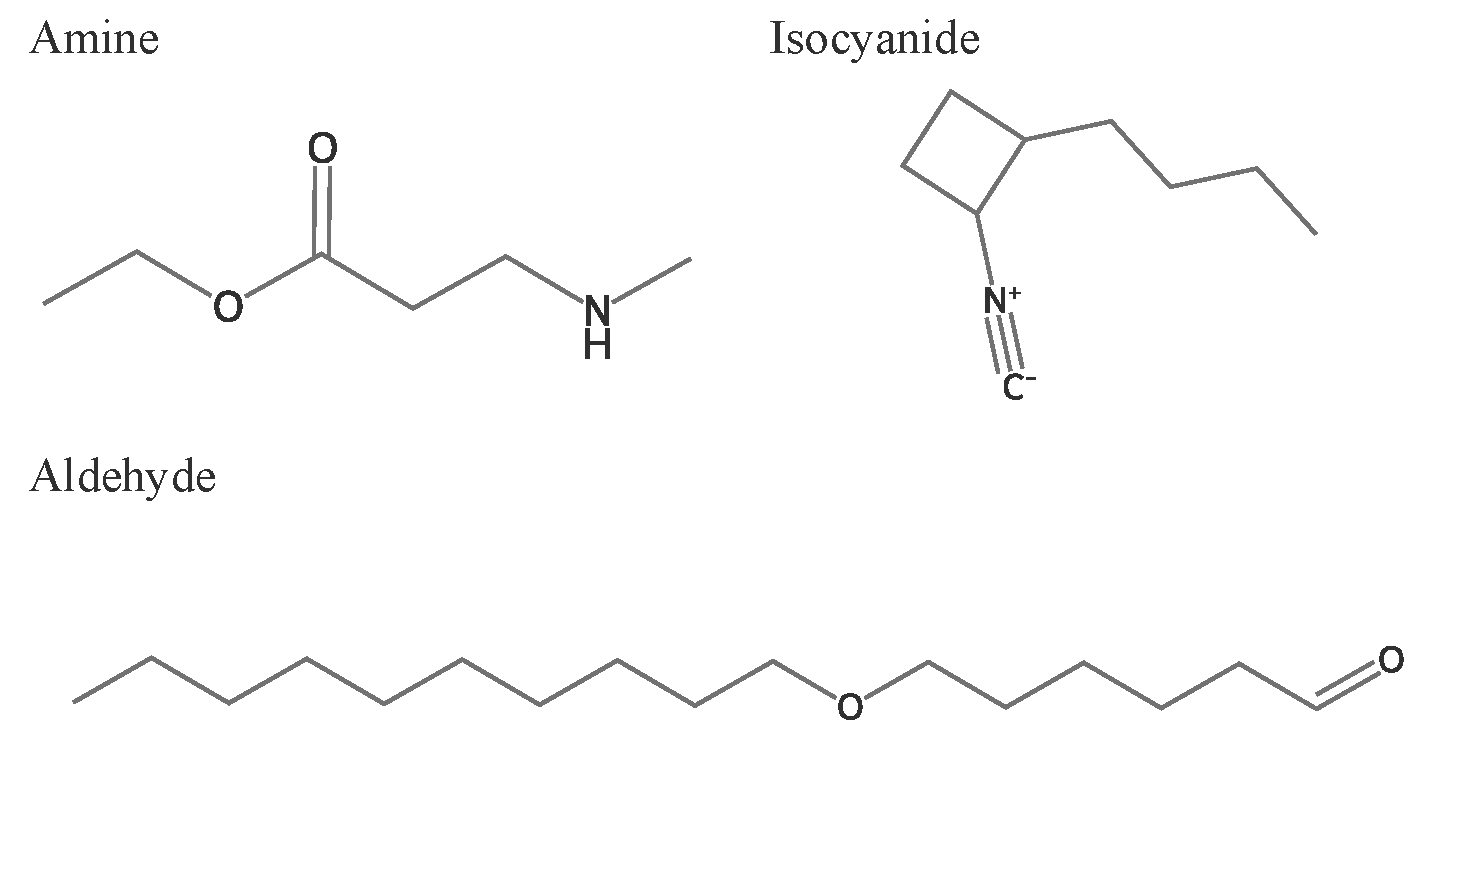
\includegraphics[width=\linewidth,height=\atlasprecursorheight,keepaspectratio]{figures/chemical_drawings/atlas_04_precursors.pdf}
\end{minipage}\\
\atlasrank{5}
&
\begin{minipage}[c][\atlasrowheight][c]{\atlasgraphwidth}
\centering
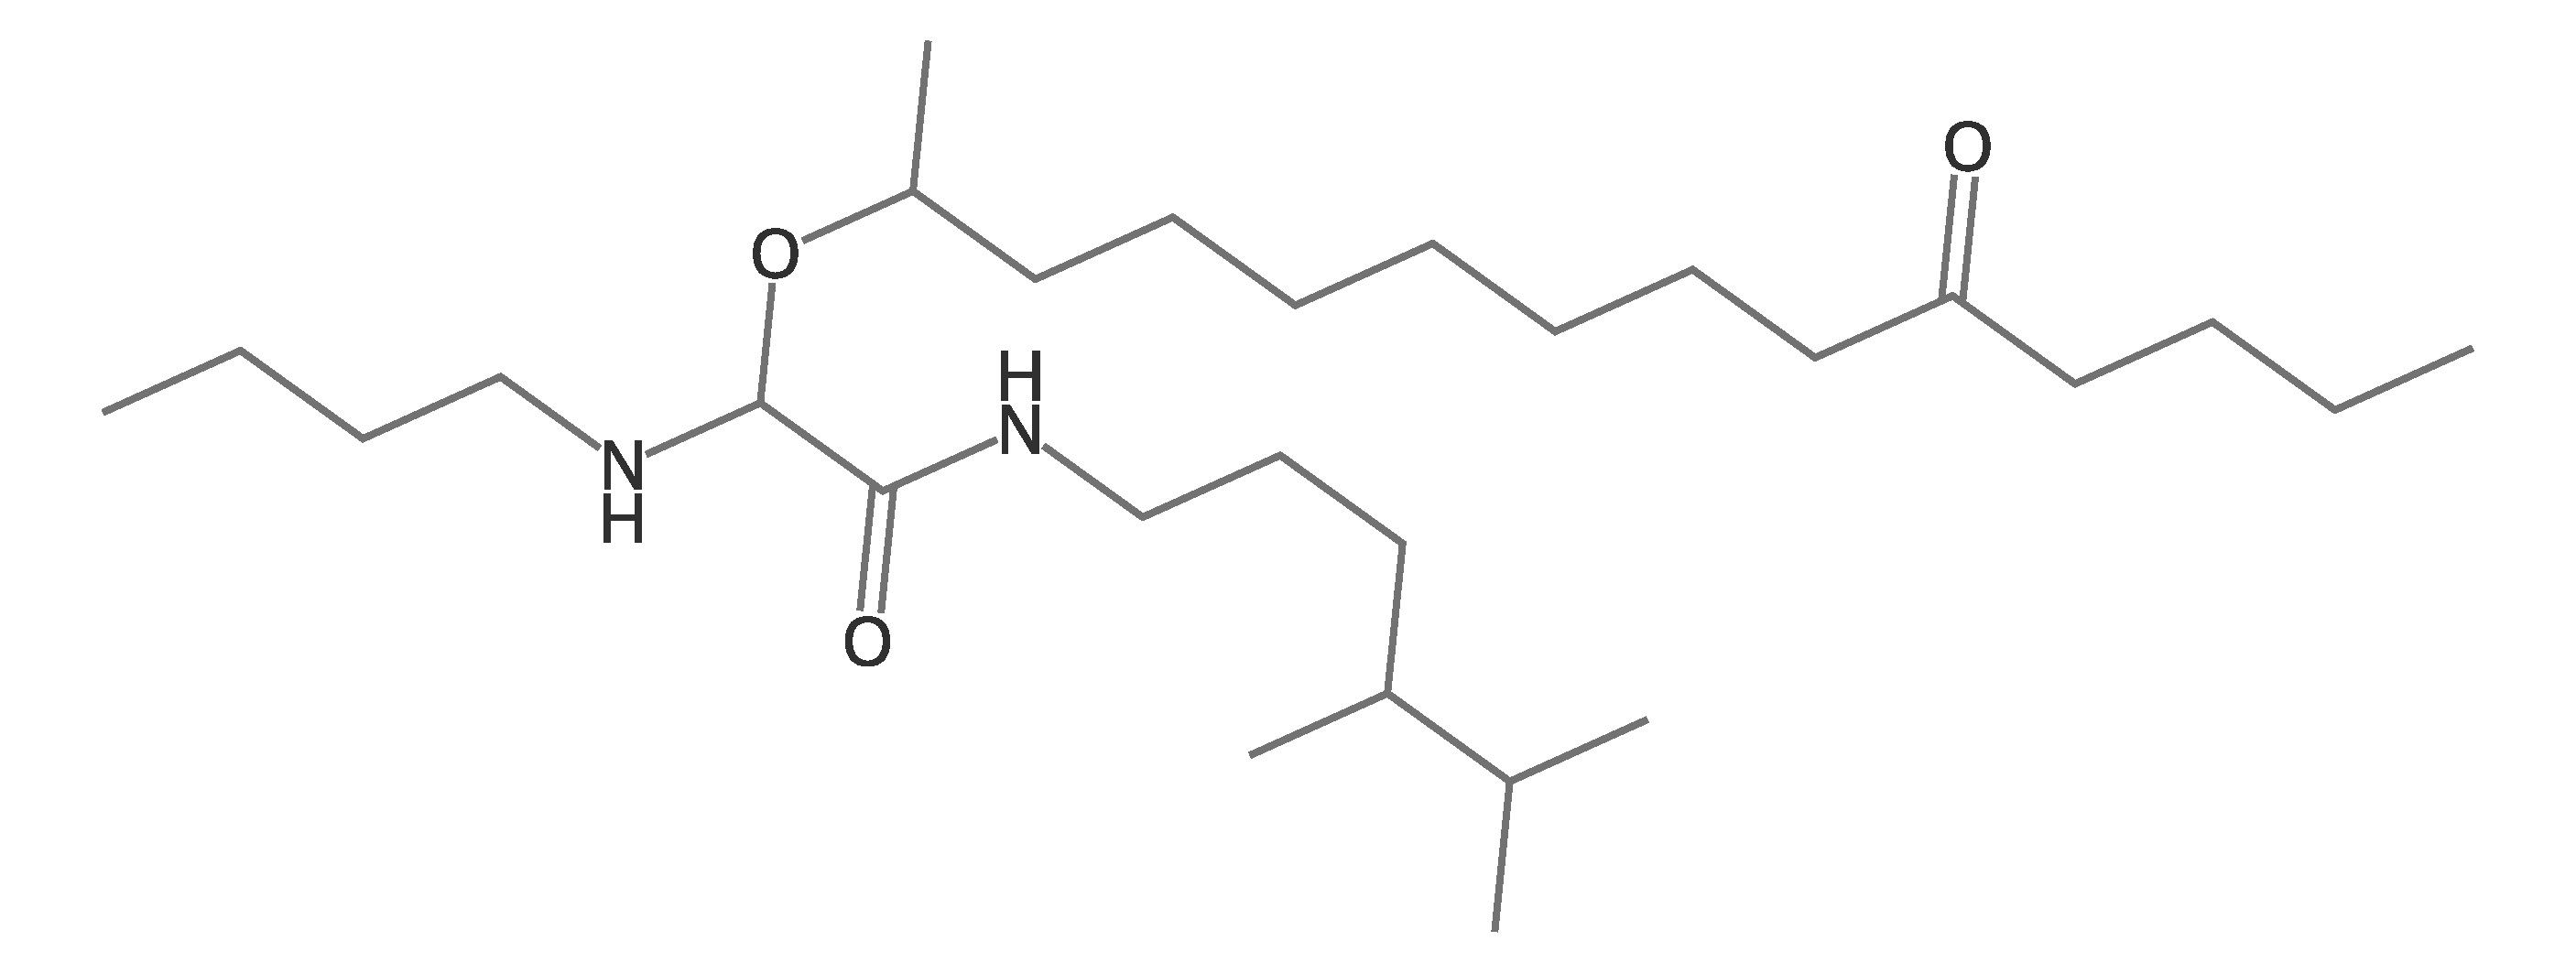
\includegraphics[width=\linewidth,height=\atlasgraphheight,keepaspectratio]{figures/chemical_drawings/atlas_05_2d.pdf}
\par\vspace{\atlassmilesskip}
{\atlassmilesstyle CCCCNC(OC(C)CCCCCCCC(=O)CCCC\allowbreak{})C(=O)NCCCC(C)C(C)C\par}
\end{minipage}
&
\begin{minipage}[c][\atlasrowheight][c]{\atlasprecursorwidth}
\centering
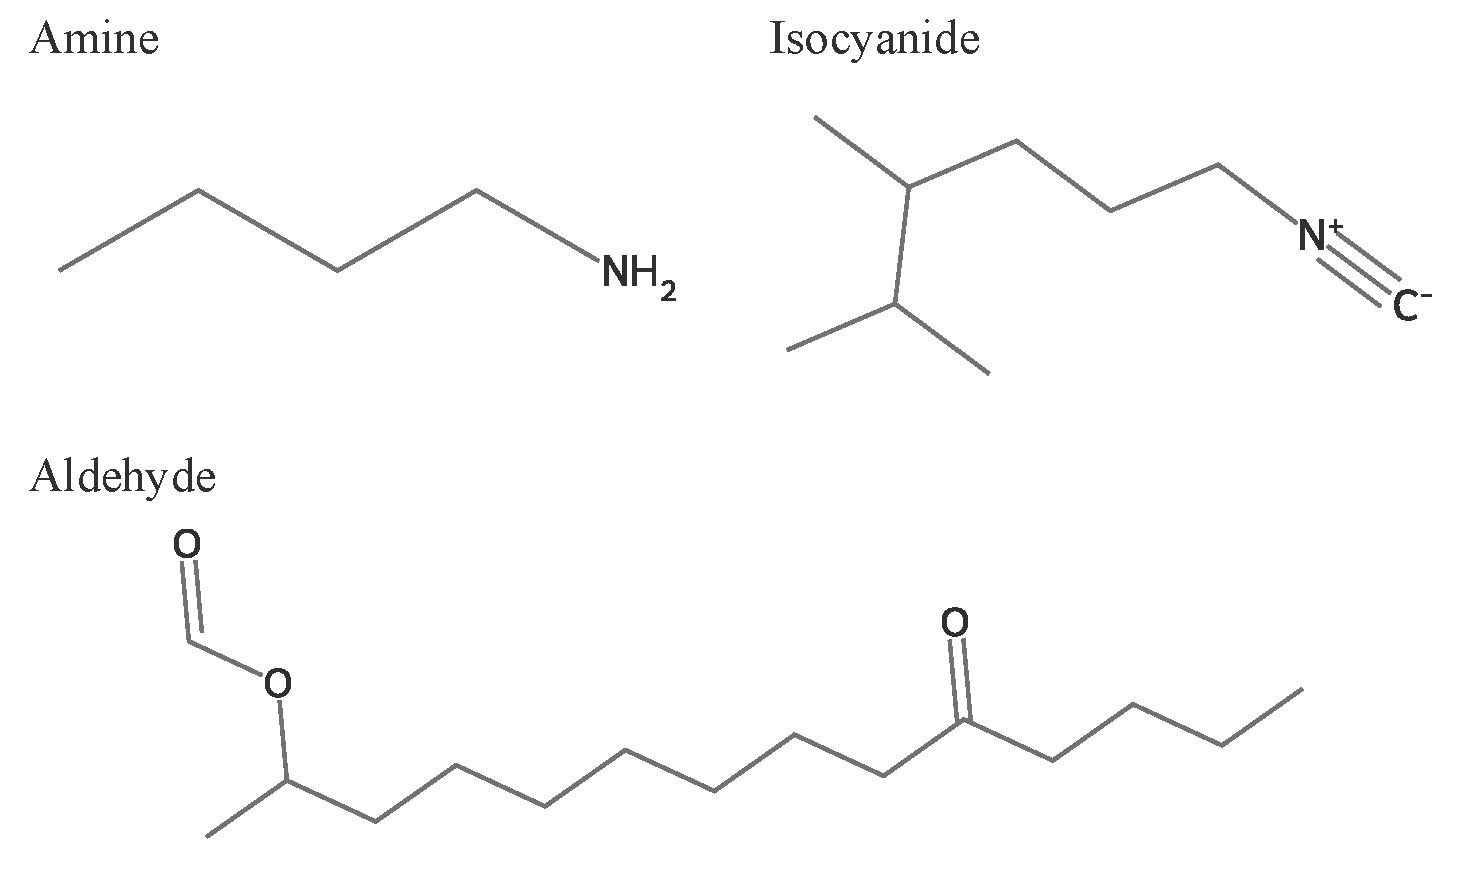
\includegraphics[width=\linewidth,height=\atlasprecursorheight,keepaspectratio]{figures/chemical_drawings/atlas_05_precursors.pdf}
\end{minipage}\\
\atlasrank{6}
&
\begin{minipage}[c][\atlasrowheight][c]{\atlasgraphwidth}
\centering
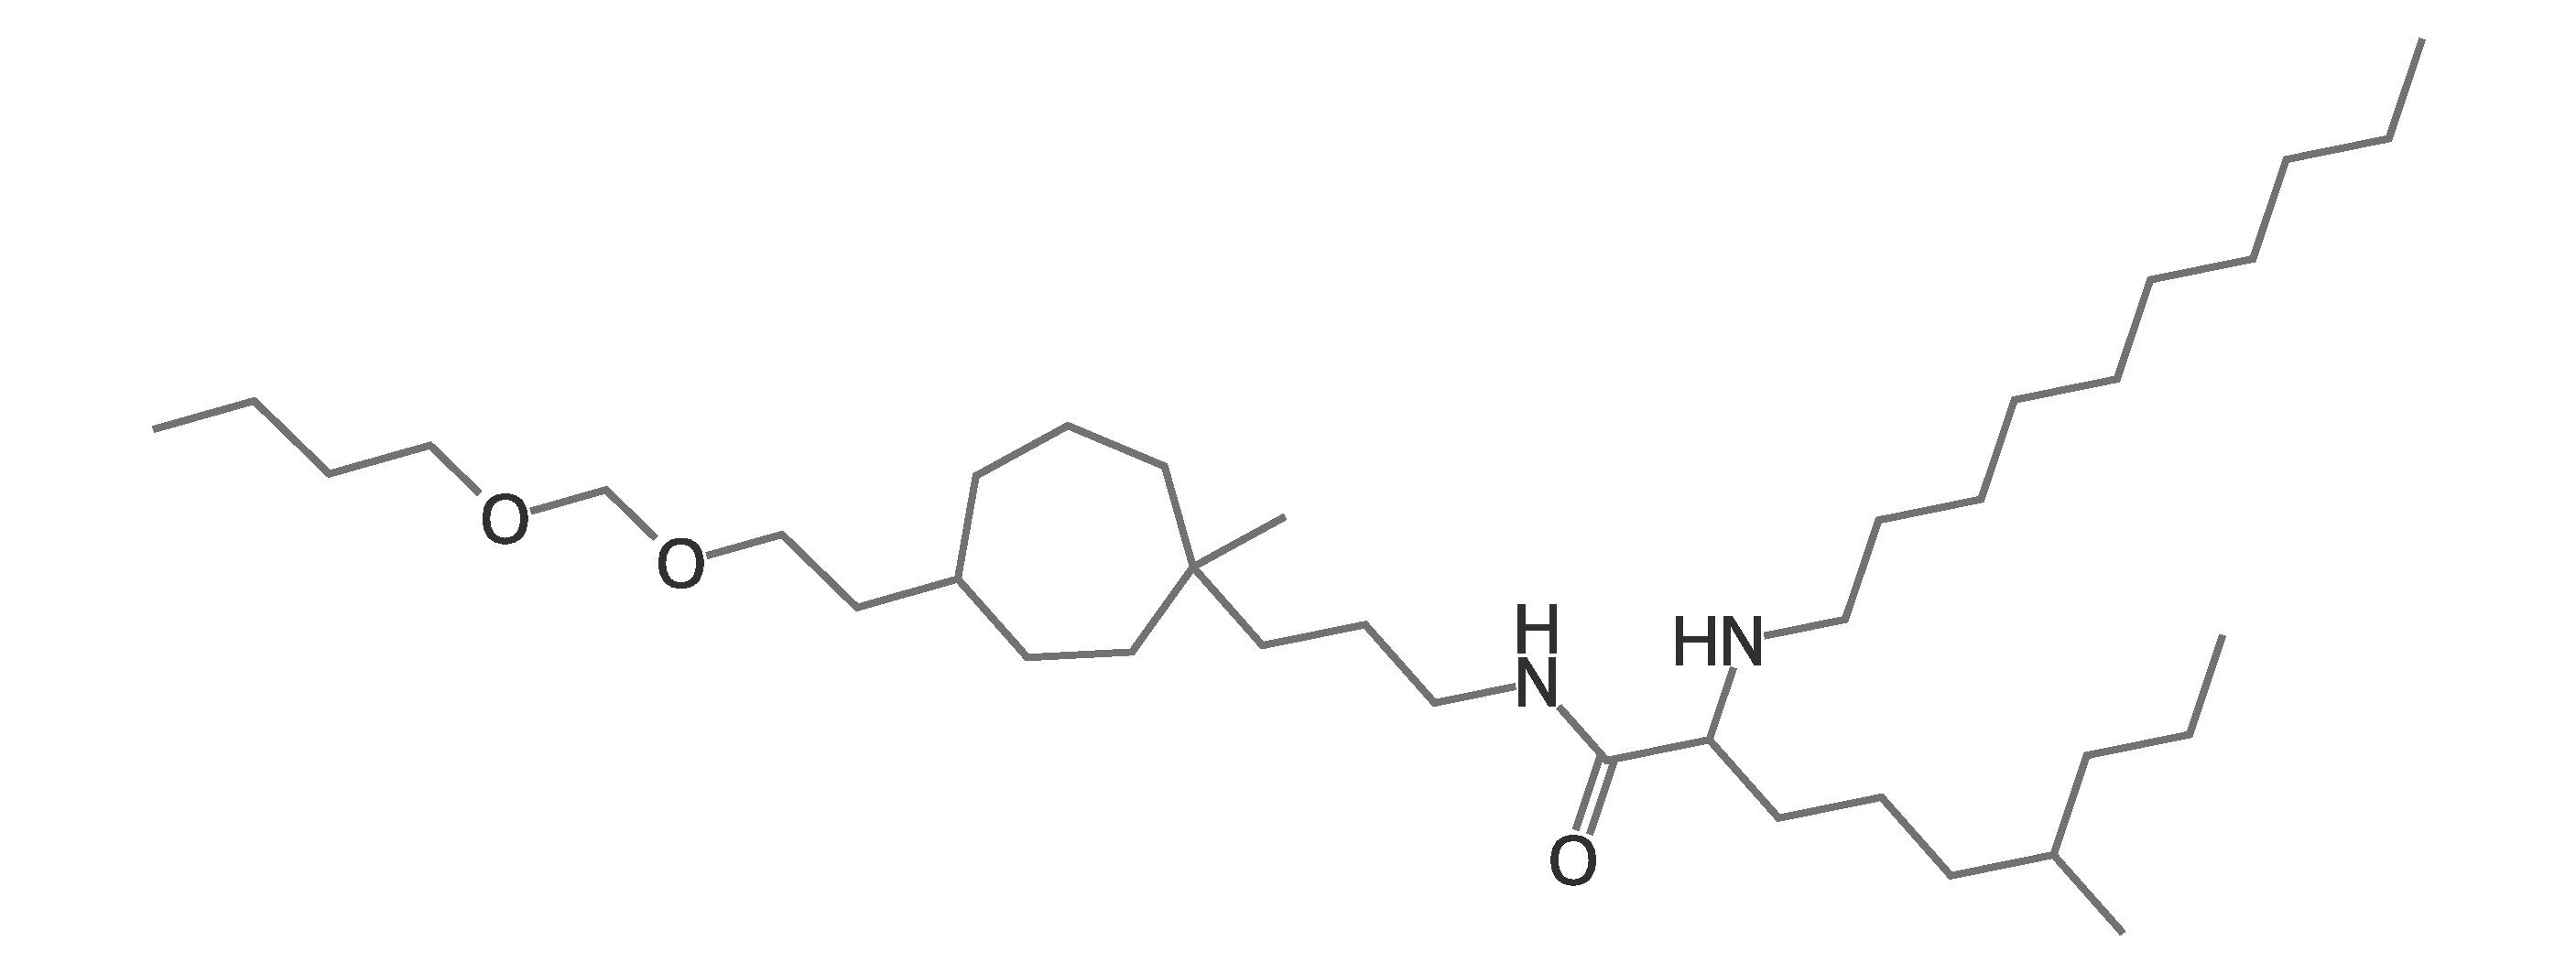
\includegraphics[width=\linewidth,height=\atlasgraphheight,keepaspectratio]{figures/chemical_drawings/atlas_06_2d.pdf}
\par\vspace{\atlassmilesskip}
{\atlassmilesstyle CCCCCCCCCCNC(CCCC(C)CCC)C(=O\allowbreak{})NCCCC1(C)CCCC(CCOCOCCCC)CC1\par}
\end{minipage}
&
\begin{minipage}[c][\atlasrowheight][c]{\atlasprecursorwidth}
\centering
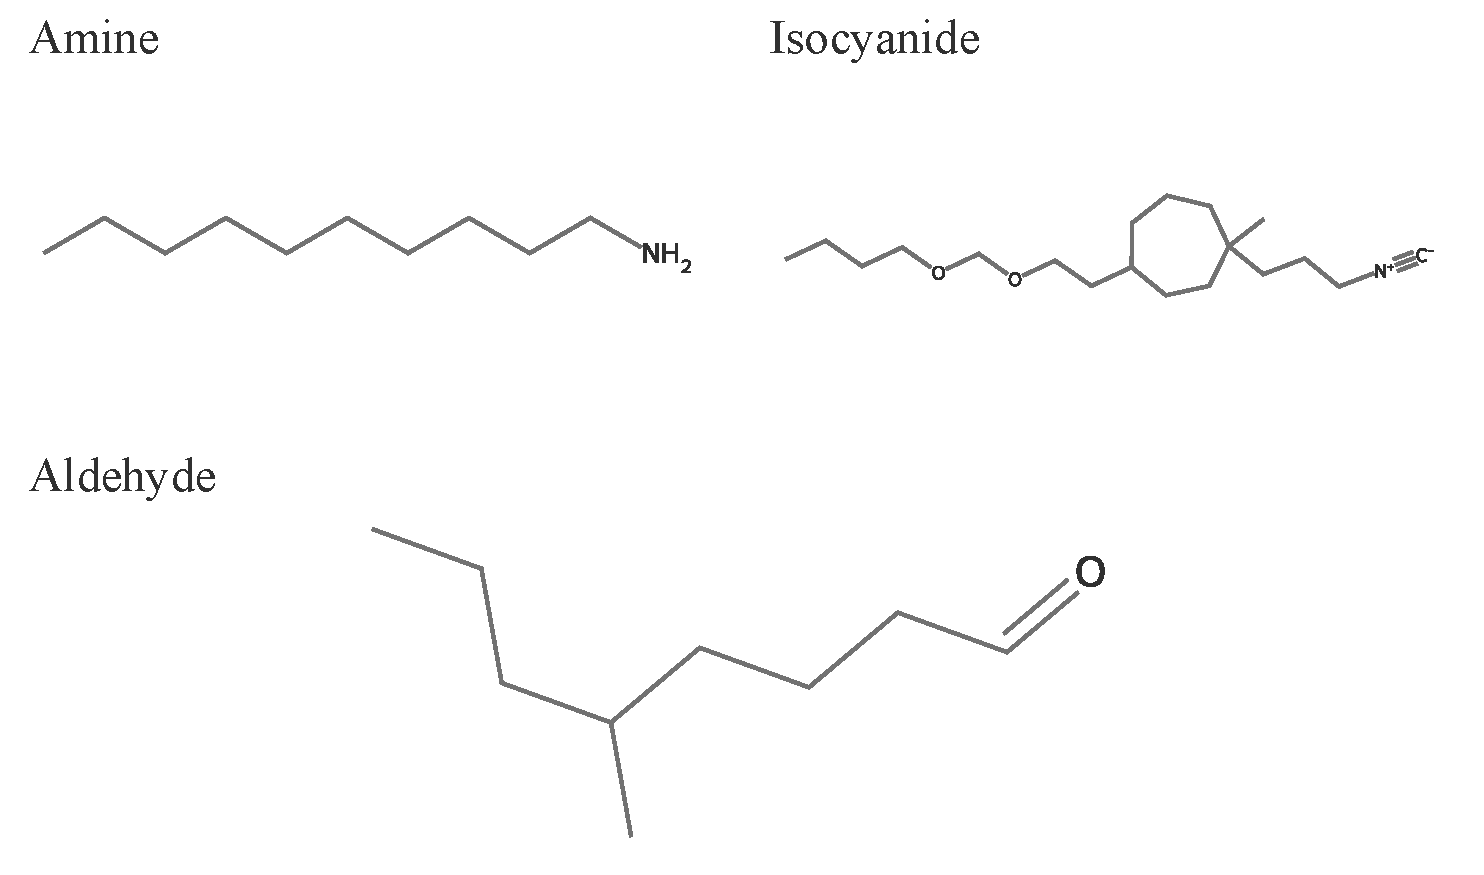
\includegraphics[width=\linewidth,height=\atlasprecursorheight,keepaspectratio]{figures/chemical_drawings/atlas_06_precursors.pdf}
\end{minipage}\\
\atlasrank{7}
&
\begin{minipage}[c][\atlasrowheight][c]{\atlasgraphwidth}
\centering
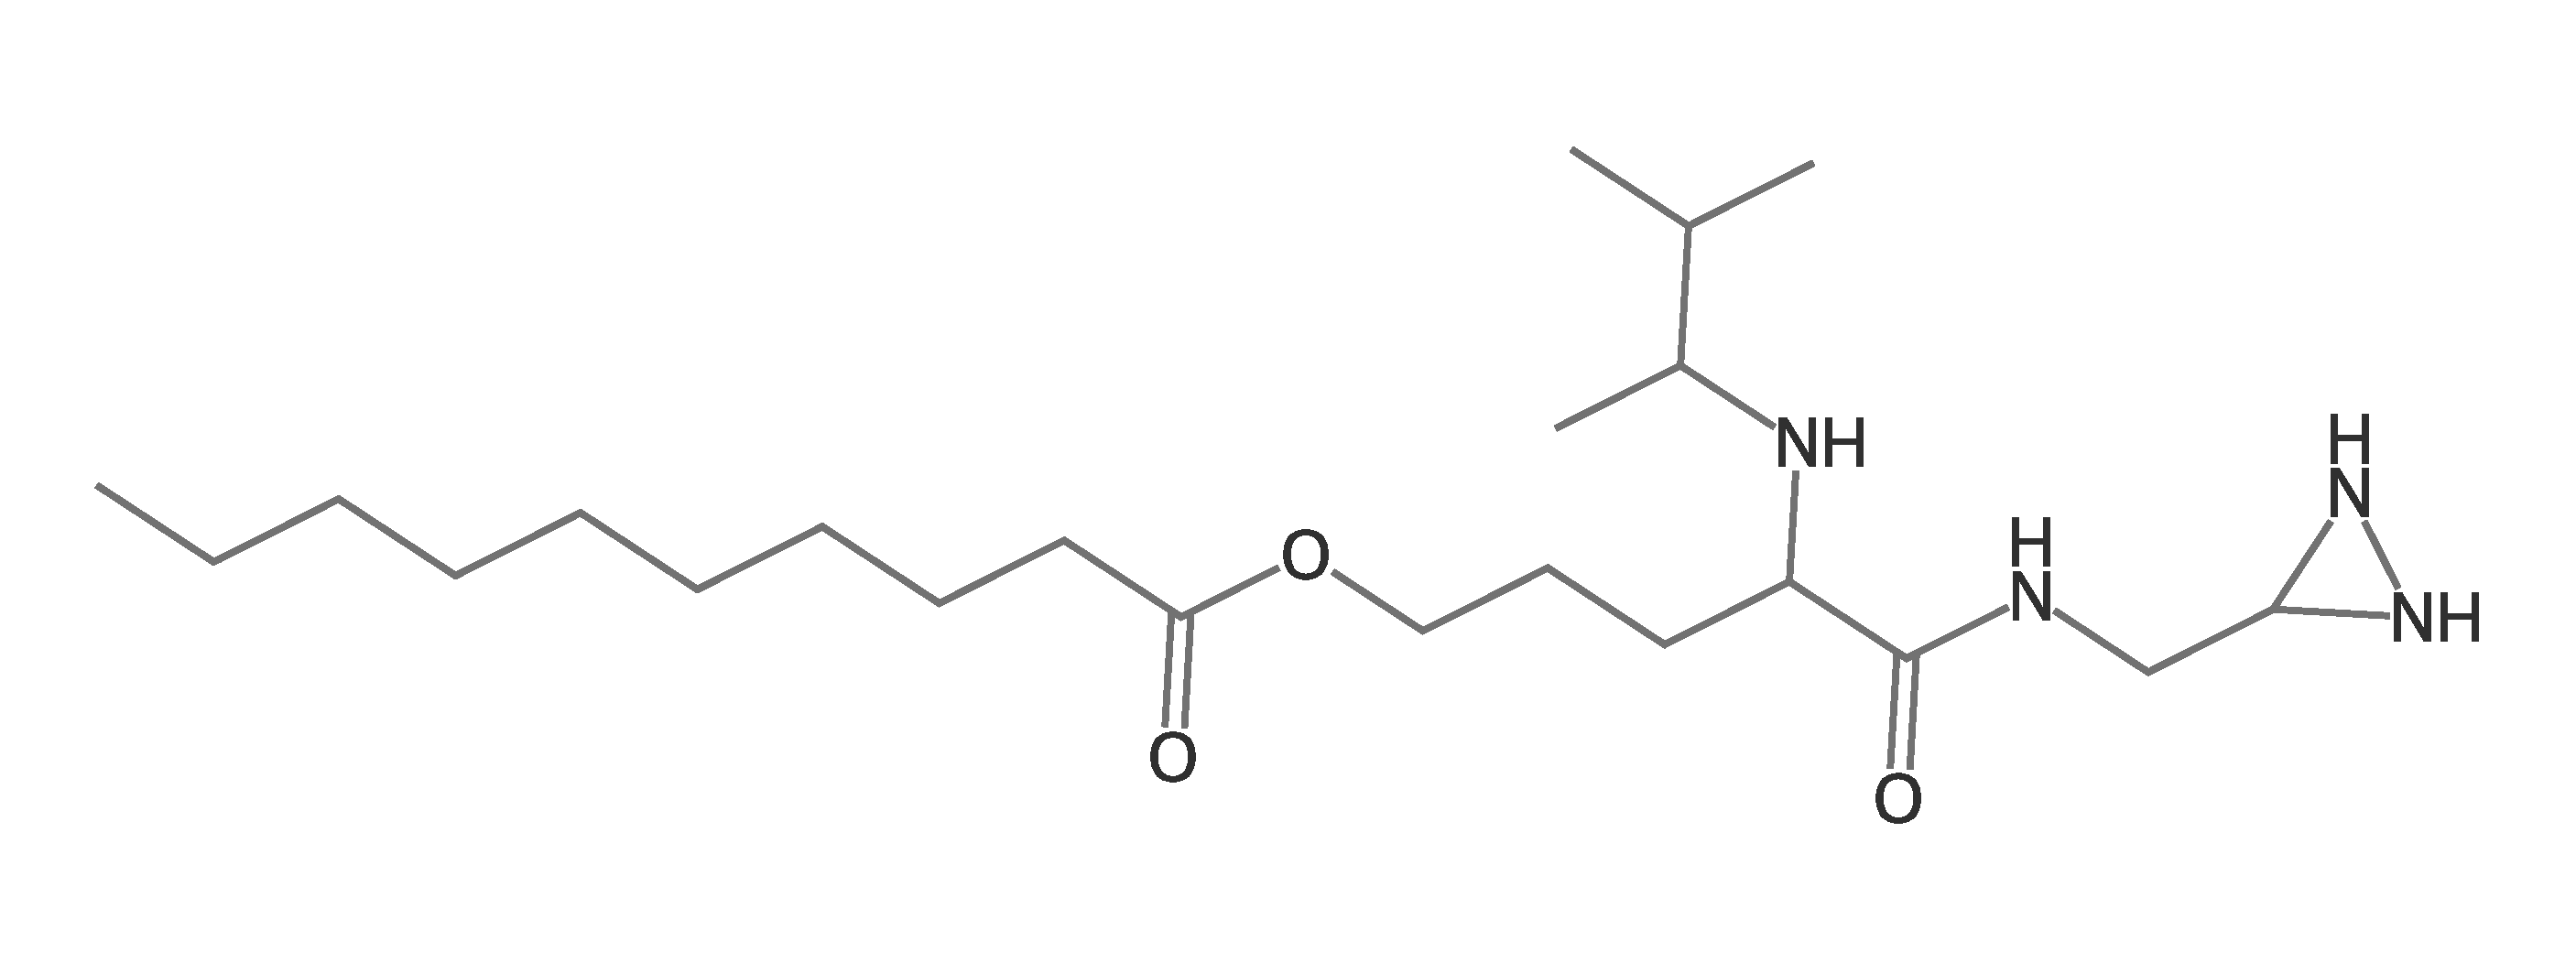
\includegraphics[width=\linewidth,height=\atlasgraphheight,keepaspectratio]{figures/chemical_drawings/atlas_07_2d.pdf}
\par\vspace{\atlassmilesskip}
{\atlassmilesstyle CCCCCCCCCC(=O)OCCCC(NC(C)C(C\allowbreak{})C)C(=O)NCC1NN1\par}
\end{minipage}
&
\begin{minipage}[c][\atlasrowheight][c]{\atlasprecursorwidth}
\centering
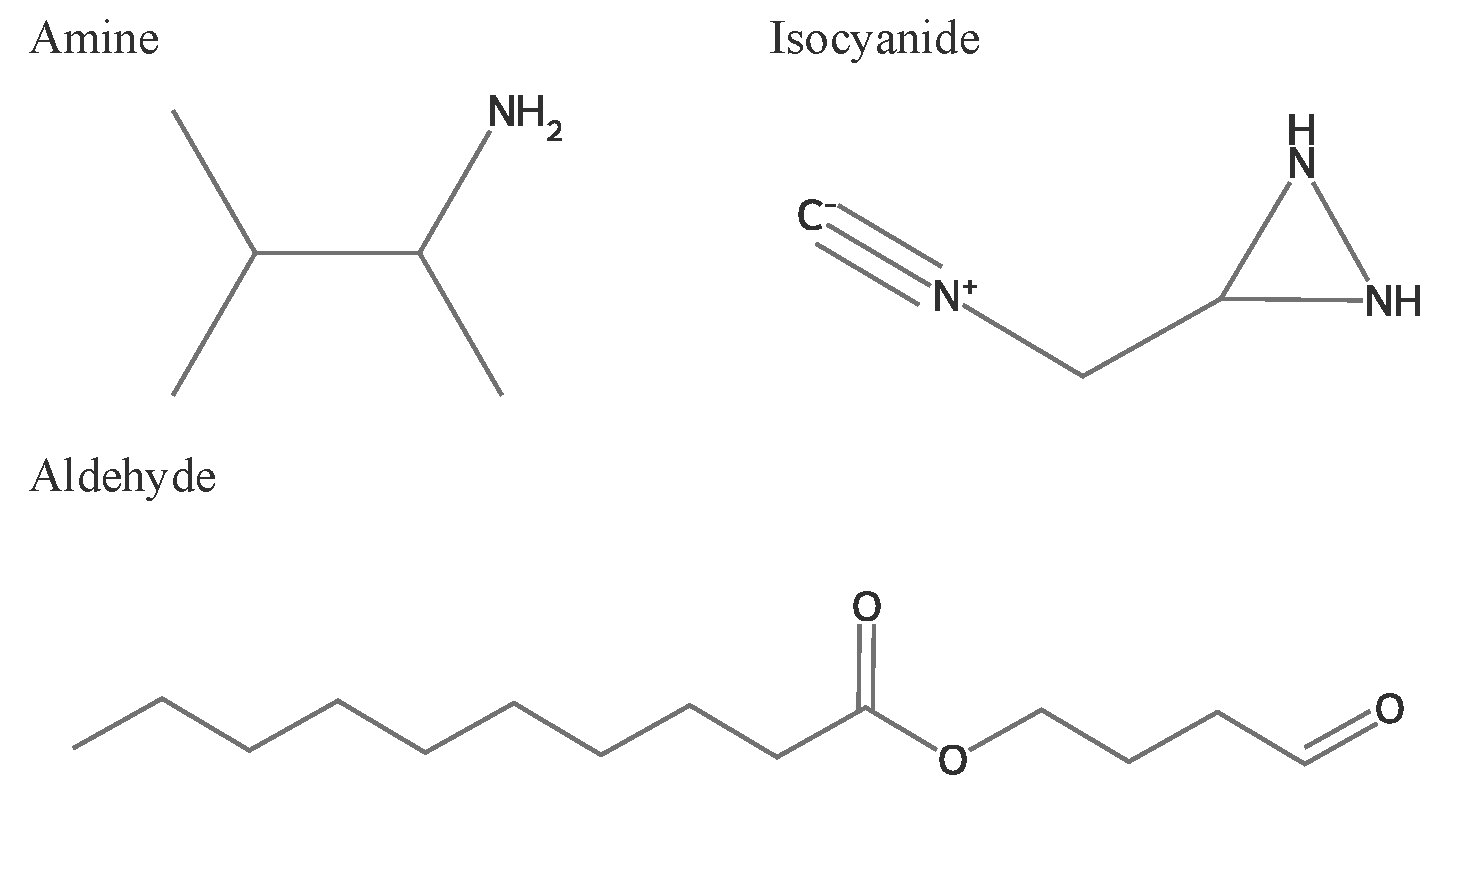
\includegraphics[width=\linewidth,height=\atlasprecursorheight,keepaspectratio]{figures/chemical_drawings/atlas_07_precursors.pdf}
\end{minipage}\\
\atlasrank{8}
&
\begin{minipage}[c][\atlasrowheight][c]{\atlasgraphwidth}
\centering
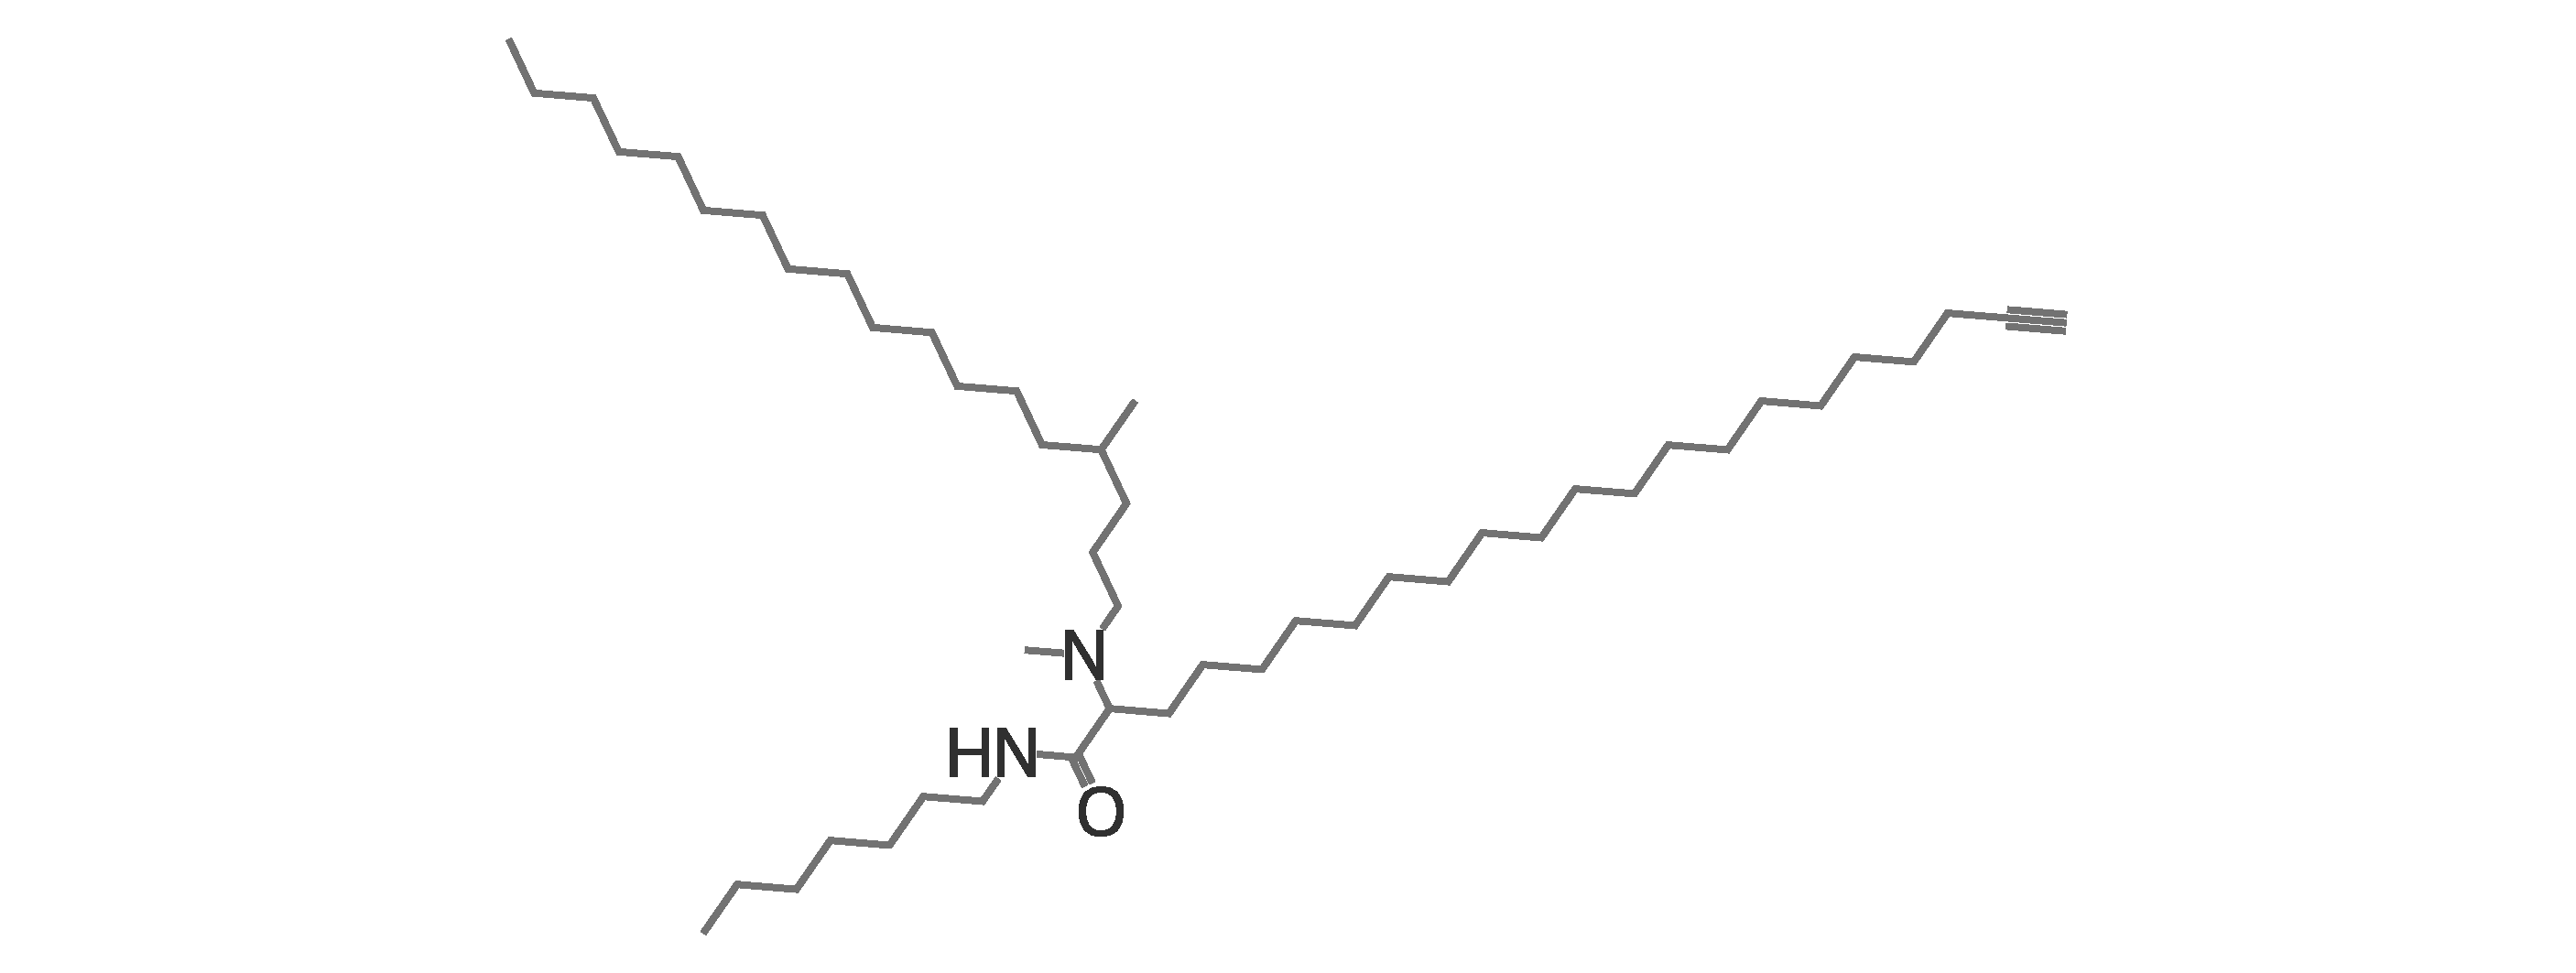
\includegraphics[width=\linewidth,height=\atlasgraphheight,keepaspectratio]{figures/chemical_drawings/atlas_08_2d.pdf}
\par\vspace{\atlassmilesskip}
{\atlassmilesstyle C\#CCCCCCCCCCCCCCCCCCCC(C(=O)\allowbreak{}NCCCCCCC)N(C)CCCC(C)CCCCCCCC\allowbreak{}CCCCCC\par}
\end{minipage}
&
\begin{minipage}[c][\atlasrowheight][c]{\atlasprecursorwidth}
\centering
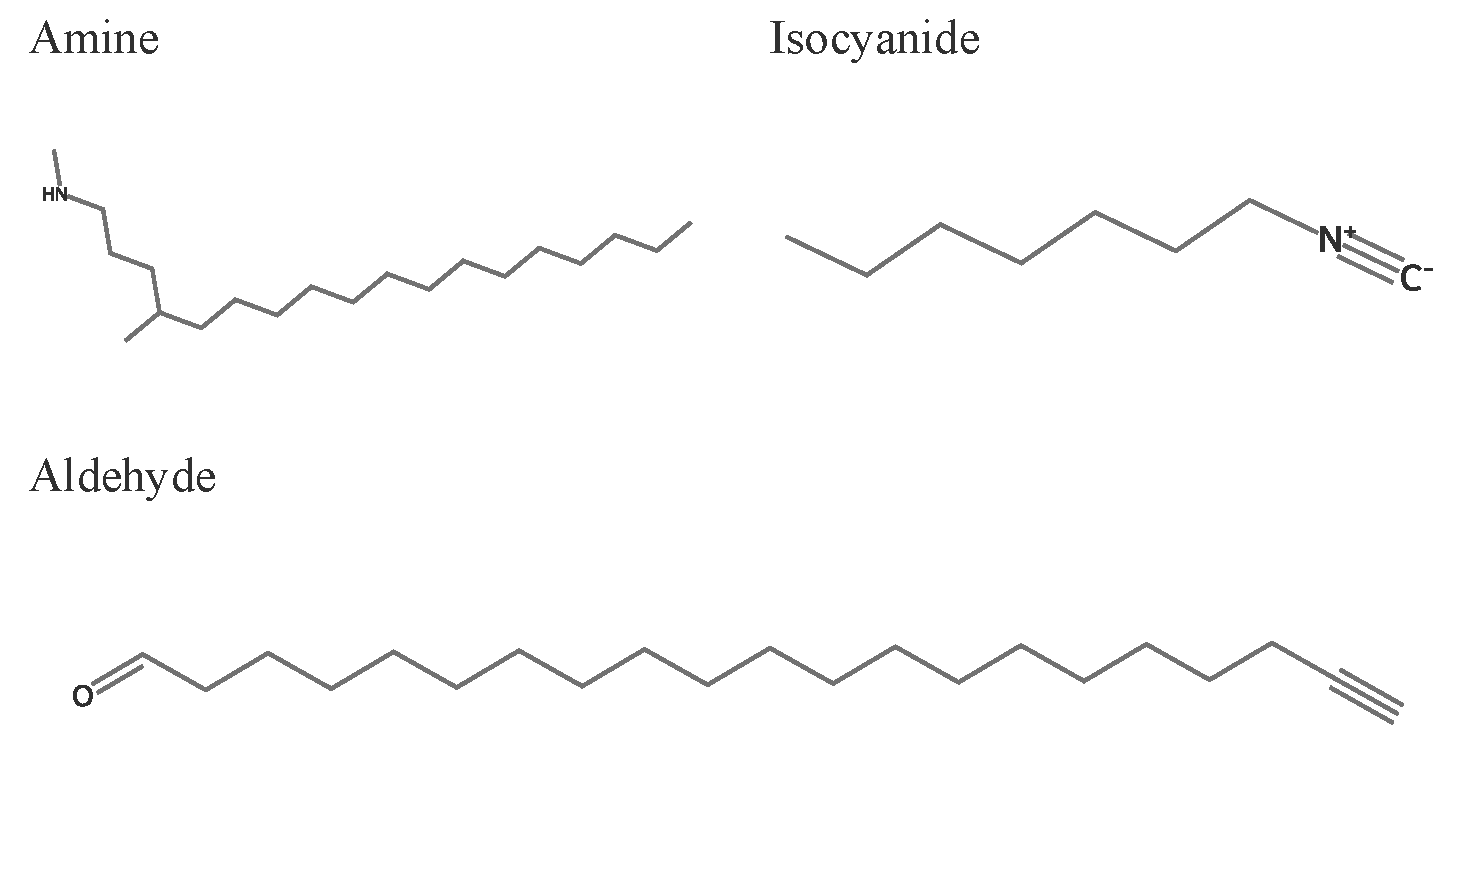
\includegraphics[width=\linewidth,height=\atlasprecursorheight,keepaspectratio]{figures/chemical_drawings/atlas_08_precursors.pdf}
\end{minipage}\\
\atlasrank{9}
&
\begin{minipage}[c][\atlasrowheight][c]{\atlasgraphwidth}
\centering
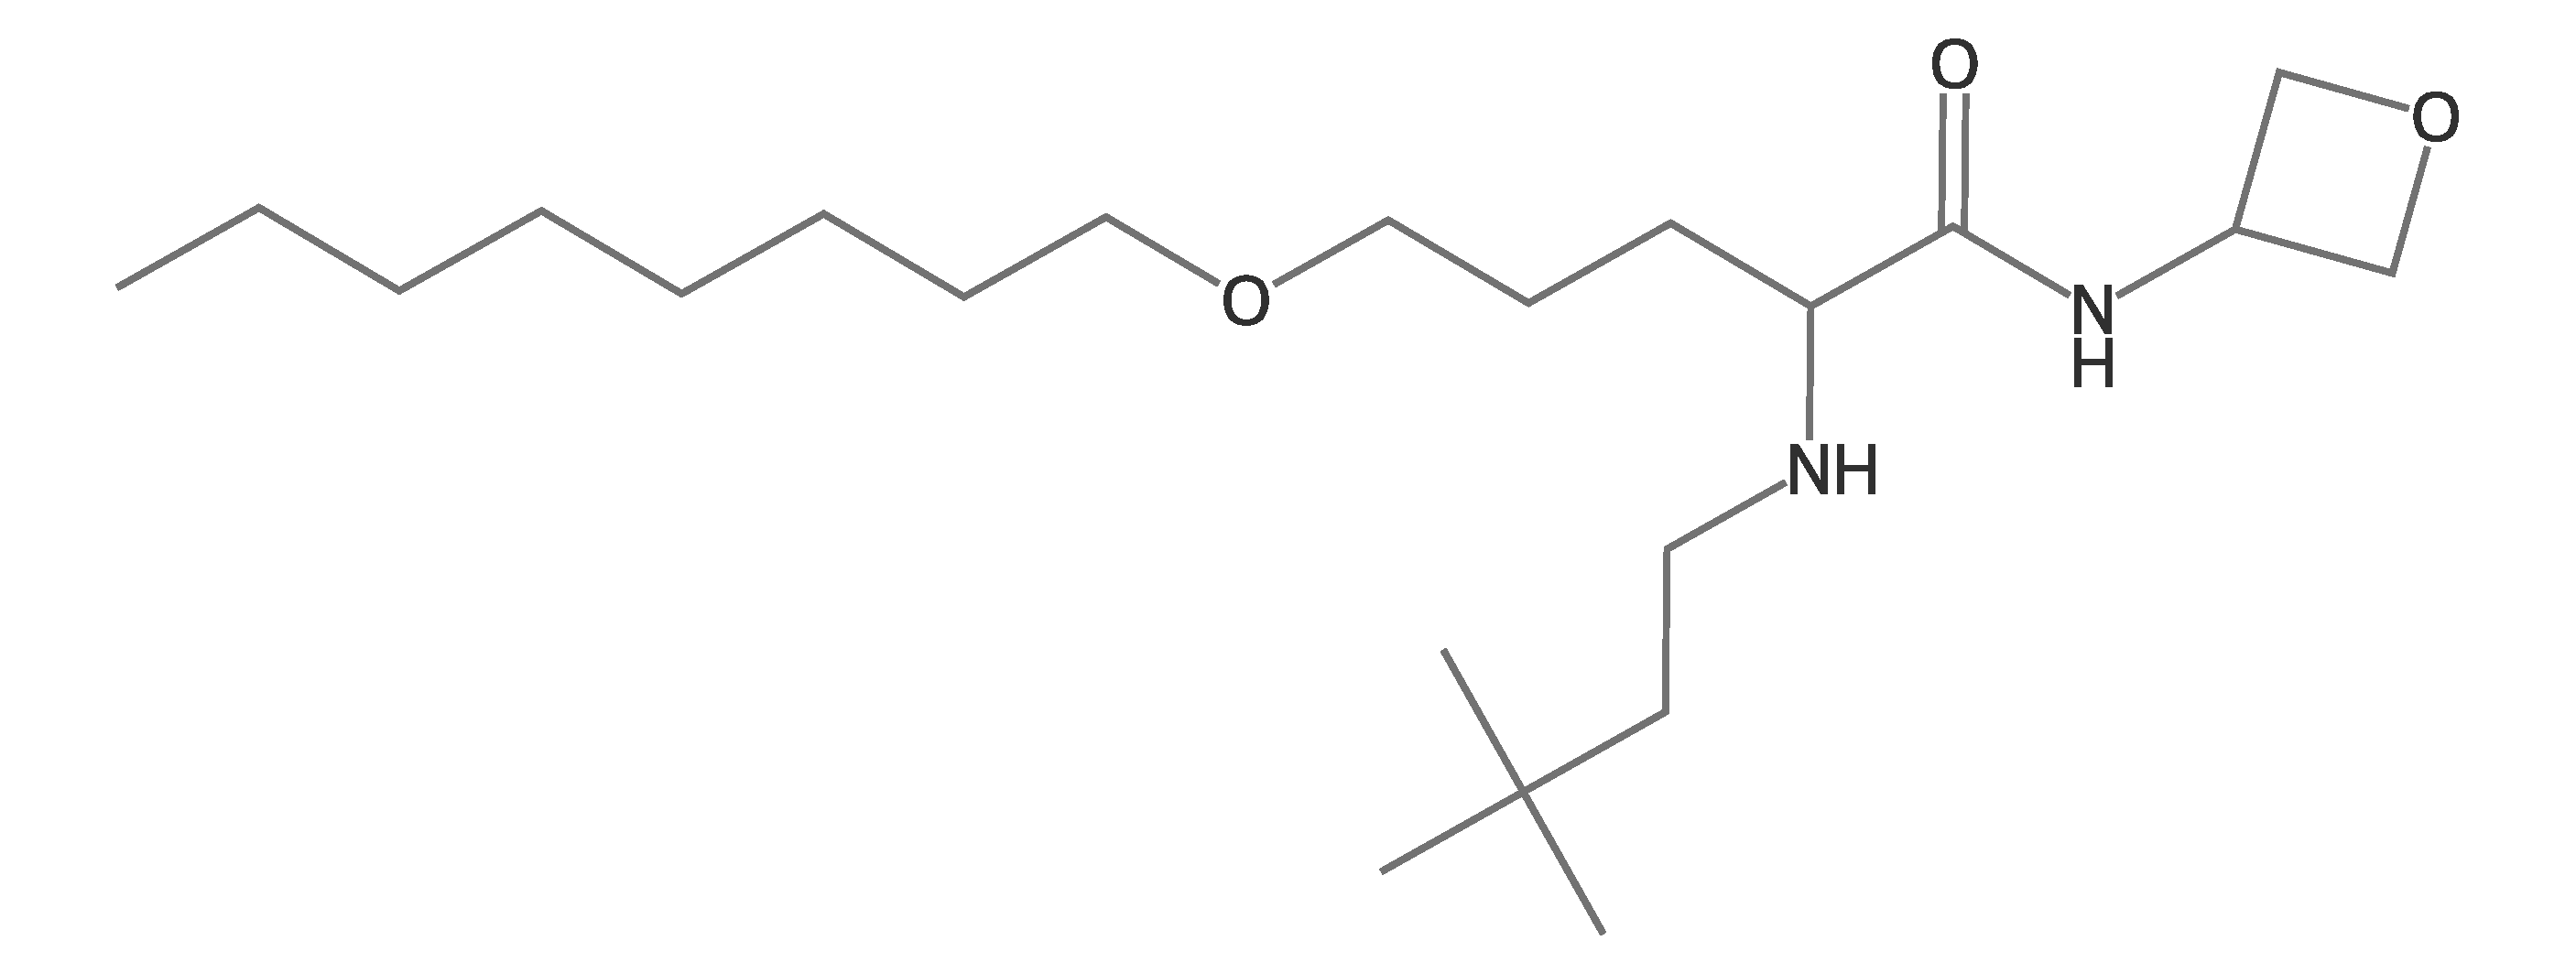
\includegraphics[width=\linewidth,height=\atlasgraphheight,keepaspectratio]{figures/chemical_drawings/atlas_09_2d.pdf}
\par\vspace{\atlassmilesskip}
{\atlassmilesstyle CCCCCCCCOCCCC(NCCC(C)(C)C)C(\allowbreak{}=O)NC1COC1\par}
\end{minipage}
&
\begin{minipage}[c][\atlasrowheight][c]{\atlasprecursorwidth}
\centering
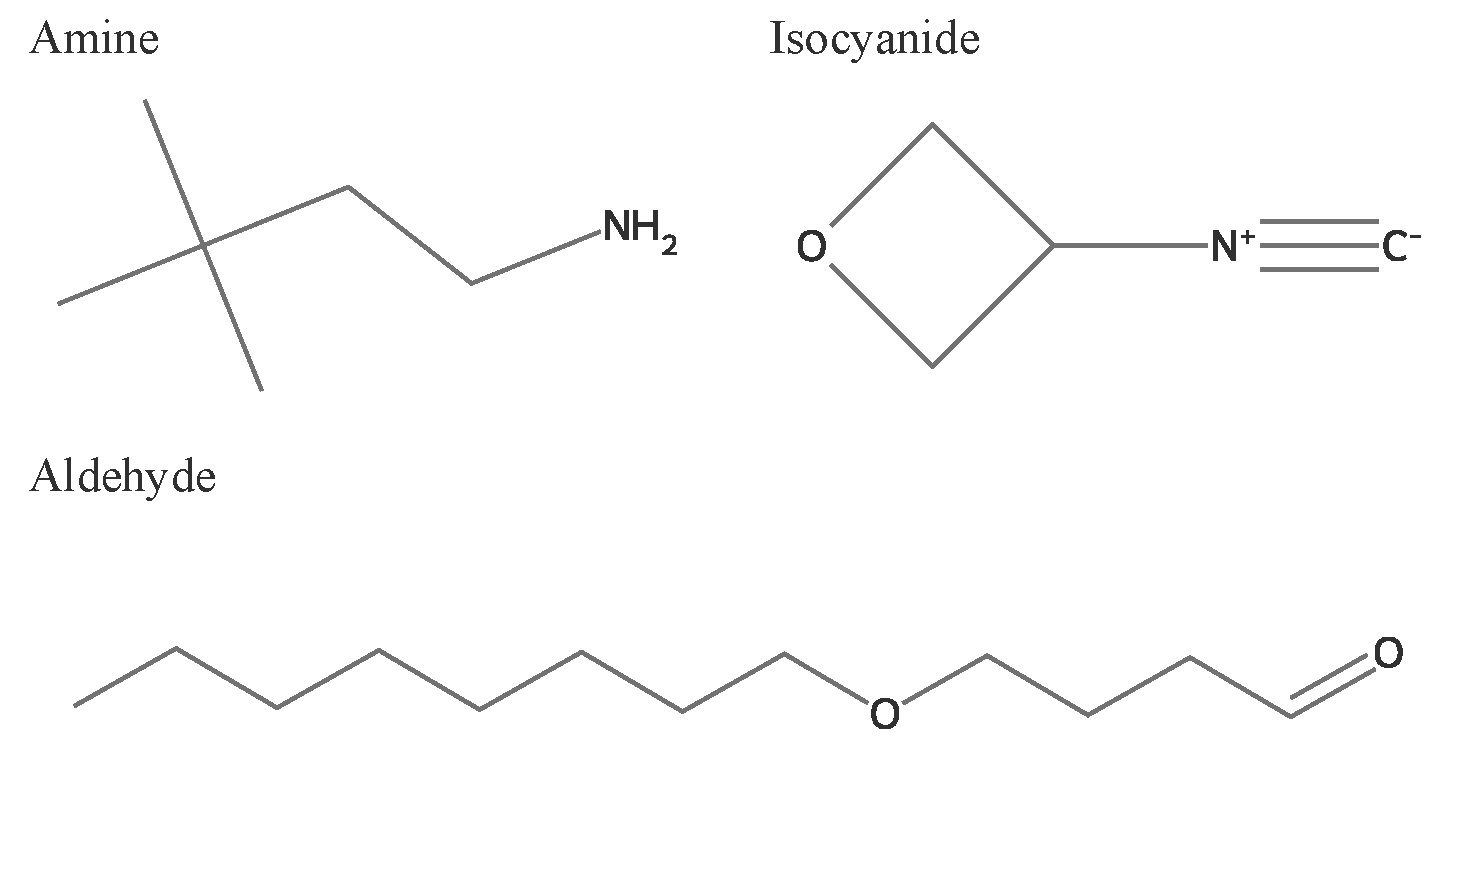
\includegraphics[width=\linewidth,height=\atlasprecursorheight,keepaspectratio]{figures/chemical_drawings/atlas_09_precursors.pdf}
\end{minipage}\\
\atlasrank{10}
&
\begin{minipage}[c][\atlasrowheight][c]{\atlasgraphwidth}
\centering
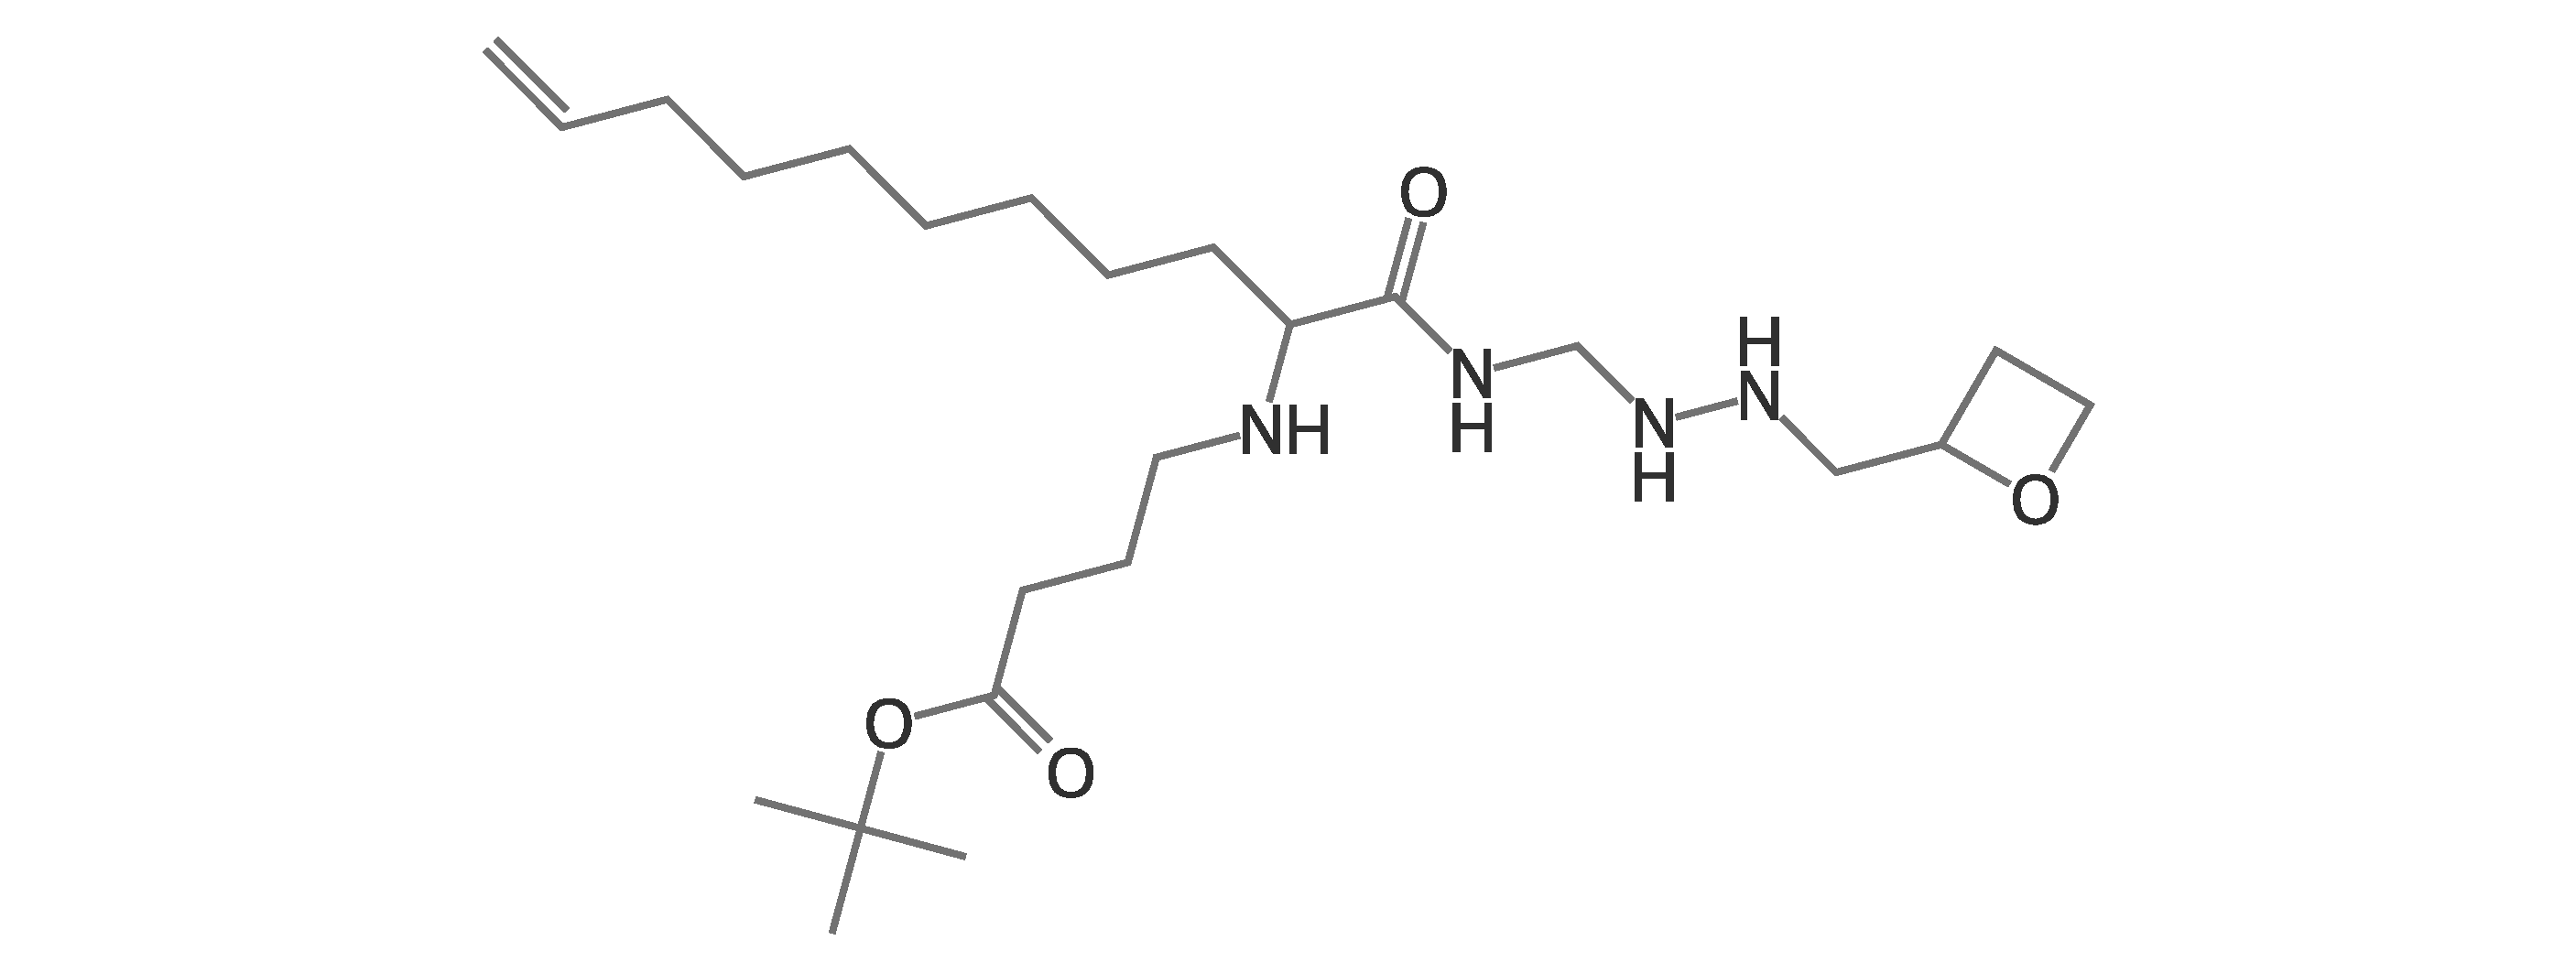
\includegraphics[width=\linewidth,height=\atlasgraphheight,keepaspectratio]{figures/chemical_drawings/atlas_10_2d.pdf}
\par\vspace{\atlassmilesskip}
{\atlassmilesstyle C=CCCCCCCCC(NCCCC(=O)OC(C)(C\allowbreak{})C)C(=O)NCNNCC1CCO1\par}
\end{minipage}
&
\begin{minipage}[c][\atlasrowheight][c]{\atlasprecursorwidth}
\centering
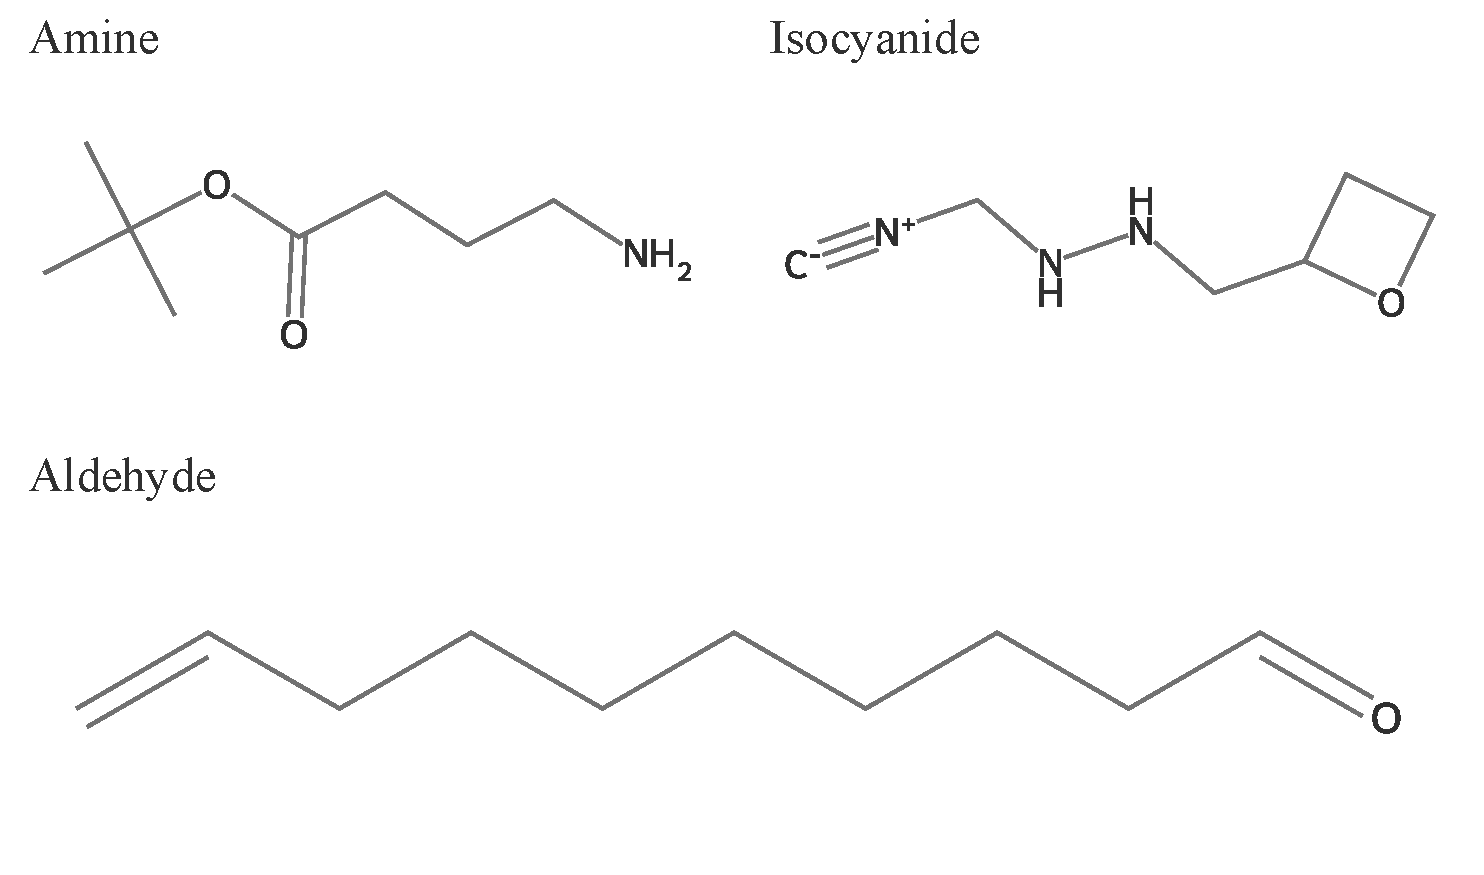
\includegraphics[width=\linewidth,height=\atlasprecursorheight,keepaspectratio]{figures/chemical_drawings/atlas_10_precursors.pdf}
\end{minipage}\\
\atlasrank{11}
&
\begin{minipage}[c][\atlasrowheight][c]{\atlasgraphwidth}
\centering
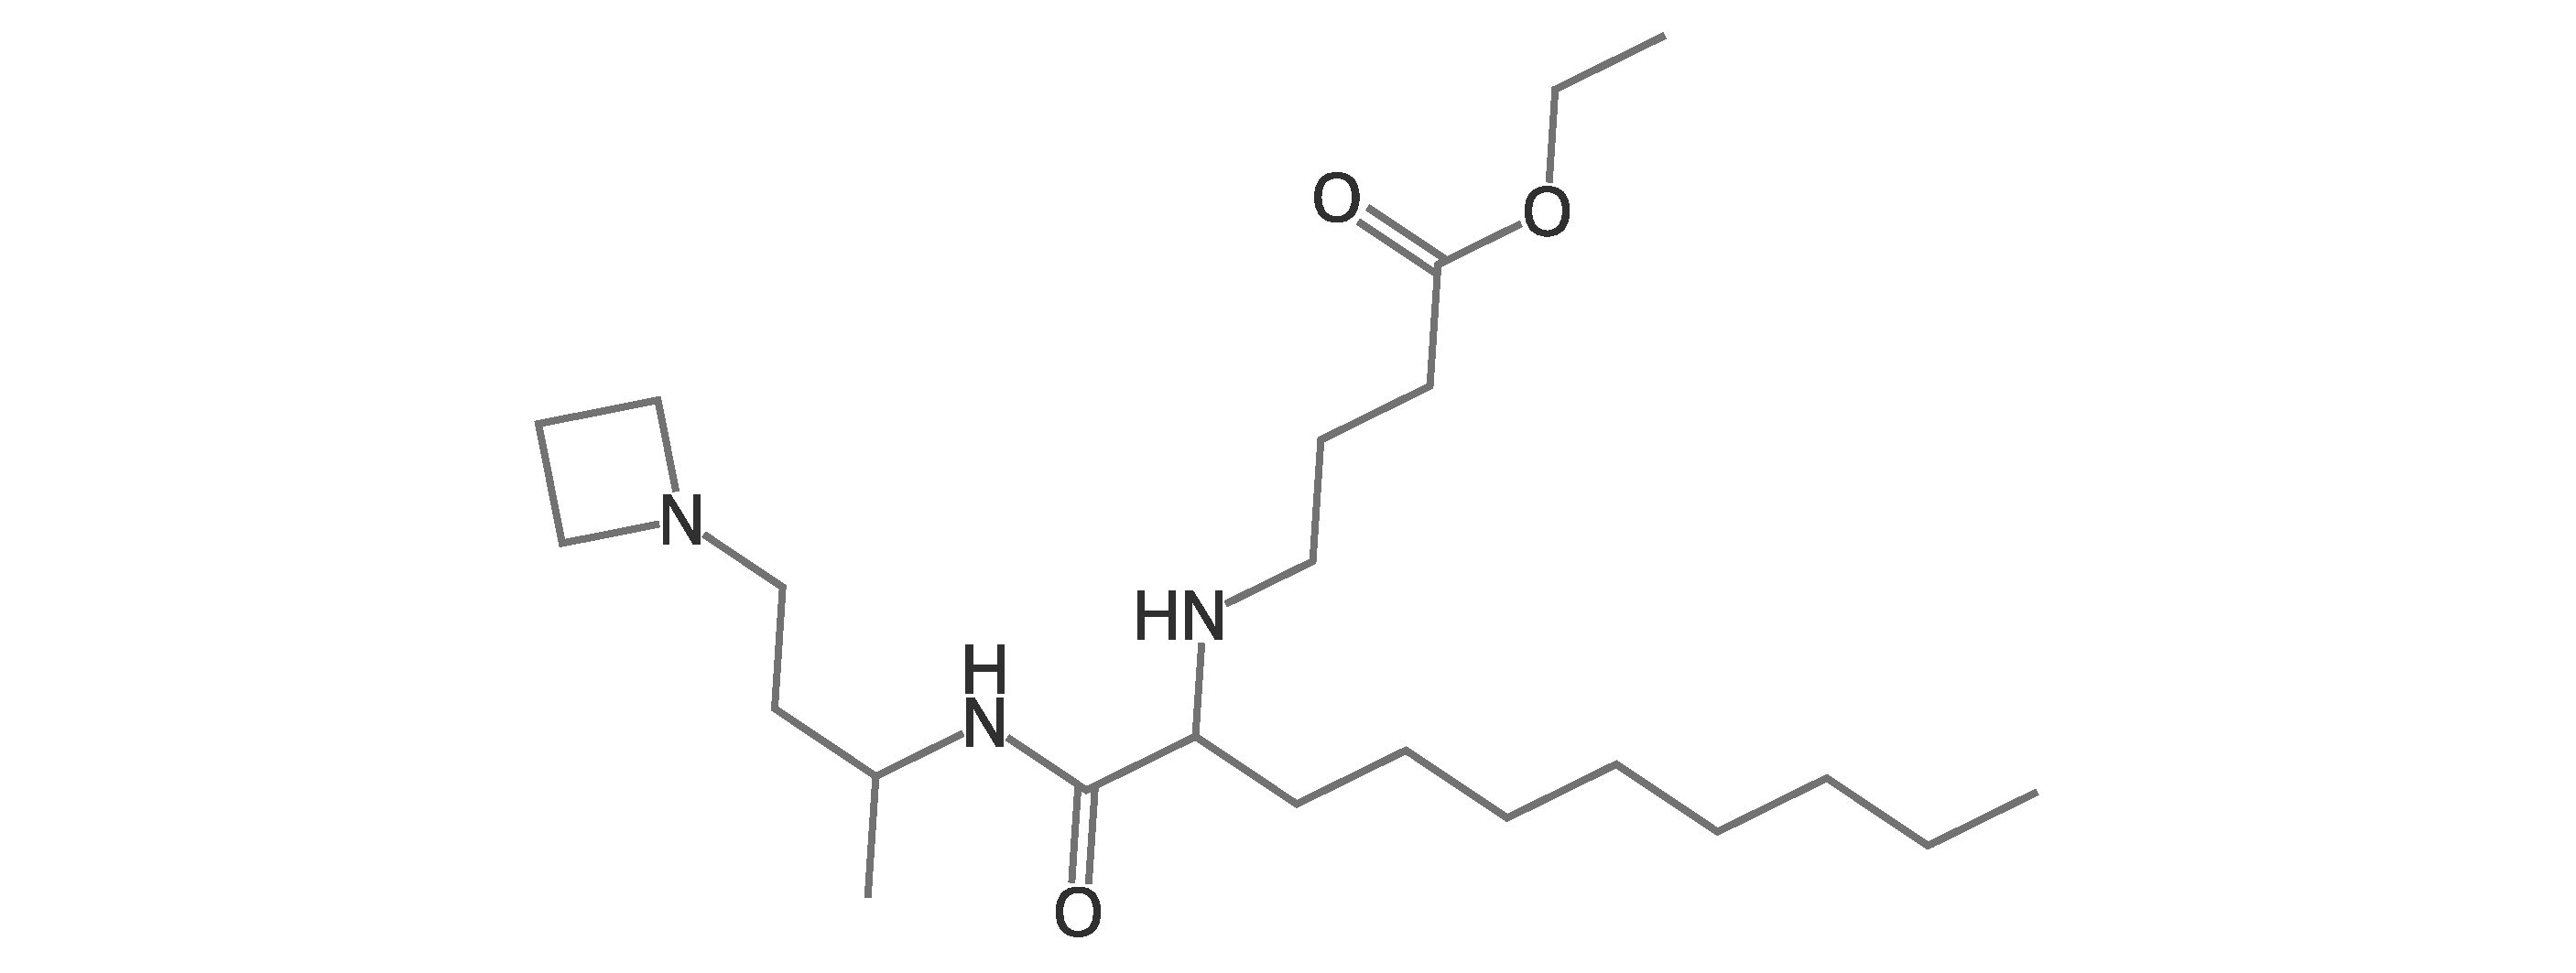
\includegraphics[width=\linewidth,height=\atlasgraphheight,keepaspectratio]{figures/chemical_drawings/atlas_11_2d.pdf}
\par\vspace{\atlassmilesskip}
{\atlassmilesstyle CCCCCCCCC(NCCCC(=O)OCC)C(=O)\allowbreak{}NC(C)CCN1CCC1\par}
\end{minipage}
&
\begin{minipage}[c][\atlasrowheight][c]{\atlasprecursorwidth}
\centering
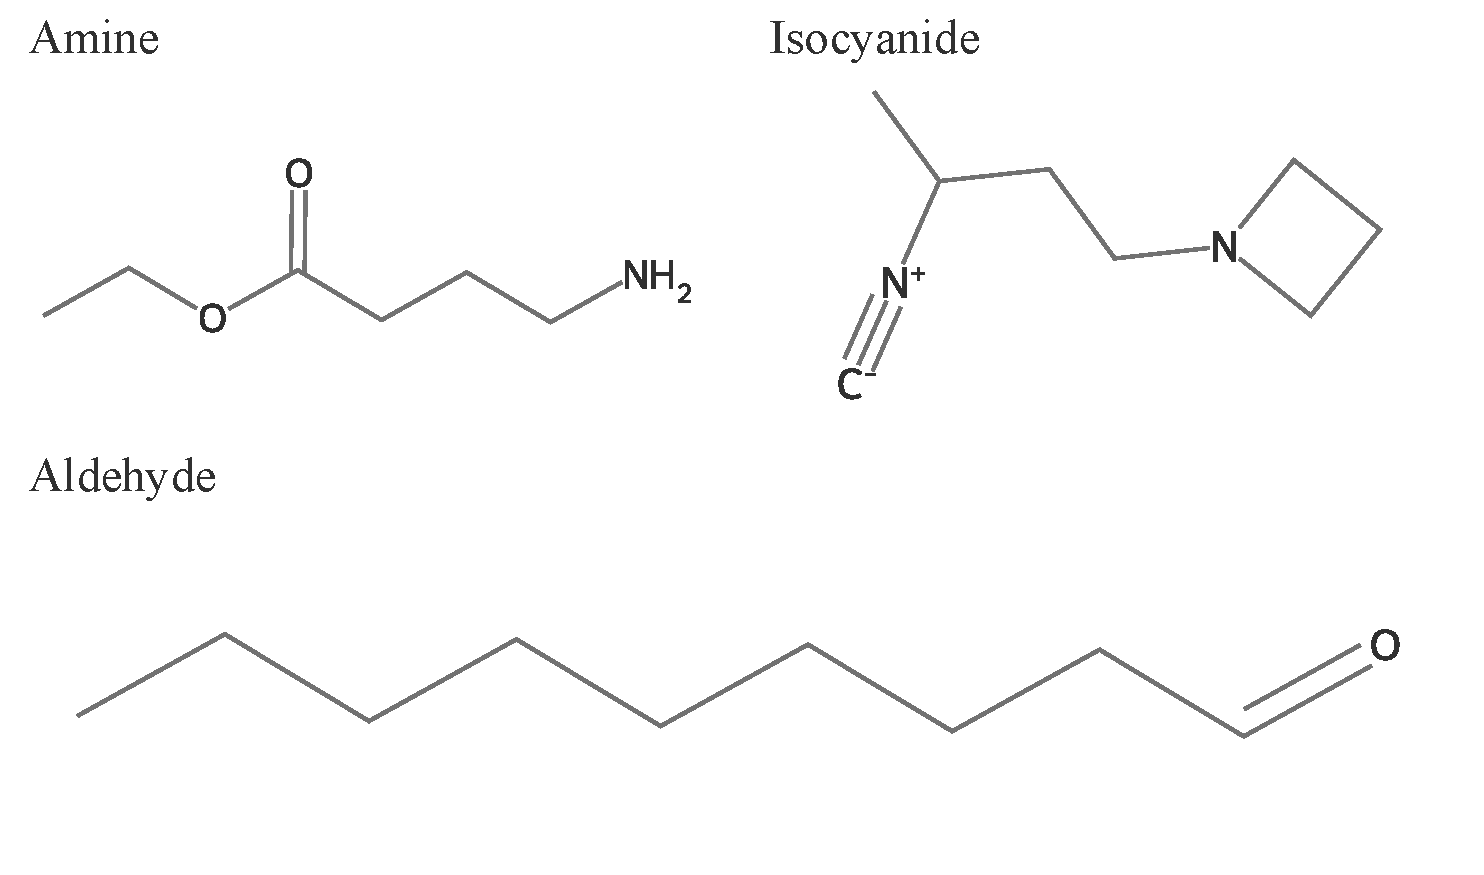
\includegraphics[width=\linewidth,height=\atlasprecursorheight,keepaspectratio]{figures/chemical_drawings/atlas_11_precursors.pdf}
\end{minipage}\\
\atlasrank{12}
&
\begin{minipage}[c][\atlasrowheight][c]{\atlasgraphwidth}
\centering
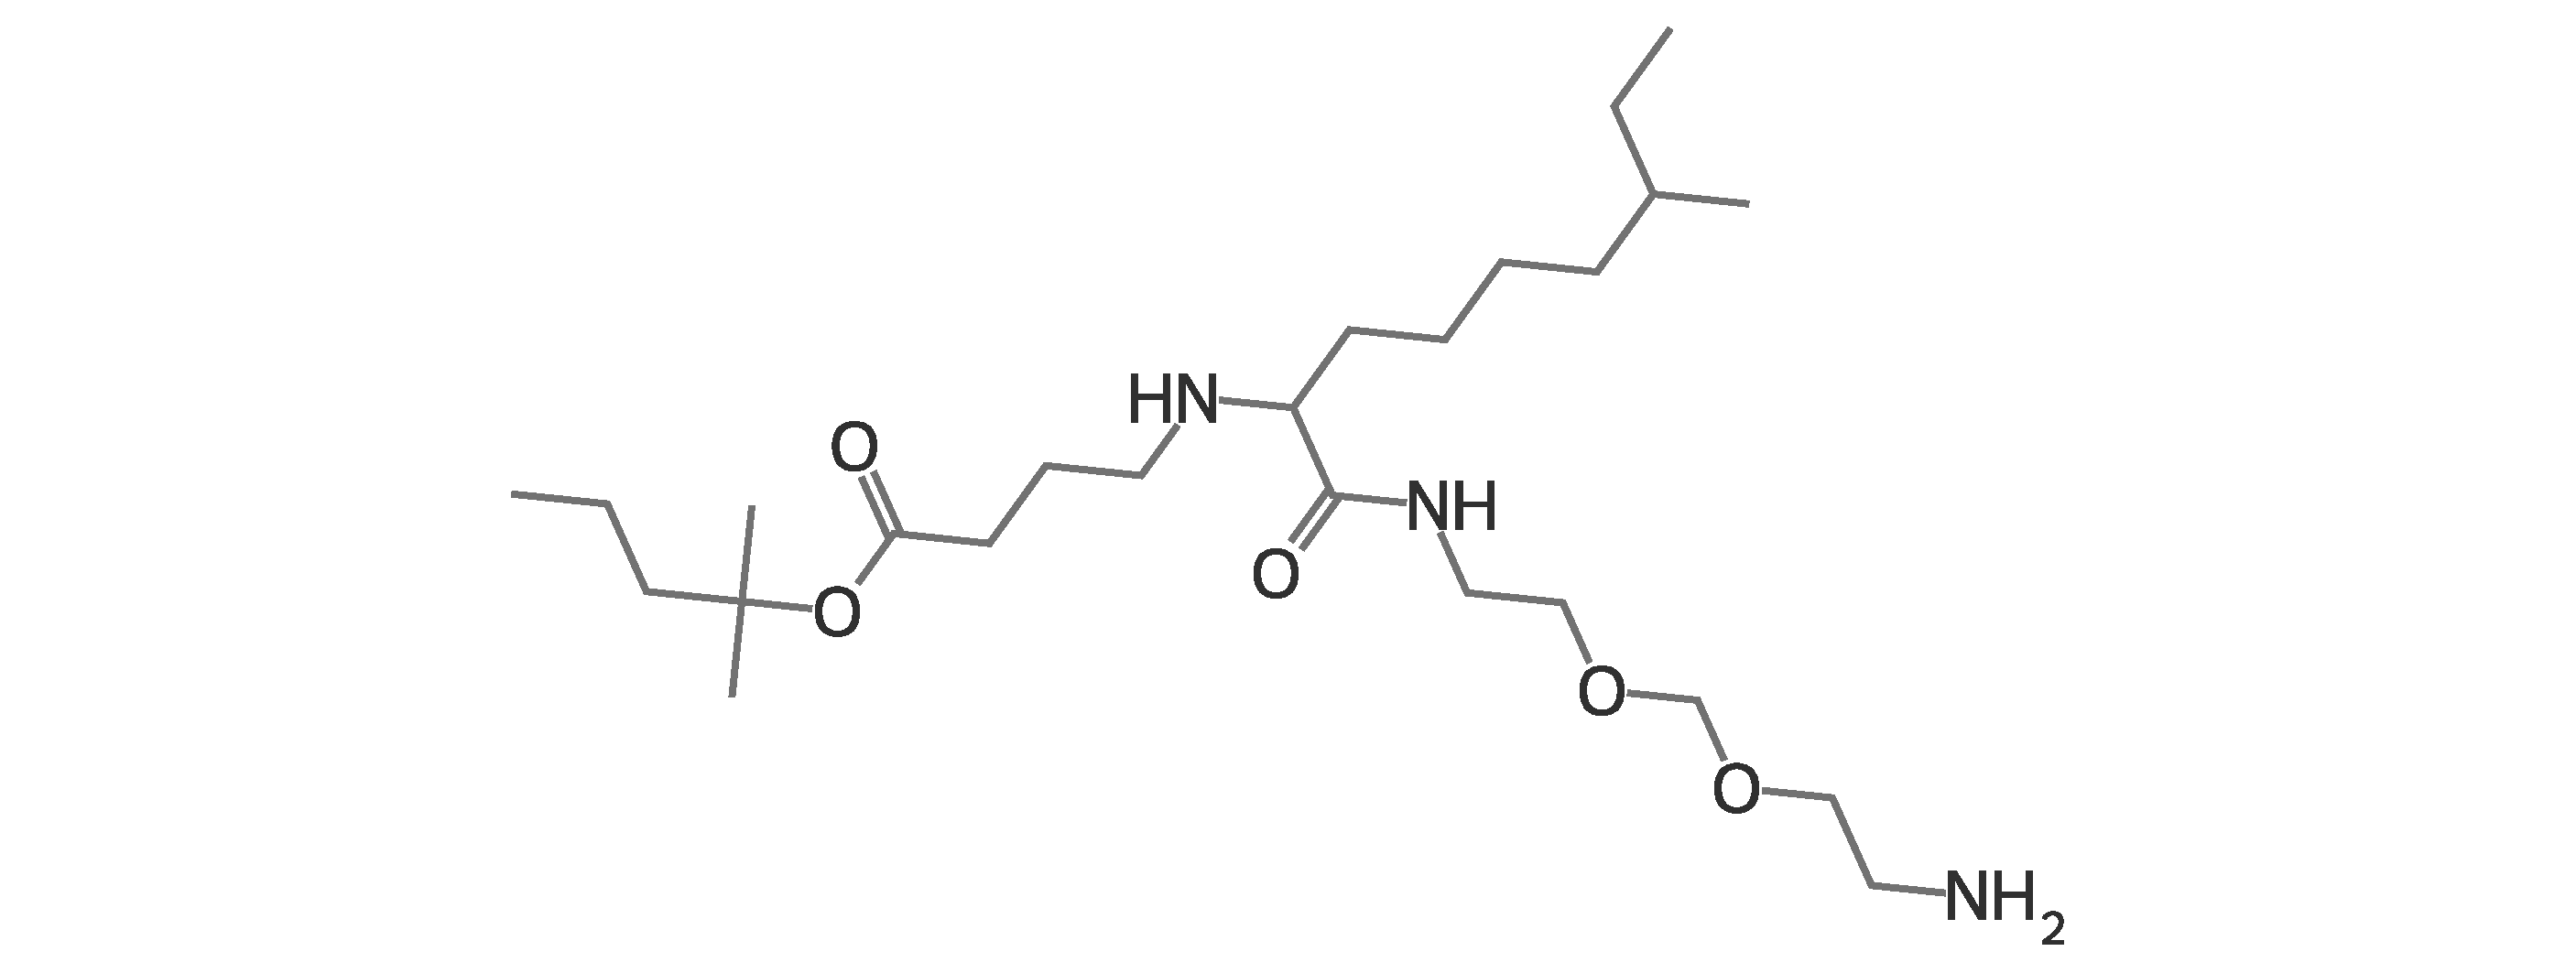
\includegraphics[width=\linewidth,height=\atlasgraphheight,keepaspectratio]{figures/chemical_drawings/atlas_12_2d.pdf}
\par\vspace{\atlassmilesskip}
{\atlassmilesstyle CCCC(C)(C)OC(=O)CCCNC(CCCCC(\allowbreak{}C)CC)C(=O)NCCOCOCCN\par}
\end{minipage}
&
\begin{minipage}[c][\atlasrowheight][c]{\atlasprecursorwidth}
\centering
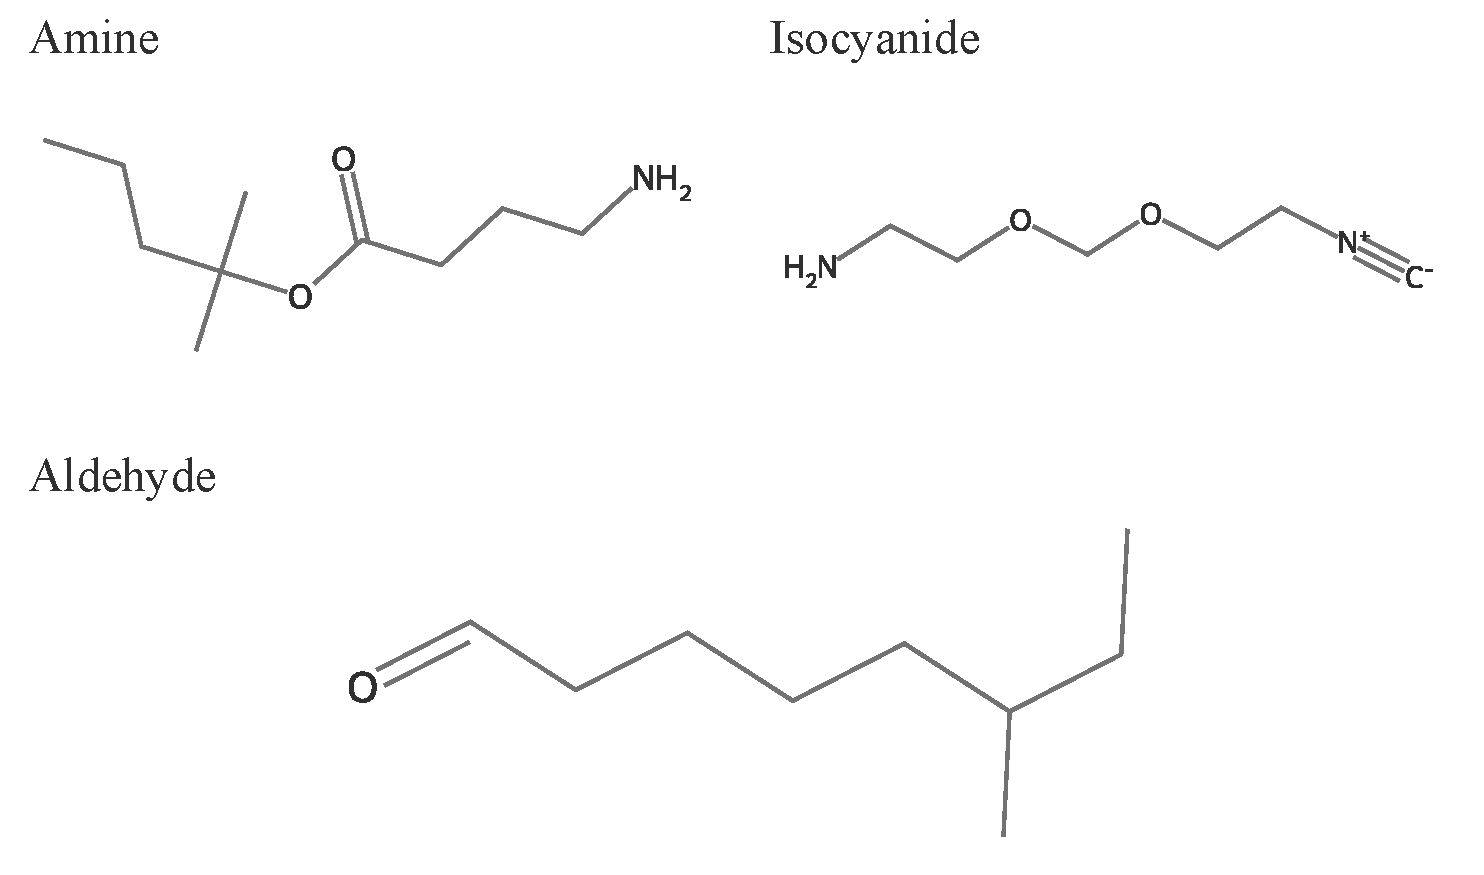
\includegraphics[width=\linewidth,height=\atlasprecursorheight,keepaspectratio]{figures/chemical_drawings/atlas_12_precursors.pdf}
\end{minipage}\\
%
\end{longtable}
\endgroup

\end{document}
